%&preformat-disser
\RequirePackage[l2tabu,orthodox]{nag} % Раскомментировав, можно в логе получать рекомендации относительно правильного использования пакетов и предупреждения об устаревших и нерекомендуемых пакетах
% Формат А4, 14pt (ГОСТ Р 7.0.11-2011, 5.3.6)
\documentclass[a4paper,14pt,oneside,openany]{memoir}

%%%%%%%%%%%%%%%%%%%%%%%%%%%%%%%%%%%%%%%%%%%%%%%%%%%%%%
%%%% Файл упрощённых настроек шаблона диссертации %%%%
%%%%%%%%%%%%%%%%%%%%%%%%%%%%%%%%%%%%%%%%%%%%%%%%%%%%%%

%%% Инициализирование переменных, не трогать!  %%%
\newcounter{intvl}
\newcounter{otstup}
\newcounter{contnumeq}
\newcounter{contnumfig}
\newcounter{contnumtab}
\newcounter{pgnum}
\newcounter{chapstyle}
\newcounter{headingdelim}
\newcounter{headingalign}
\newcounter{headingsize}
\newcounter{tabcap}
\newcounter{tablaba}
\newcounter{tabtita}
\newcounter{usefootcite}
%%%%%%%%%%%%%%%%%%%%%%%%%%%%%%%%%%%%%%%%%%%%%%%%%%

%%% Область упрощённого управления оформлением %%%

%% Интервал между заголовками и между заголовком и текстом
% Заголовки отделяют от текста сверху и снизу тремя интервалами (ГОСТ Р 7.0.11-2011, 5.3.5)
\setcounter{intvl}{3}               % Коэффициент кратности к размеру шрифта

%% Отступы у заголовков в тексте
\setcounter{otstup}{0}              % 0 --- без отступа; 1 --- абзацный отступ

%% Нумерация формул, таблиц и рисунков
\setcounter{contnumeq}{0}           % Нумерация формул: 0 --- пораздельно (во введении подряд, без номера раздела); 1 --- сквозная нумерация по всей диссертации
\setcounter{contnumfig}{0}          % Нумерация рисунков: 0 --- пораздельно (во введении подряд, без номера раздела); 1 --- сквозная нумерация по всей диссертации
\setcounter{contnumtab}{1}          % Нумерация таблиц: 0 --- пораздельно (во введении подряд, без номера раздела); 1 --- сквозная нумерация по всей диссертации

%% Оглавление
\setcounter{pgnum}{1}               % 0 --- номера страниц никак не обозначены; 1 --- Стр. над номерами страниц (дважды компилировать после изменения)
\settocdepth{subsection}            % до какого уровня подразделов выносить в оглавление
\setsecnumdepth{subsection}         % до какого уровня нумеровать подразделы


%% Текст и форматирование заголовков
\setcounter{chapstyle}{1}           % 0 --- разделы только под номером; 1 --- разделы с названием "Глава" перед номером
\setcounter{headingdelim}{1}        % 0 --- номер отделен пропуском в 1em или \quad; 1 --- номера разделов и приложений отделены точкой с пробелом, подразделы пропуском без точки; 2 --- номера разделов, подразделов и приложений отделены точкой с пробелом.

%% Выравнивание заголовков в тексте
\setcounter{headingalign}{0}        % 0 --- по центру; 1 --- по левому краю

%% Размеры заголовков в тексте
\setcounter{headingsize}{0}         % 0 --- по ГОСТ, все всегда 14 пт; 1 --- пропорционально изменяющийся размер в зависимости от базового шрифта

%% Подпись таблиц
\setcounter{tabcap}{0}              % 0 --- по ГОСТ, номер таблицы и название разделены тире, выровнены по левому краю, при необходимости на нескольких строках; 1 --- подпись таблицы не по ГОСТ, на двух и более строках, дальнейшие настройки: 
%Выравнивание первой строки, с подписью и номером
\setcounter{tablaba}{2}             % 0 --- по левому краю; 1 --- по центру; 2 --- по правому краю
%Выравнивание строк с самим названием таблицы
\setcounter{tabtita}{1}             % 0 --- по левому краю; 1 --- по центру; 2 --- по правому краю
%Разделитель записи «Таблица #» и названия таблицы
\newcommand{\tablabelsep}{ }

%% Подпись рисунков
%Разделитель записи «Рисунок #» и названия рисунка
\newcommand{\figlabelsep}{~\cyrdash\ } % (ГОСТ 2.105, 4.3.1) % "--- здесь не работает

%%% Цвета гиперссылок %%%
% Latex color definitions: http://latexcolor.com/
\definecolor{linkcolor}{rgb}{0.9,0,0}
\definecolor{citecolor}{rgb}{0,0.6,0}
\definecolor{urlcolor}{rgb}{0,0,1}
%\definecolor{linkcolor}{rgb}{0,0,0} %black
%\definecolor{citecolor}{rgb}{0,0,0} %black
%\definecolor{urlcolor}{rgb}{0,0,0} %black
            % общие настройки шаблона
%%% Проверка используемого TeX-движка %%%
\RequirePackage{ifxetex, ifluatex}
\newif\ifxetexorluatex   % определяем новый условный оператор (http://tex.stackexchange.com/a/47579)
\ifxetex
    \xetexorluatextrue
\else
    \ifluatex
        \xetexorluatextrue
    \else
        \xetexorluatexfalse
    \fi
\fi

\newif\ifsynopsis           % Условие, проверяющее, что документ --- автореферат

\RequirePackage{etoolbox}[2015/08/02]               % Для продвинутой проверки разных условий

%%% Поля и разметка страницы %%%
\usepackage{pdflscape}                              % Для включения альбомных страниц
\usepackage{geometry}                               % Для последующего задания полей

%%% Математические пакеты %%%
\usepackage{amsthm,amsmath,amscd}   % Математические дополнения от AMS
\usepackage{amsfonts,amssymb}       % Математические дополнения от AMS
\usepackage{mathtools}              % Добавляет окружение multlined

%%%% Установки для размера шрифта 14 pt %%%%
%% Формирование переменных и констант для сравнения (один раз для всех подключаемых файлов)%%
%% должно располагаться до вызова пакета fontspec или polyglossia, потому что они сбивают его работу
\newlength{\curtextsize}
\newlength{\bigtextsize}
\setlength{\bigtextsize}{13.9pt}

\makeatletter
%\show\f@size                                       % неплохо для отслеживания, но вызывает стопорение процесса, если документ компилируется без команды  -interaction=nonstopmode 
\setlength{\curtextsize}{\f@size pt}
\makeatother

%%% Кодировки и шрифты %%%
\ifxetexorluatex
    \usepackage{polyglossia}[2014/05/21]            % Поддержка многоязычности (fontspec подгружается автоматически)
\else
   %%% Решение проблемы копирования текста в буфер кракозябрами
    \ifnumequal{\value{usealtfont}}{0}{}{
        \input glyphtounicode.tex
        \input glyphtounicode-cmr.tex %from pdfx package
        \pdfgentounicode=1
    }
    \usepackage{cmap}                               % Улучшенный поиск русских слов в полученном pdf-файле
    \ifnumequal{\value{usealtfont}}{2}{}{
        \defaulthyphenchar=127                      % Если стоит до fontenc, то переносы не впишутся в выделяемый текст при копировании его в буфер обмена
    }
    \usepackage{textcomp}
    \usepackage[T1,T2A]{fontenc}                    % Поддержка русских букв
    \ifnumequal{\value{usealtfont}}{1}{% Используется pscyr, при наличии
        \IfFileExists{pscyr.sty}{\usepackage{pscyr}}{}  % Подключение pscyr
    }{}
    \usepackage[utf8]{inputenc}[2014/04/30]         % Кодировка utf8
    \usepackage[english, main=russian]{babel}[2014/03/24]% Языки: русский, английский
    \ifnumequal{\value{usealtfont}}{2}{
        % http://dxdy.ru/post1238763.html#p1238763
        \usepackage[scaled=0.960]{XCharter}[2017/12/19] % Подключение русифицированных шрифтов XCharter
        \usepackage[charter, vvarbb, scaled=1.048]{newtxmath}[2017/12/14]
        \setDisplayskipStretch{-0.078}
    }{}
\fi

%%% Оформление абзацев %%%
\usepackage{indentfirst}                            % Красная строка

%%% Цвета %%%
\usepackage[dvipsnames, table, hyperref, cmyk]{xcolor} % Совместимо с tikz. Конвертация всех цветов в cmyk заложена как удовлетворение возможного требования типографий. Возможно конвертирование и в rgb.

%%% Таблицы %%%
\usepackage{longtable,ltcaption}                    % Длинные таблицы
\usepackage{multirow,makecell}                      % Улучшенное форматирование таблиц

%%% Общее форматирование
\usepackage{soulutf8}                               % Поддержка переносоустойчивых подчёркиваний и зачёркиваний
\usepackage{icomma}                                 % Запятая в десятичных дробях

%%% Оптимизация расстановки переносов и длины последней строки абзаца
\ifluatex
    \ifnumequal{\value{draft}}{1}{% Черновик
        \usepackage[hyphenation, lastparline, nosingleletter, homeoarchy,
        rivers, draft]{impnattypo}
    }{% Чистовик
        \usepackage[hyphenation, lastparline, nosingleletter]{impnattypo}
    }
\else
    \usepackage[hyphenation, lastparline]{impnattypo}
\fi

%%% Гиперссылки %%%
\usepackage{hyperref}[2012/11/06]

%%% Изображения %%%
\usepackage{graphicx}[2014/04/25]                   % Подключаем пакет работы с графикой

%%% Списки %%%
\usepackage{enumitem}

%%% Счётчики %%%
\usepackage[figure,table]{totalcount}               % Счётчик рисунков и таблиц
\usepackage{totcount}                               % Пакет создания счётчиков на основе последнего номера подсчитываемого элемента (может требовать дважды компилировать документ)
\usepackage{totpages}                               % Счётчик страниц, совместимый с hyperref (ссылается на номер последней страницы). Желательно ставить последним пакетом в преамбуле

%%% Продвинутое управление групповыми ссылками (пока только формулами) %%%
\ifxetexorluatex
    \usepackage{cleveref}                           % cleveref корректно считывает язык из настроек polyglossia
\else
    \usepackage[russian]{cleveref}                  % cleveref имеет сложности со считыванием языка из babel. Такое решение русификации вывода выбрано вместо определения в documentclass из опасности что-то лишнее передать во все остальные пакеты, включая библиографию.
\fi
\creflabelformat{equation}{#2#1#3}                  % Формат по умолчанию ставил круглые скобки вокруг каждого номера ссылки, теперь просто номера ссылок без какого-либо дополнительного оформления
\crefrangelabelformat{equation}{#3#1#4\cyrdash#5#2#6}   % Интервалы в русском языке принято делать через тире, если иное не оговорено


\ifnumequal{\value{draft}}{1}{% Черновик
    \usepackage[firstpage]{draftwatermark}
    \SetWatermarkText{DRAFT}
    \SetWatermarkFontSize{14pt}
    \SetWatermarkScale{15}
    \SetWatermarkAngle{45}
}{}

%%% Цитата, не приводимая в автореферате:
% возможно, актуальна только для biblatex
%\newcommand{\citeinsynopsis}[1]{\ifsynopsis\else ~\cite{#1} \fi}
         % Пакеты общие для диссертации и автореферата
\synopsisfalse                      % Этот документ --- не автореферат
%%% Прикладные пакеты %%% 
%\usepackage{calc}               % Пакет для расчётов параметров, например длины

%%% Для добавления Стр. над номерами страниц в оглавлении
%%% http://tex.stackexchange.com/a/306950
\usepackage{afterpage}

\usepackage{tikz}                   % Продвинутый пакет векторной графики
\usetikzlibrary{chains}             % Для примера tikz рисунка
\usetikzlibrary{shapes.geometric}   % Для примера tikz рисунка
\usetikzlibrary{shapes.symbols}     % Для примера tikz рисунка
\usetikzlibrary{arrows}             % Для примера tikz рисунка
\ifnumequal{\value{imgprecompile}}{1}{% Только если у нас включена предкомпиляция
    \usetikzlibrary{external}   % подключение возможности предкомпиляции
    \tikzexternalize[prefix=Dissertation/images/] % activate! % здесь можно указать отдельную папку для скомпилированных файлов
    \ifxetex
        \tikzset{external/up to date check={diff}}
    \fi
}{}
    % Пакеты для диссертации
\usepackage{tabu, tabulary}  %таблицы с автоматически подбирающейся шириной столбцов
\usepackage{fr-longtable}    %ради \endlasthead

% Листинги с исходным кодом программ
\usepackage{fancyvrb}
\usepackage{listings}
\lccode`\~=0\relax %Без этого хака из-за особенностей пакета listings перестают работать конструкции с \MakeLowercase и т. п. в (xe|lua)latex

% Русская традиция начертания греческих букв
\usepackage{upgreek} % прямые греческие ради русской традиции

%%% Микротипографика
%\ifnumequal{\value{draft}}{0}{% Только если у нас режим чистовика
%    \usepackage[final, babel, shrink=45]{microtype}[2016/05/14] % улучшает представление букв и слов в строках, может помочь при наличии отдельно висящих слов
%}{}

% Отметка о версии черновика на каждой странице
% Чтобы работало надо в своей локальной копии по инструкции
% https://www.ctan.org/pkg/gitinfo2 создать небходимые файлы в папке
% ./git/hooks
% If you’re familiar with tweaking git, you can probably work it out for
% yourself. If not, I suggest you follow these steps:
% 1. First, you need a git repository and working tree. For this example,
% let’s suppose that the root of the working tree is in ~/compsci
% 2. Copy the file post-xxx-sample.txt (which is in the same folder of
% your TEX distribution as this pdf) into the git hooks directory in your
% working copy. In our example case, you should end up with a file called
% ~/compsci/.git/hooks/post-checkout
% 3. If you’re using a unix-like system, don’t forget to make the file executable.
% Just how you do this is outside the scope of this manual, but one
% possible way is with commands such as this:
% chmod g+x post-checkout.
% 4. Test your setup with “git checkout master” (or another suitable branch
% name). This should generate copies of gitHeadInfo.gin in the directories
% you intended.
% 5. Now make two more copies of this file in the same directory (hooks),
% calling them post-commit and post-merge, and you’re done. As before,
% users of unix-like systems should ensure these files are marked as
% executable.
\ifnumequal{\value{draft}}{1}{% Черновик
   \IfFileExists{.git/gitHeadInfo.gin}{                                        
      \usepackage[mark,pcount]{gitinfo2}
      \renewcommand{\gitMark}{rev.\gitAbbrevHash\quad\gitCommitterEmail\quad\gitAuthorIsoDate}
      \renewcommand{\gitMarkFormat}{\rmfamily\color{Gray}\small\bfseries}
   }{}
}{}   % Пакеты для специфических пользовательских задач

%%%%%%%%%%%%%%%%%%%%%%%%%%%%%%%%%%%%%%%%%%%%%%%%%%%%%%
%%%% Файл упрощённых настроек шаблона диссертации %%%%
%%%%%%%%%%%%%%%%%%%%%%%%%%%%%%%%%%%%%%%%%%%%%%%%%%%%%%

%%% Инициализирование переменных, не трогать!  %%%
\newcounter{intvl}
\newcounter{otstup}
\newcounter{contnumeq}
\newcounter{contnumfig}
\newcounter{contnumtab}
\newcounter{pgnum}
\newcounter{chapstyle}
\newcounter{headingdelim}
\newcounter{headingalign}
\newcounter{headingsize}
\newcounter{tabcap}
\newcounter{tablaba}
\newcounter{tabtita}
\newcounter{usefootcite}
%%%%%%%%%%%%%%%%%%%%%%%%%%%%%%%%%%%%%%%%%%%%%%%%%%

%%% Область упрощённого управления оформлением %%%

%% Интервал между заголовками и между заголовком и текстом
% Заголовки отделяют от текста сверху и снизу тремя интервалами (ГОСТ Р 7.0.11-2011, 5.3.5)
\setcounter{intvl}{3}               % Коэффициент кратности к размеру шрифта

%% Отступы у заголовков в тексте
\setcounter{otstup}{0}              % 0 --- без отступа; 1 --- абзацный отступ

%% Нумерация формул, таблиц и рисунков
\setcounter{contnumeq}{0}           % Нумерация формул: 0 --- пораздельно (во введении подряд, без номера раздела); 1 --- сквозная нумерация по всей диссертации
\setcounter{contnumfig}{0}          % Нумерация рисунков: 0 --- пораздельно (во введении подряд, без номера раздела); 1 --- сквозная нумерация по всей диссертации
\setcounter{contnumtab}{1}          % Нумерация таблиц: 0 --- пораздельно (во введении подряд, без номера раздела); 1 --- сквозная нумерация по всей диссертации

%% Оглавление
\setcounter{pgnum}{1}               % 0 --- номера страниц никак не обозначены; 1 --- Стр. над номерами страниц (дважды компилировать после изменения)
\settocdepth{subsection}            % до какого уровня подразделов выносить в оглавление
\setsecnumdepth{subsection}         % до какого уровня нумеровать подразделы


%% Текст и форматирование заголовков
\setcounter{chapstyle}{1}           % 0 --- разделы только под номером; 1 --- разделы с названием "Глава" перед номером
\setcounter{headingdelim}{1}        % 0 --- номер отделен пропуском в 1em или \quad; 1 --- номера разделов и приложений отделены точкой с пробелом, подразделы пропуском без точки; 2 --- номера разделов, подразделов и приложений отделены точкой с пробелом.

%% Выравнивание заголовков в тексте
\setcounter{headingalign}{0}        % 0 --- по центру; 1 --- по левому краю

%% Размеры заголовков в тексте
\setcounter{headingsize}{0}         % 0 --- по ГОСТ, все всегда 14 пт; 1 --- пропорционально изменяющийся размер в зависимости от базового шрифта

%% Подпись таблиц
\setcounter{tabcap}{0}              % 0 --- по ГОСТ, номер таблицы и название разделены тире, выровнены по левому краю, при необходимости на нескольких строках; 1 --- подпись таблицы не по ГОСТ, на двух и более строках, дальнейшие настройки: 
%Выравнивание первой строки, с подписью и номером
\setcounter{tablaba}{2}             % 0 --- по левому краю; 1 --- по центру; 2 --- по правому краю
%Выравнивание строк с самим названием таблицы
\setcounter{tabtita}{1}             % 0 --- по левому краю; 1 --- по центру; 2 --- по правому краю
%Разделитель записи «Таблица #» и названия таблицы
\newcommand{\tablabelsep}{ }

%% Подпись рисунков
%Разделитель записи «Рисунок #» и названия рисунка
\newcommand{\figlabelsep}{~\cyrdash\ } % (ГОСТ 2.105, 4.3.1) % "--- здесь не работает

%%% Цвета гиперссылок %%%
% Latex color definitions: http://latexcolor.com/
\definecolor{linkcolor}{rgb}{0.9,0,0}
\definecolor{citecolor}{rgb}{0,0.6,0}
\definecolor{urlcolor}{rgb}{0,0,1}
%\definecolor{linkcolor}{rgb}{0,0,0} %black
%\definecolor{citecolor}{rgb}{0,0,0} %black
%\definecolor{urlcolor}{rgb}{0,0,0} %black
      % Упрощённые настройки шаблона

% Новые переменные, которые могут использоваться во всём проекте
% ГОСТ 7.0.11-2011
% 9.2 Оформление текста автореферата диссертации
% 9.2.1 Общая характеристика работы включает в себя следующие основные структурные
% элементы:
% актуальность темы исследования;
\newcommand{\actualityTXT}{Актуальность работы.}
% степень ее разработанности;
\newcommand{\progressTXT}{Степень разработанности темы.}
% цели и задачи;
\newcommand{\aimTXT}{Цели и задачи работы.}
\newcommand{\tasksTXT}{задачи}
% научную новизну;
\newcommand{\noveltyTXT}{Научная новизна.}
% теоретическую и практическую значимость работы;
%\newcommand{\influenceTXT}{Теоретическая и практическая значимость}
% или чаще используют просто
\newcommand{\influenceTXT}{Практическая значимость.}
% методологию и методы исследования;
\newcommand{\methodsTXT}{Mетодология и методы исследования.}
% положения, выносимые на защиту;
\newcommand{\defpositionsTXT}{На защиту выносятся следующие основные положения:}
% степень достоверности и апробацию результатов.
\newcommand{\reliabilityTXT}{Достоверность.}
\newcommand{\probationTXT}{Апробация работы.}

\newcommand{\contributionTXT}{Личный вклад автора.}
\newcommand{\publicationsTXT}{Публикации.}


\newcommand{\authorbibtitle}{Публикации автора по теме диссертации}
\newcommand{\vakbibtitle}{В изданиях из списка ВАК РФ}
\newcommand{\notvakbibtitle}{В прочих изданиях}
\newcommand{\confbibtitle}{В сборниках трудов конференций}
\newcommand{\fullbibtitle}{Список литературы} % (ГОСТ Р 7.0.11-2011, 4)
         % Новые переменные, для всего проекта

%%% Основные сведения %%%
\newcommand{\thesisAuthorLastName}{\todo{Белоус}}
\newcommand{\thesisAuthorOtherNames}{\todo{Артем Андреевич}}
\newcommand{\thesisAuthorInitials}{\todo{А.\,А.}}
\newcommand{\thesisAuthor}             % Диссертация, ФИО автора
{%
    \texorpdfstring{% \texorpdfstring takes two arguments and uses the first for (La)TeX and the second for pdf
        \thesisAuthorLastName~\thesisAuthorOtherNames% так будет отображаться на титульном листе или в тексте, где будет использоваться переменная
    }{%
        \thesisAuthorLastName, \thesisAuthorOtherNames% эта запись для свойств pdf-файла. В таком виде, если pdf будет обработан программами для сбора библиографических сведений, будет правильно представлена фамилия.
    }
}
\newcommand{\thesisAuthorShort}        % Диссертация, ФИО автора инициалами
{\thesisAuthorInitials~\thesisAuthorLastName}
%\newcommand{\thesisUdk}                % Диссертация, УДК
%{\todo{xxx.xxx}}
\newcommand{\thesisTitle}              % Диссертация, название
{\todo{Метод М-последовательности в дифракционном акустическом эксперименте}}
\newcommand{\thesisSpecialtyNumber}    % Диссертация, специальность, номер
{\todo{01.04.06}}
\newcommand{\thesisSpecialtyTitle}     % Диссертация, специальность, название
{\todo{акустика}}
\newcommand{\thesisDegree}             % Диссертация, ученая степень
{\todo{}}%кандидата физико-математических наук}}
\newcommand{\thesisDegreeShort}        % Диссертация, ученая степень, краткая запись
{\todo{канд. физ.-мат. наук}}
\newcommand{\thesisCity}               % Диссертация, город написания диссертации
{\todo{Москва}}
\newcommand{\thesisYear}               % Диссертация, год написания диссертации
{\todo{2018}}
\newcommand{\thesisOrganization}       % Диссертация, организация
{\todo{Московский государственный университет имени М.В. Ломоносова, физический факультет}}
\newcommand{\thesisOrganizationShort}  % Диссертация, краткое название организации для доклада
{\todo{НазУчДисРаб}}

\newcommand{\thesisInOrganization}     % Диссертация, организация в предложном падеже: Работа выполнена в ...
{\todo{Московском Государственном Университете имени М.В. Ломоносова}}

\newcommand{\supervisorFio}            % Научный руководитель, ФИО
{\todo{Шанин Андрей Владимирович}}
\newcommand{\supervisorRegalia}        % Научный руководитель, регалии
{\todo{д.ф.-м.н., доцент}}
\newcommand{\supervisorFioShort}       % Научный руководитель, ФИО
{\todo{И.\,О.~Фамилия}}
\newcommand{\supervisorRegaliaShort}   % Научный руководитель, регалии
{\todo{уч.~ст.,~уч.~зв.}}


\newcommand{\opponentOneFio}           % Оппонент 1, ФИО
{\todo{Фамилия Имя Отчество}}
\newcommand{\opponentOneRegalia}       % Оппонент 1, регалии
{\todo{доктор физико-математических наук, профессор}}
\newcommand{\opponentOneJobPlace}      % Оппонент 1, место работы
{\todo{Не очень длинное название для места работы}}
\newcommand{\opponentOneJobPost}       % Оппонент 1, должность
{\todo{старший научный сотрудник}}

\newcommand{\opponentTwoFio}           % Оппонент 2, ФИО
{\todo{Фамилия Имя Отчество}}
\newcommand{\opponentTwoRegalia}       % Оппонент 2, регалии
{\todo{кандидат физико-математических наук}}
\newcommand{\opponentTwoJobPlace}      % Оппонент 2, место работы
{\todo{Основное место работы c длинным длинным длинным длинным названием}}
\newcommand{\opponentTwoJobPost}       % Оппонент 2, должность
{\todo{старший научный сотрудник}}

\newcommand{\leadingOrganizationTitle} % Ведущая организация, дополнительные строки
{\todo{Федеральное государственное бюджетное образовательное учреждение высшего профессионального образования с~длинным длинным длинным длинным названием}}

\newcommand{\defenseDate}              % Защита, дата
{\todo{DD mmmmmmmm YYYY~г.~в~XX часов}}
\newcommand{\defenseCouncilNumber}     % Защита, номер диссертационного совета
{\todo{Д\,123.456.78}}
\newcommand{\defenseCouncilTitle}      % Защита, учреждение диссертационного совета
{\todo{Название учреждения}}
\newcommand{\defenseCouncilAddress}    % Защита, адрес учреждение диссертационного совета
{\todo{Адрес}}
\newcommand{\defenseCouncilPhone}      % Телефон для справок
{\todo{+7~(0000)~00-00-00}}

\newcommand{\defenseSecretaryFio}      % Секретарь диссертационного совета, ФИО
{\todo{Фамилия Имя Отчество}}
\newcommand{\defenseSecretaryRegalia}  % Секретарь диссертационного совета, регалии
{\todo{д-р~физ.-мат. наук}}            % Для сокращений есть ГОСТы, например: ГОСТ Р 7.0.12-2011 + http://base.garant.ru/179724/#block_30000

\newcommand{\synopsisLibrary}          % Автореферат, название библиотеки
{\todo{Название библиотеки}}
\newcommand{\synopsisDate}             % Автореферат, дата рассылки
{\todo{DD mmmmmmmm YYYY года}}

% To avoid conflict with beamer class use \providecommand
\providecommand{\keywords}%            % Ключевые слова для метаданных PDF диссертации и автореферата
{}
             % Основные сведения
%%% Кодировки и шрифты %%%
\ifxetexorluatex
    \setmainlanguage[babelshorthands=true]{russian}    % Язык по-умолчанию русский с поддержкой приятных команд пакета babel
    \setotherlanguage{english}                         % Дополнительный язык = английский (в американской вариации по-умолчанию)

    % Проверка существования шрифтов. Недоступна в pdflatex
    \ifnumequal{\value{fontfamily}}{1}{
        \IfFontExistsTF{Times New Roman}{}{\setcounter{fontfamily}{0}}
    }{}
    \ifnumequal{\value{fontfamily}}{2}{
        \IfFontExistsTF{LiberationSerif}{}{\setcounter{fontfamily}{0}}
    }{}

    \ifnumequal{\value{fontfamily}}{0}{                    % Семейство шрифтов CMU. Используется как fallback
        \setmonofont{CMU Typewriter Text}                  % моноширинный шрифт
        \newfontfamily\cyrillicfonttt{CMU Typewriter Text} % моноширинный шрифт для кириллицы
        \defaultfontfeatures{Ligatures=TeX}                % стандартные лигатуры TeX, замены нескольких дефисов на тире и т. п. Настройки моноширинного шрифта должны идти до этой строки, чтобы при врезках кода программ в коде не применялись лигатуры и замены дефисов
        \setmainfont{CMU Serif}                            % Шрифт с засечками
        \newfontfamily\cyrillicfont{CMU Serif}             % Шрифт с засечками для кириллицы
        \setsansfont{CMU Sans Serif}                       % Шрифт без засечек
        \newfontfamily\cyrillicfontsf{CMU Sans Serif}      % Шрифт без засечек для кириллицы
    }

    \ifnumequal{\value{fontfamily}}{1}{                    % Семейство MS шрифтов
        \setmonofont{Courier New}                          % моноширинный шрифт
        \newfontfamily\cyrillicfonttt{Courier New}         % моноширинный шрифт для кириллицы
        \defaultfontfeatures{Ligatures=TeX}                % стандартные лигатуры TeX, замены нескольких дефисов на тире и т. п. Настройки моноширинного шрифта должны идти до этой строки, чтобы при врезках кода программ в коде не применялись лигатуры и замены дефисов
        \setmainfont{Times New Roman}                      % Шрифт с засечками
        \newfontfamily\cyrillicfont{Times New Roman}       % Шрифт с засечками для кириллицы
        \setsansfont{Arial}                                % Шрифт без засечек
        \newfontfamily\cyrillicfontsf{Arial}               % Шрифт без засечек для кириллицы
    }

    \ifnumequal{\value{fontfamily}}{2}{                    % Семейство шрифтов Liberation (https://pagure.io/liberation-fonts)
        \setmonofont{LiberationMono}[Scale=0.87] % моноширинный шрифт
        \newfontfamily\cyrillicfonttt{LiberationMono}[     % моноширинный шрифт для кириллицы
            Scale=0.87]
        \defaultfontfeatures{Ligatures=TeX}                % стандартные лигатуры TeX, замены нескольких дефисов на тире и т. п. Настройки моноширинного шрифта должны идти до этой строки, чтобы при врезках кода программ в коде не применялись лигатуры и замены дефисов
        \setmainfont{LiberationSerif}                      % Шрифт с засечками
        \newfontfamily\cyrillicfont{LiberationSerif}       % Шрифт с засечками для кириллицы
        \setsansfont{LiberationSans}                       % Шрифт без засечек
        \newfontfamily\cyrillicfontsf{LiberationSans}      % Шрифт без засечек для кириллицы
    }

\else
    \ifnumequal{\value{usealtfont}}{1}{% Используется pscyr, при наличии
        \IfFileExists{pscyr.sty}{\renewcommand{\rmdefault}{ftm}}{}
    }{}
\fi
            % Определение шрифтов (частичное)
%%% Шаблон %%%
\DeclareRobustCommand{\todo}{\textcolor{red}}       % решаем проблему превращения названия цвета в результате \MakeUppercase, http://tex.stackexchange.com/a/187930, \DeclareRobustCommand protects \todo from expanding inside \MakeUppercase
\AtBeginDocument{%
    \setlength{\parindent}{2.5em}                   % Абзацный отступ. Должен быть одинаковым по всему тексту и равен пяти знакам (ГОСТ Р 7.0.11-2011, 5.3.7).
}

%%% Подписи %%%
\setlength{\abovecaptionskip}{0pt}   % Отбивка над подписью
\setlength{\belowcaptionskip}{0pt}   % Отбивка под подписью
\captionwidth{\linewidth}
\normalcaptionwidth

%%% Таблицы %%%
\ifnumequal{\value{tabcap}}{0}{%
    \newcommand{\tabcapalign}{\raggedright}  % по левому краю страницы или аналога parbox
    \renewcommand{\tablabelsep}{~\cyrdash\ } % тире как разделитель идентификатора с номером от наименования
    \newcommand{\tabtitalign}{}
}{%
    \ifnumequal{\value{tablaba}}{0}{%
        \newcommand{\tabcapalign}{\raggedright}  % по левому краю страницы или аналога parbox
    }{}

    \ifnumequal{\value{tablaba}}{1}{%
        \newcommand{\tabcapalign}{\centering}    % по центру страницы или аналога parbox
    }{}

    \ifnumequal{\value{tablaba}}{2}{%
        \newcommand{\tabcapalign}{\raggedleft}   % по правому краю страницы или аналога parbox
    }{}

    \ifnumequal{\value{tabtita}}{0}{%
        \newcommand{\tabtitalign}{\par\raggedright}  % по левому краю страницы или аналога parbox
    }{}

    \ifnumequal{\value{tabtita}}{1}{%
        \newcommand{\tabtitalign}{\par\centering}    % по центру страницы или аналога parbox
    }{}

    \ifnumequal{\value{tabtita}}{2}{%
        \newcommand{\tabtitalign}{\par\raggedleft}   % по правому краю страницы или аналога parbox
    }{}
}

\precaption{\tabcapalign} % всегда идет перед подписью или \legend
\captionnamefont{\normalfont\normalsize} % Шрифт надписи «Таблица #»; также определяет шрифт у \legend
\captiondelim{\tablabelsep} % разделитель идентификатора с номером от наименования
\captionstyle[\tabtitalign]{\tabtitalign}
\captiontitlefont{\normalfont\normalsize} % Шрифт с текстом подписи

%%% Рисунки %%%
\setfloatadjustment{figure}{%
    \setlength{\abovecaptionskip}{0pt}   % Отбивка над подписью
    \setlength{\belowcaptionskip}{0pt}   % Отбивка под подписью
    \precaption{} % всегда идет перед подписью или \legend
    \captionnamefont{\normalfont\normalsize} % Шрифт надписи «Рисунок #»; также определяет шрифт у \legend
    \captiondelim{\figlabelsep} % разделитель идентификатора с номером от наименования
    \captionstyle[\centering]{\centering} % Центрирование подписей, заданных командой \caption и \legend
    \captiontitlefont{\normalfont\normalsize} % Шрифт с текстом подписи
    \postcaption{} % всегда идет после подписи или \legend, и с новой строки
}

%%% Подписи подрисунков %%%
\newsubfloat{figure} % Включает возможность использовать подрисунки у окружений figure
\renewcommand{\thesubfigure}{\asbuk{subfigure}}           % Буквенные номера подрисунков
\subcaptionsize{\normalsize} % Шрифт подписи названий подрисунков (не отличается от основного)
\subcaptionlabelfont{\normalfont}
\subcaptionfont{\!\!) \normalfont} % Вот так тут добавили скобку после буквы.
\subcaptionstyle{\centering}
%\subcaptionsize{\fontsize{12pt}{13pt}\selectfont} % объявляем шрифт 12pt для использования в подписях, тут же надо интерлиньяж объявлять, если не наследуется

%%% Настройки гиперссылок %%%
\ifluatex
    \hypersetup{
        unicode,                % Unicode encoded PDF strings
    }
\fi

\hypersetup{
    linktocpage=true,           % ссылки с номера страницы в оглавлении, списке таблиц и списке рисунков
%    linktoc=all,                % both the section and page part are links
%    pdfpagelabels=false,        % set PDF page labels (true|false)
    plainpages=false,           % Forces page anchors to be named by the Arabic form  of the page number, rather than the formatted form
    colorlinks,                 % ссылки отображаются раскрашенным текстом, а не раскрашенным прямоугольником, вокруг текста
    linkcolor={linkcolor},      % цвет ссылок типа ref, eqref и подобных
    citecolor={citecolor},      % цвет ссылок-цитат
    urlcolor={urlcolor},        % цвет гиперссылок
%    hidelinks,                  % Hide links (removing color and border)
    pdftitle={\thesisTitle},    % Заголовок
    pdfauthor={\thesisAuthor},  % Автор
    pdfsubject={\thesisSpecialtyNumber\ \thesisSpecialtyTitle},      % Тема
%    pdfcreator={Создатель},     % Создатель, Приложение
%    pdfproducer={Производитель},% Производитель, Производитель PDF
    pdfkeywords={\keywords},    % Ключевые слова
    pdflang={ru},
}
\ifnumequal{\value{draft}}{1}{% Черновик
    \hypersetup{
        draft,
    }
}{}

%%% Списки %%%
% Используем короткое тире (endash) для ненумерованных списков (ГОСТ 2.105-95, пункт 4.1.7, требует дефиса, но так лучше смотрится)
\renewcommand{\labelitemi}{\normalfont\bfseries{--}}

% Перечисление строчными буквами латинского алфавита (ГОСТ 2.105-95, 4.1.7)
%\renewcommand{\theenumi}{\alph{enumi}}
%\renewcommand{\labelenumi}{\theenumi)} 

% Перечисление строчными буквами русского алфавита (ГОСТ 2.105-95, 4.1.7)
\makeatletter
\AddEnumerateCounter{\asbuk}{\russian@alph}{щ}      % Управляем списками/перечислениями через пакет enumitem, а он 'не знает' про asbuk, потому 'учим' его
\makeatother
%\renewcommand{\theenumi}{\asbuk{enumi}} %первый уровень нумерации
%\renewcommand{\labelenumi}{\theenumi)} %первый уровень нумерации 
\renewcommand{\theenumii}{\asbuk{enumii}} %второй уровень нумерации
\renewcommand{\labelenumii}{\theenumii)} %второй уровень нумерации 
\renewcommand{\theenumiii}{\arabic{enumiii}} %третий уровень нумерации
\renewcommand{\labelenumiii}{\theenumiii)} %третий уровень нумерации 

\setlist{nosep,%                                    % Единый стиль для всех списков (пакет enumitem), без дополнительных интервалов.
    labelindent=\parindent,leftmargin=*%            % Каждый пункт, подпункт и перечисление записывают с абзацного отступа (ГОСТ 2.105-95, 4.1.8)
}
           % Стили общие для диссертации и автореферата
%%% Переопределение именований, если иначе не сработает %%%
%\gappto\captionsrussian{
%    \renewcommand{\chaptername}{Глава}
%    \renewcommand{\appendixname}{Приложение} % (ГОСТ Р 7.0.11-2011, 5.7)
%}

%%% Изображения %%%
\graphicspath{{images/}{Dissertation/images/}}         % Пути к изображениям

%%% Интервалы %%%
%% По ГОСТ Р 7.0.11-2011, пункту 5.3.6 требуется полуторный интервал
%% Реализация средствами класса (на основе setspace) ближе к типографской классике.
%% И правит сразу и в таблицах (если со звёздочкой)
%\DoubleSpacing*     % Двойной интервал
\OnehalfSpacing*    % Полуторный интервал
%\setSpacing{1.42}   % Полуторный интервал, подобный Ворду (возможно, стоит включать вместе с предыдущей строкой)

%%% Макет страницы %%%
% Выставляем значения полей (ГОСТ 7.0.11-2011, 5.3.7)
\geometry{a4paper, top=2cm, bottom=2cm, left=2.5cm, right=1cm, nofoot, nomarginpar} %, heightrounded, showframe
\setlength{\topskip}{0pt}   %размер дополнительного верхнего поля
\setlength{\footskip}{12.3pt} % снимет warning, согласно https://tex.stackexchange.com/a/334346

%%% Выравнивание и переносы %%%
%% http://tex.stackexchange.com/questions/241343/what-is-the-meaning-of-fussy-sloppy-emergencystretch-tolerance-hbadness
%% http://www.latex-community.org/forum/viewtopic.php?p=70342#p70342
\tolerance 1414
\hbadness 1414
\emergencystretch 1.5em % В случае проблем регулировать в первую очередь
\hfuzz 0.3pt
\vfuzz \hfuzz
%\raggedbottom
%\sloppy                 % Избавляемся от переполнений
\clubpenalty=10000      % Запрещаем разрыв страницы после первой строки абзаца
\widowpenalty=10000     % Запрещаем разрыв страницы после последней строки абзаца
\brokenpenalty=4991     % Ограничение на разрыв страницы, если строка заканчивается переносом

%%% Блок управления параметрами для выравнивания заголовков в тексте %%%
\newlength{\otstuplen}
\setlength{\otstuplen}{\theotstup\parindent}
\ifnumequal{\value{headingalign}}{0}{% выравнивание заголовков в тексте
    \newcommand{\hdngalign}{\centering}                % по центру
    \newcommand{\hdngaligni}{}% по центру
    \setlength{\otstuplen}{0pt}
}{%
    \newcommand{\hdngalign}{}                 % по левому краю
    \newcommand{\hdngaligni}{\hspace{\otstuplen}}      % по левому краю
} % В обоих случаях вроде бы без переноса, как и надо (ГОСТ Р 7.0.11-2011, 5.3.5)

%%% Оглавление %%%
\renewcommand{\cftchapterdotsep}{\cftdotsep}                % отбивка точками до номера страницы начала главы/раздела

%% Переносить слова в заголовке не допускается (ГОСТ Р 7.0.11-2011, 5.3.5). Заголовки в оглавлении должны точно повторять заголовки в тексте (ГОСТ Р 7.0.11-2011, 5.2.3). Прямого указания на запрет переносов в оглавлении нет, но по той же логике невнесения искажений в смысл, лучше в оглавлении не переносить:
\setrmarg{2.55em plus1fil}                             %To have the (sectional) titles in the ToC, etc., typeset ragged right with no hyphenation
\renewcommand{\cftchapterpagefont}{\normalfont}        % нежирные номера страниц у глав в оглавлении
\renewcommand{\cftchapterleader}{\cftdotfill{\cftchapterdotsep}}% нежирные точки до номеров страниц у глав в оглавлении
%\renewcommand{\cftchapterfont}{}                       % нежирные названия глав в оглавлении

\ifnumgreater{\value{headingdelim}}{0}{%
    \renewcommand\cftchapteraftersnum{.\space}       % добавляет точку с пробелом после номера раздела в оглавлении
}{}
\ifnumgreater{\value{headingdelim}}{1}{%
    \renewcommand\cftsectionaftersnum{.\space}       % добавляет точку с пробелом после номера подраздела в оглавлении
    \renewcommand\cftsubsectionaftersnum{.\space}    % добавляет точку с пробелом после номера подподраздела в оглавлении
    \renewcommand\cftsubsubsectionaftersnum{.\space} % добавляет точку с пробелом после номера подподподраздела в оглавлении
    \AtBeginDocument{% без этого polyglossia сама всё переопределяет
        \setsecnumformat{\csname the#1\endcsname.\space}
    }
}{%
    \AtBeginDocument{% без этого polyglossia сама всё переопределяет
        \setsecnumformat{\csname the#1\endcsname\quad}
    }
}

\renewcommand*{\cftappendixname}{\appendixname\space} % Слово Приложение в оглавлении

%%% Колонтитулы %%%
% Порядковый номер страницы печатают на середине верхнего поля страницы (ГОСТ Р 7.0.11-2011, 5.3.8)
\makeevenhead{plain}{}{\thepage}{}
\makeoddhead{plain}{}{\thepage}{}
\makeevenfoot{plain}{}{}{}
\makeoddfoot{plain}{}{}{}
\pagestyle{plain}

%%% добавить Стр. над номерами страниц в оглавлении
%%% http://tex.stackexchange.com/a/306950
\newif\ifendTOC

\newcommand*{\tocheader}{
\ifnumequal{\value{pgnum}}{1}{%
    \ifendTOC\else\hbox to \linewidth%
      {\noindent{}~\hfill{Стр.}}\par%
      \ifnumless{\value{page}}{3}{}{%
        \vspace{0.5\onelineskip}
      }
      \afterpage{\tocheader}
    \fi%
}{}%
}%

%%% Оформление заголовков глав, разделов, подразделов %%%
%% Работа должна быть выполнена ... размером шрифта 12-14 пунктов (ГОСТ Р 7.0.11-2011, 5.3.8). То есть не должно быть надписей шрифтом более 14. Так и поставим.
%% Эти установки будут давать одинаковый результат независимо от выбора базовым шрифтом 12 пт или 14 пт
\newcommand{\basegostsectionfont}{\fontsize{14pt}{16pt}\selectfont\bfseries}

\makechapterstyle{thesisgost}{%
    \chapterstyle{default}
    \setlength{\beforechapskip}{0pt}
    \setlength{\midchapskip}{0pt}
    \setlength{\afterchapskip}{\theintvl\curtextsize}
    \renewcommand*{\chapnamefont}{\basegostsectionfont}
    \renewcommand*{\chapnumfont}{\basegostsectionfont}
    \renewcommand*{\chaptitlefont}{\basegostsectionfont}
    \renewcommand*{\chapterheadstart}{}
    \ifnumgreater{\value{headingdelim}}{0}{%
        \renewcommand*{\afterchapternum}{.\space}   % добавляет точку с пробелом после номера раздела
    }{%
        \renewcommand*{\afterchapternum}{\quad}     % добавляет \quad после номера раздела
    }
    \renewcommand*{\printchapternum}{\hdngaligni\hdngalign\chapnumfont \thechapter}
    \renewcommand*{\printchaptername}{}
    \renewcommand*{\printchapternonum}{\hdngaligni\hdngalign}
}

\makeatletter
\makechapterstyle{thesisgostchapname}{%
    \chapterstyle{thesisgost}
    \renewcommand*{\printchapternum}{\chapnumfont \thechapter}
    \renewcommand*{\printchaptername}{\hdngaligni\hdngalign\chapnamefont \@chapapp} %
}
\makeatother

\chapterstyle{thesisgost}

\setsecheadstyle{\basegostsectionfont\hdngalign}
\setsecindent{\otstuplen}

\setsubsecheadstyle{\basegostsectionfont\hdngalign}
\setsubsecindent{\otstuplen}

\setsubsubsecheadstyle{\basegostsectionfont\hdngalign}
\setsubsubsecindent{\otstuplen}

\sethangfrom{\noindent #1} %все заголовки подразделов центрируются с учетом номера, как block

\ifnumequal{\value{chapstyle}}{1}{%
    \chapterstyle{thesisgostchapname}
    \renewcommand*{\cftchaptername}{\chaptername\space} % будет вписано слово Глава перед каждым номером раздела в оглавлении
}{}%

%%% Интервалы между заголовками
\setbeforesecskip{\theintvl\curtextsize}% Заголовки отделяют от текста сверху и снизу тремя интервалами (ГОСТ Р 7.0.11-2011, 5.3.5).
\setaftersecskip{\theintvl\curtextsize}
\setbeforesubsecskip{\theintvl\curtextsize}
\setaftersubsecskip{\theintvl\curtextsize}
\setbeforesubsubsecskip{\theintvl\curtextsize}
\setaftersubsubsecskip{\theintvl\curtextsize}

%%% Блок дополнительного управления размерами заголовков
\ifnumequal{\value{headingsize}}{1}{% Пропорциональные заголовки и базовый шрифт 14 пт
    \renewcommand{\basegostsectionfont}{\large\bfseries}
    \renewcommand*{\chapnamefont}{\Large\bfseries}
    \renewcommand*{\chapnumfont}{\Large\bfseries}
    \renewcommand*{\chaptitlefont}{\Large\bfseries}
}{}

%%% Счётчики %%%

%% Упрощённые настройки шаблона диссертации: нумерация формул, таблиц, рисунков
\ifnumequal{\value{contnumeq}}{1}{%
    \counterwithout{equation}{chapter} % Убираем связанность номера формулы с номером главы/раздела
}{}
\ifnumequal{\value{contnumfig}}{1}{%
    \counterwithout{figure}{chapter}   % Убираем связанность номера рисунка с номером главы/раздела
}{}
\ifnumequal{\value{contnumtab}}{1}{%
    \counterwithout{table}{chapter}    % Убираем связанность номера таблицы с номером главы/раздела
}{}


%%http://www.linux.org.ru/forum/general/6993203#comment-6994589 (используется totcount)
\makeatletter
\def\formbytotal#1#2#3#4#5{%
    \newcount\@c
    \@c\totvalue{#1}\relax
    \newcount\@last
    \newcount\@pnul
    \@last\@c\relax
    \divide\@last 10
    \@pnul\@last\relax
    \divide\@pnul 10
    \multiply\@pnul-10
    \advance\@pnul\@last
    \multiply\@last-10
    \advance\@last\@c
    \total{#1}~#2%
    \ifnum\@pnul=1#5\else%
    \ifcase\@last#5\or#3\or#4\or#4\or#4\else#5\fi
    \fi
}
\makeatother

\AtBeginDocument{
%% регистрируем счётчики в системе totcounter
    \regtotcounter{totalcount@figure}
    \regtotcounter{totalcount@table}       % Если иным способом поставить в преамбуле то ошибка в числе таблиц
    \regtotcounter{TotPages}               % Если иным способом поставить в преамбуле то ошибка в числе страниц
}

%%% Правильная нумерация приложений %%%
%% По ГОСТ 2.105, п. 4.3.8 Приложения обозначают заглавными буквами русского алфавита,
%% начиная с А, за исключением букв Ё, З, Й, О, Ч, Ь, Ы, Ъ.
%% Здесь также переделаны все нумерации русскими буквами.
\ifxetexorluatex
    \makeatletter
    \def\russian@Alph#1{\ifcase#1\or
       А\or Б\or В\or Г\or Д\or Е\or Ж\or
       И\or К\or Л\or М\or Н\or
       П\or Р\or С\or Т\or У\or Ф\or Х\or
       Ц\or Ш\or Щ\or Э\or Ю\or Я\else\xpg@ill@value{#1}{russian@Alph}\fi}
    \def\russian@alph#1{\ifcase#1\or
       а\or б\or в\or г\or д\or е\or ж\or
       и\or к\or л\or м\or н\or
       п\or р\or с\or т\or у\or ф\or х\or
       ц\or ш\or щ\or э\or ю\or я\else\xpg@ill@value{#1}{russian@alph}\fi}
    \makeatother
\else
    \makeatletter
    \if@uni@ode
      \def\russian@Alph#1{\ifcase#1\or
        А\or Б\or В\or Г\or Д\or Е\or Ж\or
        И\or К\or Л\or М\or Н\or
        П\or Р\or С\or Т\or У\or Ф\or Х\or
        Ц\or Ш\or Щ\or Э\or Ю\or Я\else\@ctrerr\fi}
    \else
      \def\russian@Alph#1{\ifcase#1\or
        \CYRA\or\CYRB\or\CYRV\or\CYRG\or\CYRD\or\CYRE\or\CYRZH\or
        \CYRI\or\CYRK\or\CYRL\or\CYRM\or\CYRN\or
        \CYRP\or\CYRR\or\CYRS\or\CYRT\or\CYRU\or\CYRF\or\CYRH\or
        \CYRC\or\CYRSH\or\CYRSHCH\or\CYREREV\or\CYRYU\or
        \CYRYA\else\@ctrerr\fi}
    \fi
    \if@uni@ode
      \def\russian@alph#1{\ifcase#1\or
        а\or б\or в\or г\or д\or е\or ж\or
        и\or к\or л\or м\or н\or
        п\or р\or с\or т\or у\or ф\or х\or
        ц\or ш\or щ\or э\or ю\or я\else\@ctrerr\fi}
    \else
      \def\russian@alph#1{\ifcase#1\or
        \cyra\or\cyrb\or\cyrv\or\cyrg\or\cyrd\or\cyre\or\cyrzh\or
        \cyri\or\cyrk\or\cyrl\or\cyrm\or\cyrn\or
        \cyrp\or\cyrr\or\cyrs\or\cyrt\or\cyru\or\cyrf\or\cyrh\or
        \cyrc\or\cyrsh\or\cyrshch\or\cyrerev\or\cyryu\or
        \cyrya\else\@ctrerr\fi}
    \fi
    \makeatother
\fi
  % Стили для диссертации
\newcommand\blank[1][\textwidth]{\noindent\rule[-.2ex]{#1}{.4pt}} % Стили для специфических пользовательских задач

%%% Библиография. Выбор движка для реализации %%%
\ifnumequal{\value{bibliosel}}{0}{%
    %%% Реализация библиографии встроенными средствами посредством движка bibtex8 %%%

%%% Пакеты %%%
\usepackage{cite}                                   % Красивые ссылки на литературу


%%% Стили %%%
\bibliographystyle{BibTeX-Styles/utf8gost71u}    % Оформляем библиографию по ГОСТ 7.1 (ГОСТ Р 7.0.11-2011, 5.6.7)

\makeatletter
\renewcommand{\@biblabel}[1]{#1.}   % Заменяем библиографию с квадратных скобок на точку
\makeatother
%% Управление отступами между записями
%% требует etoolbox 
%% http://tex.stackexchange.com/a/105642
%\patchcmd\thebibliography
% {\labelsep}
% {\labelsep\itemsep=5pt\parsep=0pt\relax}
% {}
% {\typeout{Couldn't patch the command}}

%%% Список литературы с красной строки (без висячего отступа) %%%
%\patchcmd{\thebibliography} %может потребовать включения пакета etoolbox
%  {\advance\leftmargin\labelsep}
%  {\leftmargin=0pt%
%   \setlength{\labelsep}{\widthof{\ }}% Управляет длиной отступа после точки
%   \itemindent=\parindent%
%   \addtolength{\itemindent}{\labelwidth}% Сдвигаем правее на величину номера с точкой
%   \advance\itemindent\labelsep%
%  }
%  {}{}

%%% Цитирование %%%
\renewcommand\citepunct{;\penalty\citepunctpenalty%
    \hskip.13emplus.1emminus.1em\relax}                % Разделение ; при перечислении ссылок (ГОСТ Р 7.0.5-2008)

\newcommand*{\autocite}{\cite}  % Чтобы примеры цитирования, рассчитанные на biblatex, не вызывали ошибок при компиляции в bibtex

%%% Создание команд для вывода списка литературы %%%
\newcommand*{\insertbibliofull}{
\bibliography{biblio/othercites,biblio/authorpapersVAK,biblio/authorpapers,biblio/authorconferences}         % Подключаем BibTeX-базы % После запятых не должно быть лишних пробелов — он "думает", что это тоже имя пути
}

\newcommand*{\insertbiblioauthor}{
\bibliography{biblio/authorpapersVAK,biblio/authorpapers,biblio/authorconferences}         % Подключаем BibTeX-базы % После запятых не должно быть лишних пробелов — он "думает", что это тоже имя пути
}

\newcommand*{\insertbiblioother}{
\bibliography{biblio/othercites}         % Подключаем BibTeX-базы
}


%% Счётчик использованных ссылок на литературу, обрабатывающий с учётом неоднократных ссылок
%% Требуется дважды компилировать, поскольку ему нужно считать актуальный внешний файл со списком литературы
\newtotcounter{citenum}
\def\oldcite{}
\let\oldcite=\bibcite
\def\bibcite{\stepcounter{citenum}\oldcite}
   % Встроенная реализация с загрузкой файла через движок bibtex8
}{
    %%% Реализация библиографии пакетами biblatex и biblatex-gost с использованием движка biber %%%

\usepackage{csquotes} % biblatex рекомендует его подключать. Пакет для оформления сложных блоков цитирования.
%%% Загрузка пакета с основными настройками %%%
\makeatletter
\ifnumequal{\value{draft}}{0}{% Чистовик
\usepackage[%
backend=biber,% движок
bibencoding=utf8,% кодировка bib файла
sorting=none,% настройка сортировки списка литературы
style=gost-numeric,% стиль цитирования и библиографии (по ГОСТ)
language=autobib,% получение языка из babel/polyglossia, default: autobib % если ставить autocite или auto, то цитаты в тексте с указанием страницы, получат указание страницы на языке оригинала
autolang=other,% многоязычная библиография
clearlang=true,% внутренний сброс поля language, если он совпадает с языком из babel/polyglossia
defernumbers=true,% нумерация проставляется после двух компиляций, зато позволяет выцеплять библиографию по ключевым словам и нумеровать не из большего списка
sortcites=true,% сортировать номера затекстовых ссылок при цитировании (если в квадратных скобках несколько ссылок, то отображаться будут отсортированно, а не абы как)
doi=false,% Показывать или нет ссылки на DOI
isbn=false,% Показывать или нет ISBN, ISSN, ISRN
]{biblatex}[2016/09/17]
\ltx@iffilelater{biblatex-gost.def}{2017/05/03}%
{\toggletrue{bbx:gostbibliography}%
\renewcommand*{\revsdnamepunct}{\addcomma}}{}
}{%Черновик
\usepackage[%
backend=biber,% движок
bibencoding=utf8,% кодировка bib файла
sorting=none,% настройка сортировки списка литературы
]{biblatex}[2016/09/17]%
}
\makeatother

\ifnumgreater{\value{usefootcite}}{0}{
    \ExecuteBibliographyOptions{autocite=footnote}
    \newbibmacro*{cite:full}{%
        \printtext[bibhypertarget]{%
            \usedriver{%
                \DeclareNameAlias{sortname}{default}%
            }{%
                \thefield{entrytype}%
            }%
        }%
        \usebibmacro{shorthandintro}%
    }
    \DeclareCiteCommand{\smartcite}[\mkbibfootnote]{%
        \usebibmacro{prenote}%
    }{%
        \usebibmacro{citeindex}%
        \usebibmacro{cite:full}%
    }{%
        \multicitedelim%
    }{%
        \usebibmacro{postnote}%
    }
}{}

%%% Подключение файлов bib %%%
\addbibresource[label=other]{biblio/othercites.bib}
\addbibresource[label=vak]{biblio/authorpapersVAK.bib}
\addbibresource[label=papers]{biblio/authorpapers.bib}
\addbibresource[label=conf]{biblio/authorconferences.bib}


%http://tex.stackexchange.com/a/141831/79756
%There is a way to automatically map the language field to the langid field. The following lines in the preamble should be enough to do that.
%This command will copy the language field into the langid field and will then delete the contents of the language field. The language field will only be deleted if it was successfully copied into the langid field.
\DeclareSourcemap{ %модификация bib файла перед тем, как им займётся biblatex 
    \maps{
        \map{% перекидываем значения полей language в поля langid, которыми пользуется biblatex
            \step[fieldsource=language, fieldset=langid, origfieldval, final]
            \step[fieldset=language, null]
        }
        \map[overwrite]{% перекидываем значения полей shortjournal, если они есть, в поля journal, которыми пользуется biblatex
            \step[fieldsource=shortjournal, final]
            \step[fieldset=journal, origfieldval]
        }
        \map[overwrite]{% перекидываем значения полей shortbooktitle, если они есть, в поля booktitle, которыми пользуется biblatex
            \step[fieldsource=shortbooktitle, final]
            \step[fieldset=booktitle, origfieldval]
        }
        \map[overwrite, refsection=0]{% стираем значения всех полей addendum
            \perdatasource{biblio/authorpapersVAK.bib}
            \perdatasource{biblio/authorpapers.bib}
            \perdatasource{biblio/authorconferences.bib}
            \step[fieldsource=addendum, final]
            \step[fieldset=addendum, null] %чтобы избавиться от информации об объёме авторских статей, в отличие от автореферата
        }
        \map{% перекидываем значения полей numpages в поля pagetotal, которыми пользуется biblatex
            \step[fieldsource=numpages, fieldset=pagetotal, origfieldval, final]
            \step[fieldset=pagestotal, null]
        }
        \map{% если в поле medium написано "Электронный ресурс", то устанавливаем поле media, которым пользуется biblatex, в значение eresource.
            \step[fieldsource=medium,
            match=\regexp{Электронный\s+ресурс},
            final]
            \step[fieldset=media, fieldvalue=eresource]
        }
        \map[overwrite]{% стираем значения всех полей issn
            \step[fieldset=issn, null]
        }
        \map[overwrite]{% стираем значения всех полей abstract, поскольку ими не пользуемся, а там бывают "неприятные" латеху символы
            \step[fieldsource=abstract]
            \step[fieldset=abstract,null]
        }
        \map[overwrite]{ % переделка формата записи даты
            \step[fieldsource=urldate,
            match=\regexp{([0-9]{2})\.([0-9]{2})\.([0-9]{4})},
            replace={$3-$2-$1$4}, % $4 вставлен исключительно ради нормальной работы программ подсветки синтаксиса, которые некорректно обрабатывают $ в таких конструкциях
            final]
        }
        \map[overwrite]{ % добавляем ключевые слова, чтобы различать источники
            \perdatasource{biblio/othercites.bib}
            \step[fieldset=keywords, fieldvalue={biblioother,bibliofull}]
        }
        \map[overwrite]{ % добавляем ключевые слова, чтобы различать источники
            \perdatasource{biblio/authorpapersVAK.bib}
            \step[fieldset=keywords, fieldvalue={biblioauthorvak,biblioauthor,bibliofull}]
        }
        \map[overwrite]{ % добавляем ключевые слова, чтобы различать источники
            \perdatasource{biblio/authorpapers.bib}
            \step[fieldset=keywords, fieldvalue={biblioauthornotvak,biblioauthor,bibliofull}]
        }
        \map[overwrite]{ % добавляем ключевые слова, чтобы различать источники
            \perdatasource{biblio/authorconferences.bib}
            \step[fieldset=keywords, fieldvalue={biblioauthorconf,biblioauthor,bibliofull}]
        }
%        \map[overwrite]{% стираем значения всех полей series
%            \step[fieldset=series, null]
%        }
        \map[overwrite]{% перекидываем значения полей howpublished в поля organization для типа online
            \step[typesource=online, typetarget=online, final]
            \step[fieldsource=howpublished, fieldset=organization, origfieldval]
            \step[fieldset=howpublished, null]
        }
        % Так отключаем [Электронный ресурс]
%        \map[overwrite]{% стираем значения всех полей media=eresource
%            \step[fieldsource=media,
%            match={eresource},
%            final]
%            \step[fieldset=media, null]
%        }
    }
}

%%% Убираем неразрывные пробелы перед двоеточием и точкой с запятой %%%
%\makeatletter
%\ifnumequal{\value{draft}}{0}{% Чистовик
%    \renewcommand*{\addcolondelim}{%
%      \begingroup%
%      \def\abx@colon{%
%        \ifdim\lastkern>\z@\unkern\fi%
%        \abx@puncthook{:}\space}%
%      \addcolon%
%      \endgroup}
%
%    \renewcommand*{\addsemicolondelim}{%
%      \begingroup%
%      \def\abx@semicolon{%
%        \ifdim\lastkern>\z@\unkern\fi%
%        \abx@puncthook{;}\space}%
%      \addsemicolon%
%      \endgroup}
%}{}
%\makeatother

%%% Правка записей типа thesis, чтобы дважды не писался автор
%\ifnumequal{\value{draft}}{0}{% Чистовик
%\DeclareBibliographyDriver{thesis}{%
%  \usebibmacro{bibindex}%
%  \usebibmacro{begentry}%
%  \usebibmacro{heading}%
%  \newunit
%  \usebibmacro{author}%
%  \setunit*{\labelnamepunct}%
%  \usebibmacro{thesistitle}%
%  \setunit{\respdelim}%
%  %\printnames[last-first:full]{author}%Вот эту строчку нужно убрать, чтобы автор диссертации не дублировался
%  \newunit\newblock
%  \printlist[semicolondelim]{specdata}%
%  \newunit
%  \usebibmacro{institution+location+date}%
%  \newunit\newblock
%  \usebibmacro{chapter+pages}%
%  \newunit
%  \printfield{pagetotal}%
%  \newunit\newblock
%  \usebibmacro{doi+eprint+url+note}%
%  \newunit\newblock
%  \usebibmacro{addendum+pubstate}%
%  \setunit{\bibpagerefpunct}\newblock
%  \usebibmacro{pageref}%
%  \newunit\newblock
%  \usebibmacro{related:init}%
%  \usebibmacro{related}%
%  \usebibmacro{finentry}}
%}{}

%\newbibmacro{string+doi}[1]{% новая макрокоманда на простановку ссылки на doi
%    \iffieldundef{doi}{#1}{\href{http://dx.doi.org/\thefield{doi}}{#1}}}

%\ifnumequal{\value{draft}}{0}{% Чистовик
%\renewcommand*{\mkgostheading}[1]{\usebibmacro{string+doi}{#1}} % ссылка на doi с авторов. стоящих впереди записи
%\renewcommand*{\mkgostheading}[1]{#1} % только лишь убираем курсив с авторов
%}{}
%\DeclareFieldFormat{title}{\usebibmacro{string+doi}{#1}} % ссылка на doi с названия работы
%\DeclareFieldFormat{journaltitle}{\usebibmacro{string+doi}{#1}} % ссылка на doi с названия журнала
%%% Тире как разделитель в библиографии традиционной руской длины:
\renewcommand*{\newblockpunct}{\addperiod\addnbspace\cyrdash\space\bibsentence}
%%% Убрать тире из разделителей элементов в библиографии:
%\renewcommand*{\newblockpunct}{%
%    \addperiod\space\bibsentence}%block punct.,\bibsentence is for vol,etc.

%%% Возвращаем запись «Режим доступа» %%%
%\DefineBibliographyStrings{english}{%
%    urlfrom = {Mode of access}
%}
%\DeclareFieldFormat{url}{\bibstring{urlfrom}\addcolon\space\url{#1}}

%%% В списке литературы обозначение одной буквой диапазона страниц англоязычного источника %%%
\DefineBibliographyStrings{english}{%
    pages = {p\adddot} %заглавность буквы затем по месту определяется работой самого biblatex
}

%%% В ссылке на источник в основном тексте с указанием конкретной страницы обозначение одной большой буквой %%%
%\DefineBibliographyStrings{russian}{%
%    page = {C\adddot}
%}

%%% Исправление длины тире в диапазонах %%%
% \cyrdash --- тире «русской» длины, \textendash --- en-dash
\DefineBibliographyExtras{russian}{%
  \protected\def\bibrangedash{%
    \cyrdash\penalty\value{abbrvpenalty}}% almost unbreakable dash
  \protected\def\bibdaterangesep{\bibrangedash}%тире для дат
}
\DefineBibliographyExtras{english}{%
  \protected\def\bibrangedash{%
    \cyrdash\penalty\value{abbrvpenalty}}% almost unbreakable dash
  \protected\def\bibdaterangesep{\bibrangedash}%тире для дат
}

%Set higher penalty for breaking in number, dates and pages ranges
\setcounter{abbrvpenalty}{10000} % default is \hyphenpenalty which is 12

%Set higher penalty for breaking in names
\setcounter{highnamepenalty}{10000} % If you prefer the traditional BibTeX behavior (no linebreaks at highnamepenalty breakpoints), set it to ‘infinite’ (10 000 or higher).
\setcounter{lownamepenalty}{10000}

%%% Set low penalties for breaks at uppercase letters and lowercase letters
%\setcounter{biburllcpenalty}{500} %управляет разрывами ссылок после маленьких букв RTFM biburllcpenalty
%\setcounter{biburlucpenalty}{3000} %управляет разрывами ссылок после больших букв, RTFM biburlucpenalty

%%% Список литературы с красной строки (без висячего отступа) %%%
%\defbibenvironment{bibliography} % переопределяем окружение библиографии из gost-numeric.bbx пакета biblatex-gost
%  {\list
%     {\printtext[labelnumberwidth]{%
%	\printfield{prefixnumber}%
%	\printfield{labelnumber}}}
%     {%
%      \setlength{\labelwidth}{\labelnumberwidth}%
%      \setlength{\leftmargin}{0pt}% default is \labelwidth
%      \setlength{\labelsep}{\widthof{\ }}% Управляет длиной отступа после точки % default is \biblabelsep
%      \setlength{\itemsep}{\bibitemsep}% Управление дополнительным вертикальным разрывом между записями. \bibitemsep по умолчанию соответствует \itemsep списков в документе.
%      \setlength{\itemindent}{\bibhang}% Пользуемся тем, что \bibhang по умолчанию принимает значение \parindent (абзацного отступа), который переназначен в styles.tex
%      \addtolength{\itemindent}{\labelwidth}% Сдвигаем правее на величину номера с точкой
%      \addtolength{\itemindent}{\labelsep}% Сдвигаем ещё правее на отступ после точки
%      \setlength{\parsep}{\bibparsep}%
%     }%
%      \renewcommand*{\makelabel}[1]{\hss##1}%
%  }
%  {\endlist}
%  {\item}

%% Счётчик использованных ссылок на литературу, обрабатывающий с учётом неоднократных ссылок
%http://tex.stackexchange.com/a/66851/79756
%\newcounter{citenum}
\newtotcounter{citenum}
\makeatletter
\defbibenvironment{counter} %Env of bibliography
  {\setcounter{citenum}{0}%
  \renewcommand{\blx@driver}[1]{}%
  } %what is doing at the beginining of bibliography. In your case it's : a. Reset counter b. Say to print nothing when a entry is tested.
  {} %Здесь то, что будет выводиться командой \printbibliography. \thecitenum сюда писать не надо
  {\stepcounter{citenum}} %What is printing / executed at each entry.
\makeatother
\defbibheading{counter}{}



\newtotcounter{citeauthorvak}
\makeatletter
\defbibenvironment{countauthorvak} %Env of bibliography
{\setcounter{citeauthorvak}{0}%
    \renewcommand{\blx@driver}[1]{}%
} %what is doing at the beginining of bibliography. In your case it's : a. Reset counter b. Say to print nothing when a entry is tested.
{} %Здесь то, что будет выводиться командой \printbibliography. Обойдёмся без \theciteauthorvak в нашей реализации
{\stepcounter{citeauthorvak}} %What is printing / executed at each entry.
\makeatother
\defbibheading{countauthorvak}{}

\newtotcounter{citeauthornotvak}
\makeatletter
\defbibenvironment{countauthornotvak} %Env of bibliography
{\setcounter{citeauthornotvak}{0}%
    \renewcommand{\blx@driver}[1]{}%
} %what is doing at the beginining of bibliography. In your case it's : a. Reset counter b. Say to print nothing when a entry is tested.
{} %Здесь то, что будет выводиться командой \printbibliography. Обойдёмся без \theciteauthornotvak в нашей реализации
{\stepcounter{citeauthornotvak}} %What is printing / executed at each entry.
\makeatother
\defbibheading{countauthornotvak}{}

\newtotcounter{citeauthorconf}
\makeatletter
\defbibenvironment{countauthorconf} %Env of bibliography
{\setcounter{citeauthorconf}{0}%
    \renewcommand{\blx@driver}[1]{}%
} %what is doing at the beginining of bibliography. In your case it's : a. Reset counter b. Say to print nothing when a entry is tested.
{} %Здесь то, что будет выводиться командой \printbibliography. Обойдёмся без \theciteauthorconf в нашей реализации
{\stepcounter{citeauthorconf}} %What is printing / executed at each entry.
\makeatother
\defbibheading{countauthorconf}{}

\newtotcounter{citeauthor}
\makeatletter
\defbibenvironment{countauthor} %Env of bibliography
{\setcounter{citeauthor}{0}%
    \renewcommand{\blx@driver}[1]{}%
} %what is doing at the beginining of bibliography. In your case it's : a. Reset counter b. Say to print nothing when a entry is tested.
{} %Здесь то, что будет выводиться командой \printbibliography. Обойдёмся без \theciteauthor в нашей реализации
{\stepcounter{citeauthor}} %What is printing / executed at each entry.
\makeatother
\defbibheading{countauthor}{}

\defbibheading{authorpublications}[\authorbibtitle]{\section*{#1}}
\defbibheading{pubsubgroup}{\noindent\textbf{#1}}
\defbibheading{otherpublications}{\section*{#1}}


%%% Создание команд для вывода списка литературы %%%
\newcommand*{\insertbibliofull}{
\printbibliography[keyword=bibliofull,section=0,title=\fullbibtitle]
\printbibliography[heading=counter,env=counter,keyword=bibliofull,section=0]
}

\newcommand*{\insertbiblioauthorcited}{
\printbibliography[heading=authorpublications,keyword=biblioauthor,section=0,title=\authorbibtitle]
}
\newcommand*{\insertbiblioauthor}{
\printbibliography[heading=authorpublications,keyword=biblioauthor,section=1,title=\authorbibtitle]
}
\newcommand*{\insertbiblioauthorimportant}{
\printbibliography[heading=authorpublications,keyword=biblioauthor,section=2,title={Наиболее значимые \MakeLowercase{\protect\authorbibtitle{}}}]
}
\newcommand*{\insertbiblioauthorgrouped}{% Заготовка для вывода сгруппированных печатных работ автора. Порядок нумерации определяется в соответствующих счетчиках внутри окружения refsection в файле common/characteristic.tex
\section*{\authorbibtitle}
\printbibliography[heading=pubsubgroup, keyword=biblioauthorvak, section=1,title=\vakbibtitle]%
\printbibliography[heading=pubsubgroup, keyword=biblioauthorconf, section=1,title=\confbibtitle]%
\printbibliography[heading=pubsubgroup, keyword=biblioauthornotvak, section=1,title=\notvakbibtitle]%
}

\newcommand*{\insertbiblioother}{
\printbibliography[heading=otherpublications,keyword=biblioother]
}

     % Реализация пакетом biblatex через движок biber
}

%%% Управление компиляцией отдельных частей диссертации %%%
% Необходимо сначала иметь полностью скомпилированный документ, чтобы все
% промежуточные файлы были в наличии
% Затем, для вывода отдельных частей можно воспользоваться командой \includeonly
% Ниже примеры использования команды:
%
%\includeonly{Dissertation/part2}
%\includeonly{Dissertation/contents,Dissertation/appendix,Dissertation/conclusion}
%
% Если все команды закомментированы, то документ будет выведен в PDF файл полностью

\begin{document}

%%% Переопределение именований %%%
\renewcommand{\contentsname}{Оглавление} % (ГОСТ Р 7.0.11-2011, 4)
\renewcommand{\figurename}{Рисунок} % (ГОСТ Р 7.0.11-2011, 5.3.9)
\renewcommand{\tablename}{Таблица} % (ГОСТ Р 7.0.11-2011, 5.3.10)
\renewcommand{\listfigurename}{Список рисунков}
\renewcommand{\listtablename}{Список таблиц}
\renewcommand{\bibname}{\fullbibtitle}
                 % Переопределение именований

%%% Структура диссертации (ГОСТ Р 7.0.11-2011, 4)
% Титульный лист (ГОСТ Р 7.0.11-2001, 5.1)
\thispagestyle{empty}
\begin{center}
\thesisOrganization
\end{center}
%
\vspace{0pt plus4fill} %число перед fill = кратность относительно некоторого расстояния fill, кусками которого заполнены пустые места
%\IfFileExists{images/logo.pdf}{
%  \begin{minipage}[b]{0.5\linewidth}
%    \begin{flushleft}
%      
\includegraphics[height=3.5cm]{logo}
%    \end{flushleft}
%  \end{minipage}%

%  \begin{minipage}[b]{0.5\linewidth}
%    \begin{flushright}
%      На правах рукописи\\
%      \textsl {УДК \thesisUdk}
%    \end{flushright}
%  \end{minipage}
%}
{
\begin{flushright}
%На правах рукописи

%\textsl {УДК \thesisUdk}
\end{flushright}
}
%
\vspace{0pt plus6fill} %число перед fill = кратность относительно некоторого расстояния fill, кусками которого заполнены пустые места
\begin{center}
{\large \thesisAuthor}
\end{center}
%
\vspace{0pt plus1fill} %число перед fill = кратность относительно некоторого расстояния fill, кусками которого заполнены пустые места
\begin{center}
\textbf {\large %\MakeUppercase
\thesisTitle}

\vspace{0pt plus2fill} %число перед fill = кратность относительно некоторого расстояния fill, кусками которого заполнены пустые места
{%\small
Специальность \thesisSpecialtyNumber\ "---

<<\thesisSpecialtyTitle>>
}

\vspace{0pt plus2fill} %число перед fill = кратность относительно некоторого расстояния fill, кусками которого заполнены пустые места
Научно-квалификационная работа
%Диссертация на соискание учёной степени

\thesisDegree
\end{center}
%
\vspace{0pt plus4fill} %число перед fill = кратность относительно некоторого расстояния fill, кусками которого заполнены пустые места
\begin{flushright}
Научный руководитель:

\supervisorRegalia

\supervisorFio
\end{flushright}
%
\vspace{0pt plus4fill} %число перед fill = кратность относительно некоторого расстояния fill, кусками которого заполнены пустые места
{\centering\thesisCity\ "--- \thesisYear\par}
           % Титульный лист
% Оглавление (ГОСТ Р 7.0.11-2011, 5.2)
\ifdefmacro{\microtypesetup}{\microtypesetup{protrusion=false}}{} % не рекомендуется применять пакет микротипографики к автоматически генерируемому оглавлению
\tableofcontents*
\addtocontents{toc}{\protect\tocheader}
\endTOCtrue
\ifdefmacro{\microtypesetup}{\microtypesetup{protrusion=true}}{}        % Оглавление
\chapter*{Введение}                         % Заголовок
\addcontentsline{toc}{chapter}{Введение}    % Добавляем его в оглавление

\newcommand{\actuality}{}
\newcommand{\progress}{}
\newcommand{\aim}{{\textbf\aimTXT}}
\newcommand{\tasks}{\textbf{\tasksTXT}}
\newcommand{\novelty}{\textbf{\noveltyTXT}}
\newcommand{\influence}{\textbf{\influenceTXT}}
\newcommand{\methods}{\textbf{\methodsTXT}}
\newcommand{\defpositions}{\textbf{\defpositionsTXT}}
\newcommand{\reliability}{\textbf{\reliabilityTXT}}
\newcommand{\probation}{\textbf{\probationTXT}}
\newcommand{\contribution}{\textbf{\contributionTXT}}
\newcommand{\publications}{\textbf{\publicationsTXT}}

{\aim} В данной работе рассмотрены некоторые эксперименты с применением метода М-последовательности измерения импульсного отклика трассы распространения акустического сигнала. Среди рассмотренных задач измерение угловой зависимости коэффициента отражения акустического сигнала от поглощающего материала (глава 2), изучение прохождения акустического сигнала через струю (глава 3), а также экранирование акустического сигнала поверхностью узкого конуса (глава 4).

Рассматриваемые задачи объединены методом М-последовательности (Maximum Length Sequence или MLS), применяемым при их экспериментальном решении. Этот метод не является новым и ранее широко использовался в решении задач архитектурной акустики, где псевдошумовой сигнал может заменять звуковой импульс при измерении времени реверберации, и в радиолокации, где широкополосный лоцирующий сигнал позволяет уменьшить чувствительность к внешнему паразитному шуму. В данной работе метод М-последовательности адаптируется и применяется для разноплановых задач теории дифракции, и подтверждается его эффективность в задачах, требующих от измеренных сигналов хорошего соотношения сигнал/шум.

Кратко сформулируем основные цели работы:

1. Разработать метод измерения угловой зависимости коэффициента поглощения звукопоглощающего материала, работающий при помощи обращения интеграла Фурье-Бесселя.

2. С помощью метода М-последовательности исследовать влияние воздушной струи на проходящий через нее акустический сигнал,.

3. Обобщить результаты работы \cite{Shanin2011} на случай конуса с импедансной поверхностью и провести эксперимент, подтверждающий параболическую теорию.

{\novelty} Метод М-последовательности ранее применялся к дифракционному акустическому эксперименту (например, \cite{ValeraPhdthesis} в задаче дифракции на трехгранном конусе). 

{\reliability} Достоверность полученных результатов обеспечивается сравнением результата эксперимента с теоретическими результатами (теорией пористых сред Био в случае отражения от плоского слоя, теорией Блохинцева акустических волн в движущихся средах в случае прохождения сигнала через поток, теорией параболического уравнения и теорией Смышляева в случае дифракции на конусе).

{\probation} 
Основные результаты диссертации докладывались на следующих конференциях:

1. Четвертая открытая всероссийская конференция по аэроакустике, Звенигород, Россия, 29 сентября - 1 ноября 2015.

2. Акустика среды обитания, Москва, Россия, 13 мая 2016.

3. XV Всероссийская школа-семинар «Волновые явления в неоднородных средах» имени А.П. Сухорукова («Волны-2016»), Красновидово, Московская область, Россия, 5-10 июня 2016.

4. Четвертый международный семинар «Вычислительный эксперимент в аэроакустике», Светлогорск, Россия, 21 сентября - 24 ноября 2016.

5. Дни дифракции 2017, Санкт-Петербург, Россия, 19-23 июня 2017.

6. Дни дифракции 2018, Санкт-Петербург, Россия, 4-8 июня 2018.

7. VII Всероссийская конференция «Вычислительный эксперимент в аэроакустике», Светлогорск, Россия, 17 - 22 сентября 2018.

{\contributionTXT} 
Содержание диссертации и основные положения, выносимые на защиту, отражают персональный вклад автора в опубликованные работы. Подготовка к публикации полученных результатов проводилась совместно с соавторами, причем вклад диссертанта был определяющим. Все представленные в диссертации результаты получены лично автором или при его непосредственном участии.

Автор принимал активное участие в НИР, проводимых на кафедре акустики физического факультета МГУ имени М.В. Ломоносова:

1. Исследования новых абсорбционных материалов (24 декабря 2015 - 24 декабря 2016);

2. Разработка методики высокоточных дифракционных экспериментов (1 июня 2015 - 15 октября 2015);

3. Развитие новых экспериментальных и теоретических методов исследования звуковых полей и применение этих методов к задачам архитектурной акустики (1 января 2014 - 31 декабря 2016);

\textbf{Публикации.} Материалы диссертации опубликованы в 8 печатных работах, из них: 2 статьи в рецензируемых журналах (из них 1 только принята к публикации), 3 статьи в трудах конференций (из них 1 только принята к публикации), 4 в тезисах докладов.

\textbf{Структура и объем диссертации.} Диссертация состоит из введения, обзора литературы, четырех глав, заключения, приложения и библиографии. Общий объем диссертации 80 страниц, включающих 30 рисунков. Библиография включает 70 наименований на 5 страницах.

%{\actuality} 
%Обзор, введение в тему, обозначение места данной работы в
%мировых исследованиях и~т.\:п., можно использовать ссылки на~другие
%работы\ifnumequal{\value{bibliosel}}{1}{~\autocite{Gosele1999161}}{}
%(если их~нет, то~в~автореферате
%автоматически пропадёт раздел <<Список литературы>>). Внимание! Ссылки
%на~другие работы в разделе общей характеристики работы можно
%использовать только при использовании \verb!biblatex! (из-за технических
%ограничений \verb!bibtex8!. Это связано с тем, что одна
%и~та~же~характеристика используются и~в~тексте диссертации, и в
%автореферате. В~последнем, согласно ГОСТ, должен присутствовать список
%работ автора по~теме диссертации, а~\verb!bibtex8! не~умеет выводить в одном
%файле два списка литературы).
%При использовании \verb!biblatex! возможно использование исключительно
%в~автореферате подстрочных ссылок
%для других работ командой \verb!\autocite!, а~также цитирование
%собственных работ командой \verb!\cite!. Для этого в~файле
%\verb!Synopsis/setup.tex! необходимо присвоить положительное значение
%счётчику \verb!\setcounter{usefootcite}{1}!.

%Для генерации содержимого титульного листа автореферата, диссертации
%и~презентации используются данные из файла \verb!common/data.tex!. Если,
%например, вы меняете название диссертации, то оно автоматически
%появится в~итоговых файлах после очередного запуска \LaTeX. Согласно
%ГОСТ 7.0.11-2011 <<5.1.1 Титульный лист является первой страницей
%диссертации, служит источником информации, необходимой для обработки и
%поиска документа>>. Наличие логотипа организации на~титульном листе
%упрощает обработку и~поиск, для этого разметите логотип вашей
%организации в папке images в~формате PDF (лучше найти его в векторном
%варианте, чтобы он хорошо смотрелся при печати) под именем
%\verb!logo.pdf!. Настроить размер изображения с логотипом можно
%в~соответствующих местах файлов \verb!title.tex!  отдельно для
%диссертации и автореферата. Если вам логотип не~нужен, то просто
%удалите файл с~логотипом.

%\ifsynopsis
%Этот абзац появляется только в~автореферате.
%Для формирования блоков, которые будут обрабатываться только в~автореферате,
%заведена проверка условия \verb!\!\verb!ifsynopsis!.
%Значение условия задаётся в~основном файле документа (\verb!synopsis.tex! для
%автореферата).
%\else
%Этот абзац появляется только в~диссертации.
%Через проверку условия \verb!\!\verb!ifsynopsis!, задаваемого в~основном файле
%документа (\verb!dissertation.tex! для диссертации), можно сделать новую
%команду, обеспечивающую появление цитаты в~диссертации, но~не~в~автореферате.
%\fi

% {\progress} 
% Этот раздел должен быть отдельным структурным элементом по
% ГОСТ, но он, как правило, включается в описание актуальности
% темы. Нужен он отдельным структурынм элемементом или нет ---
% смотрите другие диссертации вашего совета, скорее всего не нужен.

%{\aim} 
%данной работы является \ldots

%Для~достижения поставленной цели необходимо было решить следующие 
%{\tasks}:
%\begin{enumerate}
%  \item Исследовать, разработать, вычислить и~т.\:д. и~т.\:п.
%  \item Исследовать, разработать, вычислить и~т.\:д. и~т.\:п.
%  \item Исследовать, разработать, вычислить и~т.\:д. и~т.\:п.
%  \item Исследовать, разработать, вычислить и~т.\:д. и~т.\:п.
%\end{enumerate}


%{\novelty}
%\begin{enumerate}
%  \item Впервые \ldots
%  \item Впервые \ldots
%  \item Было выполнено оригинальное исследование \ldots
%\end{enumerate}

%{\influence} \ldots

%{\methods} \ldots

%{\defpositions}
%\begin{enumerate}
%  \item Первое положение
%  \item Второе положение
%  \item Третье положение
%  \item Четвертое положение
%\end{enumerate}
%В папке Documents можно ознакомиться в решением совета из Томского ГУ
%в~файле \verb+Def_positions.pdf+, где обоснованно даются рекомендации
%по~формулировкам защищаемых положений. 

%{\reliability} 
%полученных результатов обеспечивается \ldots \ Результаты находятся в соответствии с результатами, полученными %другими авторами.


%{\probation}
%Основные результаты работы докладывались~на:
%перечисление основных конференций, симпозиумов и~т.\:п.

%{\contribution} Автор принимал активное участие \ldots

%\publications\ Основные результаты по теме диссертации изложены в ХХ печатных изданиях~\cite{Sokolov,Gaidaenko,Lermontov,Management},
%Х из которых изданы в журналах, рекомендованных ВАК~\cite{Sokolov,Gaidaenko}, 
%ХХ --- в тезисах докладов~\cite{Lermontov,Management}.

%\ifnumequal{\value{bibliosel}}{0}{% Встроенная реализация с загрузкой файла через движок bibtex8
%    \publications\ Основные результаты по теме диссертации изложены в XX печатных изданиях, 
%    X из которых изданы в журналах, рекомендованных ВАК, 
%    X "--- в тезисах докладов.%
%}{% Реализация пакетом biblatex через движок biber
%Сделана отдельная секция, чтобы не отображались в списке цитированных материалов
%    \begin{refsection}[vak,papers,conf]% Подсчет и нумерация авторских работ. Засчитываются только те, которые были прописаны внутри \nocite{}.
        %Чтобы сменить порядок разделов в сгрупированном списке литературы необходимо перетасовать следующие три строчки, а также команды в разделе \newcommand*{\insertbiblioauthorgrouped} в файле biblio/biblatex.tex
%        \printbibliography[heading=countauthorvak, env=countauthorvak, keyword=biblioauthorvak, section=1]%
%        \printbibliography[heading=countauthorconf, env=countauthorconf, keyword=biblioauthorconf, section=1]%
%        \printbibliography[heading=countauthornotvak, env=countauthornotvak, keyword=biblioauthornotvak, section=1]%
%        \printbibliography[heading=countauthor, env=countauthor, keyword=biblioauthor, section=1]%
%        \nocite{%Порядок перечисления в этом блоке определяет порядок вывода в списке публикаций автора
%                vakbib1,vakbib2,%
%                confbib1,confbib2,%
%                bib1,bib2,%
%        }%
%        \publications\ Основные результаты по теме диссертации изложены в~\arabic{citeauthor}~печатных изданиях, 
%        \arabic{citeauthorvak} из которых изданы в журналах, рекомендованных ВАК, 
%        \arabic{citeauthorconf} "--- в~тезисах докладов.
%    \end{refsection}
%    \begin{refsection}[vak,papers,conf]%Блок, позволяющий отобрать из всех работ автора наиболее значимые, и только их вывести в автореферате, но считать в блоке выше общее число работ
%        \printbibliography[heading=countauthorvak, env=countauthorvak, keyword=biblioauthorvak, section=2]%
%        \printbibliography[heading=countauthornotvak, env=countauthornotvak, keyword=biblioauthornotvak, section=2]%
%        \printbibliography[heading=countauthorconf, env=countauthorconf, keyword=biblioauthorconf, section=2]%
%        \printbibliography[heading=countauthor, env=countauthor, keyword=biblioauthor, section=2]%
%        \nocite{vakbib2}%vak
%        \nocite{bib1}%notvak
%        \nocite{confbib1}%conf
%    \end{refsection}
%}
%При использовании пакета \verb!biblatex! для автоматического подсчёта
%количества публикаций автора по теме диссертации, необходимо
%их~здесь перечислить с использованием команды \verb!\nocite!.
 % Характеристика работы по структуре во введении и в автореферате не отличается (ГОСТ Р 7.0.11, пункты 5.3.1 и 9.2.1), потому её загружаем из одного и того же внешнего файла, предварительно задав форму выделения некоторым параметрам

\chapter{Обзор литературы}

\section{Применение MLS-эксперимента}

MLS-эксперимент широко использовался в строительной акустике и в радиолокации. MLS - это альтернатива ЛЧМ эксперименту и импульсным источникам.

\section{Виды и методы испытания звукопоглощающих материалов}

Поглощающие материалы. Измерение затухания от углов (Канев). Сравнение существующих методов (импедансная труба и метод диффузного поля с описанным в данной работе). 

\section{Прохождение звука через поток, теория Блохинцева}

Прохождение звука через поток, без учета темы генерации звука потоком. Звук в движущихся средах - наука, где главный человек - Блохинцев. Основные явления это фокусировка и снос, здесь будут описаны проведенные ранее эксперименты в этой области с наблюдением этих явлений, и где они были предсказаны. 

\section{Дифракция на конусе}
Конус - это каноническая классическая задача, здесь будет обзор подходов к ее решению.


%\textbf{Объем и структура работы.} Диссертация состоит из~введения, трёх глав, заключения и двух приложений.
%% на случай ошибок оставляю исходный кусок на месте, закомментированным
%Полный объём диссертации составляет  \ref*{TotPages}~страницу
%с~\totalfigures{}~рисунками и~\totaltables{}~таблицами. Список литературы
%содержит \total{citenum}~наименований.
%
%Полный объём диссертации составляет
%\formbytotal{TotPages}{страниц}{у}{ы}{}, включая
%\formbytotal{totalcount@figure}{рисун}{ок}{ка}{ков} и
%\formbytotal{totalcount@table}{таблиц}{у}{ы}{}.   Список литературы содержит
%\formbytotal{citenum}{наименован}{ие}{ия}{ий}.
    % Введение
\chapter{Применение метода М-последовательности к экспериментальному исследованию дифракционных задач}

В данной главе описывается применение метода MLS к акустическому дифракционному эксперименту. Предлагается метод вычисления части импульсного отклика, не относящейся к излучающему и приемному трактам, а относящейся исключительно к дифракционному процессу. Используется измерение объемной скорости с помощью метода двух микрофонов, открытый конец источника моделируется с помощью поправки Вайнштейна \cite{Weinstein1966}. В последующих главах данная методика применяется для различных акустических дифракционных экспериментов.

\section{Последовательность максимальной длины}

Последовательность максимальной длины (Maximum Length Sequence, MLS) представляет собой псевдослучайную периодическую двоичную последовательность, автокорреляционная функция которой очень близка к периодически повторяющемуся единичному импульсу. Последовательность $\{ S_k = \pm 1 \}$ порядка $M$ имеет период $L = 2^M - 1$, а ее автокорреляционная функция $\{ A_k\}$ имеет вид:

\begin{equation}
A_k = \frac{1}{L} \sum_{n=1}^{L} S_n S_{n+k-1} = 
\begin{cases}
1, & k = 1;\\
-1/L, & k=2\dots L.
\end{cases}
\end{equation}

Благодаря этому свойству MLS, ее можно использовать для измерения импульсного отклика линейных стационарных систем. Если подать на вход системы сигнал в виде М-последовательности и вычислить взаимнокорреляционную функцию выходного сигнала с М-последовательностью, получится сигнал, представляющий собой отклик системы на автокорреляционную функцию М-последовательности - практически отклик на дельта-функцию, то есть сигнал, близкий к импульсному отклику системы.

Действительно, пусть $\{R_k \}$ — отклик системы на М-последовательность  $\{S_k \}$, а  $\{G_k \}$ — импульсный отклик системы. Тогда  $\{R_k \}$ есть свертка  $\{S_k \}$ и  $\{G_k \}$:

\begin{equation}
R_k = \sum_{n=1}^{L} S_{k-n} G_n,
\end{equation}
а взаимная корреляция  $\{H_k \}$ последовательностей  $\{R_k \}$ и  $\{S_k \}$ есть отклик системы на  $\{A_k \}$:

\begin{equation}
H_k = \frac{1}{L} \sum_{m=1}^{L} S_m R_{k+m} = \frac{1}{L} \sum_{m=1}^{L} S_m \sum_{n=1}^{L} S_{k+m-n} G_n = \sum_{n=1}^{L} A_{k-n} G_n \approx G_k.
\end{equation}

\section{Схема эксперимента}

Общая схема эксперимента представлена на (Рис. \ref{img:ris0_1}). На вход системы подается М-последовательность $\{ S_k^{\text{in}}\}$ . Этот сигнал через ЦАП и усилитель подается на источник акустических волн. Микрофон располагается вблизи рассеивателя или на его поверхности. Сигнал с микрофона усиливается и преобразуется в цифровой вид. После этого вычисляется взаимнокорреляционная функция $\{ H_k^{\text{in}}\}$ выходного и входного сигналов:

\begin{equation}
H_k = \frac{1}{L} \sum_{n=1}^{L} S_n^{\text{in}} S_{k+n}^{\text{out}}.
\end{equation}

\begin{figure}[ht]
	\centering
	\includegraphics [scale=0.8] {ris0_1}
	\caption{Схема эксперимента.}
	\label{img:ris0_1}
\end{figure}

Следует отметить, что для такой постановки эксперимента не требуется использовать безэховые помещения, поскольку полезный сигнал от рассеивателя появляется в импульсном отклике системы раньше помех, приходящих от акустического окружения. Для надежного разделения полезного и паразитного сигналов следует располагать рассеиватель на достаточном удалении от пола и прочих предметов, а затем применять окно во временной области, отсекая паразитные сигналы. Сигнал $\{ H_k \}$ — отклик системы на $\{ A_k \}$. Он близок к импульсному отклику всей системы и включает в себя, помимо чисто волновой части, еще и отклики источника и электрических трактов. Вопрос выделения из него полезной части рассматривается ниже.


\section{Оборудование и параметры эксперимента}

В данной работе в качестве входного сигнала использовалась М-последовательность порядка $M = 19$. Частота дискретизации ЦАП и АЦП составляла $F_s = 48000$ Гц. Такие параметры дают длительность входного сигнала $T = (2^M - 1)/F_s \approx 4$ с. Источником служил Bruel\&Kjaer 4295 OmniSource с адаптером, позволяющим измерять объемную скорость источника (4299 Volume Velocity Adaptor). Схема источника с адаптером приведена на (Рис. \ref{img:ris0_2}).

\begin{figure}[ht]
	\centering
	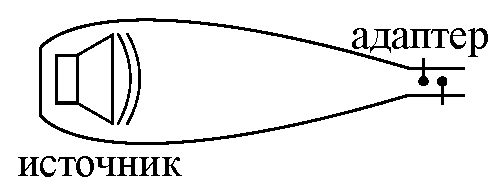
\includegraphics [scale=1] {ris0_2}
	\caption{Схема источника с адаптером для измерения объемной скорости.}
	\label{img:ris0_2}
\end{figure}

Источник представляет собой электродинамическую головку, помещенную в продолговатый пластиковый корпус с узким отверстием (3,75 см). Такая конструкция позволяет создавать акустическое поле, близкое к полю точечного монопольного источника. Адаптер представляет собой пластиковую трубку кругового сечения, плотно пригнанную к выходному отверстию источника. Внутрь трубки помещены два микрофона, сигналы с которых используются для восстановления объемной скорости источника. Для регистрации рассеянного сигнала использовался Bruel\&Kjaer 4957 1/4 inch Array Microphone, характеристики которого близки к характеристикам микрофонов в адаптере.

\section{Выделение импульсного отклика, связанного только с дифракционным процессом}

Как уже было сказано, сигнал $\{ H_k \}$ необходимо очистить, выделив импульсный отклик дифракционного процесса. Заметим, что основные помехи вносятся источником звука OmniSource, в котором происходят многочисленные
переотражения.

Для простоты будем рассматривать дискретные сигналы $\{ A_k \}$ и $\{ H_k \}$ как непрерывные сигналы $A(t)$ и $H(t)$. При этом будем помнить, что Фурье-образы таких сигналов определены для дискретного набора частот. Введем следующие функции:

\begin{enumerate}
	\item $W(t)$ - производная объемной скорости источника по времени при подаче на вход системы сигнала $A(t)$.
	\item $H^{\text{prop}}(t)$ - импульсный отклик, описывающий распространение волны от источника до микрофона (именно он нас и интересует), определяемый соотношением
	\begin{equation}
	p(t) = \frac{\rho_0}{4\pi} \int_{-\infty}^{\infty} W(\tau) H^{\text{prop}}(t-\tau) d\tau,
	\end{equation}
	где $p(t)$ - давление в точке наблюдения при подаче на вход системы сигнала $A(t)$, $\rho_0$ - плотность воздуха.
	\item $H^{\text{recv}}(t)$ - импульсный отклик приемной части (микрофона, усилителя и АЦП), определяемый соотношением
	\begin{equation}
	H(t) = \int_{-\infty}^{\infty} p(\tau) H^{\text{recv}}(t-\tau)d\tau
	\end{equation}
\end{enumerate}

Нормировочный множитель $\rho_0/4\pi$ в формуле, определяющей $H^{\text{prop}}$, введен из следующих соображений. Хорошо известно, что в свободном пространстве точечный монопольный источник создает давление, пропорциональное производной его объемной скорости по времени:

\begin{equation}
p = \frac{\rho_0}{4\pi R} W(t-R/c),
\end{equation}
где $R$ - расстояние от источника до точки наблюдения. Таким образом, в этом случае импульсный отклик $H^{prop}$ представляет собой дельта-функцию (в дискретном случае — одиночный импульс):
\begin{equation}
H^{\text{prop}} = \frac{\delta(t-R/c)}{R}.
\end{equation}

Амплитуда дельта-функции обратно пропорциональна расстоянию до источника $R$ и обращается в единицу при $R = 1$ м, что удобно.
Будем обозначать Фурье-образ сигнала $\zeta(t)$ как $\zeta_\omega$. Тогда для наших сигналов будем иметь:

\begin{eqnarray}
&p_\omega = W_\omega H_\omega^{\text{prop}},\\
&H_\omega = p_\omega H_\omega^{\text{recv}}.
\end{eqnarray}
Если удастся измерить производную по времени объемной скорости источника $W(t)$, то можно будет восстановить дифракционную часть импульсного отклика:

\begin{equation}
\label{eq:mls_main}
H_\omega^{\text{prop}} = \frac{H_\omega}{W_\omega H_\omega^{recv}}.
\end{equation}

Заметим, что предложенная процедура выделения части импульсного отклика, связанной только с дифракционным процессом никак не использует преимуществ метода М-последовательностей. Действительно, и $W_\omega$ и $H_\omega$ пропорциональны спектру входного сигнала, а значит, при любом достаточно широкополосном входном сигнале ~\eqref{eq:mls_main} дает возможность восстановить функцию $H^{\text{prop}}(t)$. Тем не менее, использование М-последовательностей позволяет повысить качество восстановления.

Длительность используемого в эксперименте сигнала \textbf{(4 с)} соответствует более чем 1 км пути, проходимого волной. При этом нас интересуют только первые несколько метров импульсного отклика, а вся остальная его часть является помехой. Чтобы ослабить влияние этой помехи, используем для вычисления Фурье-образов только начальную часть сигналов $H(t)$ и $W(t)$. Длительность этой части следует взять такой, чтобы в нее попала вся существенно ненулевая часть сигнала $W(t)$. В описываемых ниже экспериментах использовались первые 50 м сигналов $H(t)$ и $W(t)$, что соответствует примерно 100 переотражениям в корпусе источника.

\section{Измерение производной объемной скорости источника}

Как было сказано ранее, для измерения объемной скорости источника может быть применен адаптер с двумя микрофонами. Схема используемого адаптера приведена на (Рис. \ref{img:ris0_3}).

\begin{figure}[ht]
	\centering
	\includegraphics [scale=1.2] {ris0_3}
	\caption{Схема адаптера для измерения объемной скорости источника.}
	\label{img:ris0_3}
\end{figure}

Пусть при подаче на вход системы М-последовательности $\{ S_k^{\text{in}} \}$ с микрофонов адаптера после усиления и ЦАП приходят сигналы $\{ S_k^{\text{out, 1}} \}$ и $\{ S_k^{\text{out, 2}} \}$. Пусть $\{ H_k^{\text{1, 2}} \}$ — взаимные корреляции этих сигналов с входным сигналом $\{ S_k^{\text{in}} \}$. Обозначим через $p_{1,2}$ начальные части (первые 50 м) сигналов $H^{1,2}$.

Для вычисления объемной скорости предположим, что внутри адаптера распространяются только поршневые моды. Обоснованность этого предположения обсуждается ниже. При таком предположении для каждой частоты $\omega$ давление в трубке может быть представлено в следующем виде:
\begin{equation}
p_\omega(x) = A^{-ikx} + Be^{ikx},
\end{equation}
где $A$ и $B$ — амплитуды волн, распространяющихся в положительном и отрицательном направлении оси $x$ соответственно. Здесь предполагается гармоническая зависимость от времени вида $e^{i\omega t}$. Измеряются давления $p_1(t)$ и $p_2(t)$ в точках $x = -b$ и $x = -a$ соответственно. Для их Фурье-образов можно записать:

\begin{eqnarray}
\label{eq:twomic}
&p_{1\omega} = A e^{ikb} + Be^{-ikb},\\
&p_{2\omega} = A e^{ika} + Be^{-ika},
\end{eqnarray}
откуда:

\begin{equation}
A = \frac{-p_{1\omega}e^{ikb} + p_{2\omega}e^{ika} }{e^{2ika} - e^{2ikb}}, \quad B = \frac{-p_{1\omega}e^{ik(2a+b)} - p_{2\omega}e^{ik(a+2b)} }{e^{2ika} - e^{2ikb}}.
\end{equation}

Пользуясь уравнением Эйлера, для производной колебательной скорости $v$ получим:

\begin{equation}
\label{eq:eq1_16}
\left(\frac{dv}{dt}\right)_\omega = \frac{ik}{\rho_0} (A e^{-ikx} - Be^{ikx}).
\end{equation}

Для производной по времени объемной скорости источника имеем:

\begin{equation}
\label{eq:proizv_vrem}
W_\omega = i\omega \frac{\pi r^2}{\rho_0 c}(A-B),
\end{equation}
где $r$ — радиус трубки адаптера. Полученная формула дает относительно неплохие результаты, однако вносит заметные фазовые искажения. Причиной этих искажений служит то, что трубка не является достаточно тонкой, а значит, ее конец нельзя считать точечным источником. Используя теорию Вайнштейна об излучении волн из открытого конца волновода \cite{Weinstein1966}, можно получить формулу, подходящую для данного случая. Для этого в ~\eqref{eq:eq1_16} надо заменить $B$ на $-A$, то есть

\begin{equation}
W_\omega = i\omega\frac{2\pi r^2 A}{\rho_0 c}.
\end{equation}

Вычисленная таким образом объемная скорость будет содержать в себе также АЧХ приемных трактов адаптера. В действительности микрофоны в адаптере близки по своим характеристикам к микрофону, используемому для регистрации поля вблизи рассеивателя, а АЧХ усилителей в приемных трактах близки к идеальным в интересующем нас диапазоне частот (можно
считать, что $H_\omega^{\text{recv}} = 1$). Формула ~\eqref{eq:mls_main} может быть переписана следующим образом:

\begin{equation}
H_\omega = W_\omega H_\omega^{\text{prop}}.
\end{equation}

Рассмотрим ограничения предлагаемого метода. Очевидной трудностью является то, что формулы \label{eq:twomic} имеют смысл только для частот $f < f_c$, где граничная частота $f_c$ определяется расстоянием между микрофонами: $f_c = c_0/(2(b-a))$. Это частота, при которой знаменатель в \label{eq:twomic} обращается в нуль. В нашем случае \textbf{$f_c = 8.57$} кГц. Таким образом, все сигналы при обработке должны быть пропущены через ФНЧ. 

Другие трудности связаны с модами высших порядков, распространяющимися в трубке адаптера. Эти моды могут влиять на результат двумя способами. Во-первых, они могут излучать звук вовне. Во-вторых, они могут создавать сигнал на микрофонах адаптера, внося ошибки в измерение объемной скорости. Моды высших порядков имеют следующую структуру:

\begin{equation}
p(x, \xi, \varphi) = \exp\{\pm i \gamma x \}\begin{Bmatrix}
\sin(n\varphi) \\
\cos(n\varphi) \\
\end{Bmatrix} J_n(k_{m,n}\xi),
\end{equation}
где $(x, \xi, \varphi)$ — цилиндрические координаты с осью, совпадающей с осью трубки адаптера, $J_n$ — функции Бесселя, $k_{m,n}$ — корни уравнения $J'_n(k_{m,n} r) = 0$, а $\gamma = \sqrt{\omega^2/c_0^2 - k_{m,n}^2}$. Если точка наблюдения расположена вблизи оси системы, что соответствует нашему случаю, то, в силу ортогональности, моды высших порядков не будут давать вклада в излучаемое поле. Все моды, кроме поршневой, имеют свои частоты отсечки, что позволяет оценить их постоянные затухания. Моды с номером $n\neq 0$ не будут влиять на сигналы микрофонов адаптера, поскольку микрофоны расположены на оси трубки, $J_n(0) = 0$ при $n \neq 0$. Поэтому наиболее «опасной»модой будет мода с $J_0(k_{1,0}\xi)$. Простой анализ показывает, что частота отсечки этой моды близкак 11.1 кГц. Для частоты сигнала 5 кГц это соответствует чисто мнимому значению $\gamma = 180i$ $\text{м}^{-1}$. При такой постоянной распространения волна быстро затухает. Таким образом, для частот ниже 5 кГц моды высших порядков можно не рассматривать.

\section{Фильтрация}

Все представленные ниже дифракционные импульсные отклики подвергались фильтрации. Использовалась комбинация фильтров высоких и низких частот со следующими частотными характеристиками. Для ФНЧ:

\begin{equation}
K_{LPF}(f) = \frac{K_0}{2} \left[1 - \text{th} \left(\frac{|f| - f_0}{\Delta f}\right)\right];
\end{equation}

Для ФВЧ:

\begin{equation}
K_{HPF}(f) = K_0 - K_{LPF}(f).
\end{equation}

При этом для фильтра низких частот параметры $f_0$ и $\Delta f$ имели значения $f_0 = 4000$ Гц, $\Delta f$ = 1000 Гц, 
а для фильтра высоких частот $f_0 = 50$ Гц, $\Delta f = 10$ Гц. Нормировочный коэффициент $K_0$ выбирался таким образом, чтобы значение импульсной характеристики результирующего фильтра в нуле было единицей. 

Импульсная характеристика фильтра представлена на Рис. \ref{img:ris0_4}.

\section{Измерения в пустом полупространстве}

Простейшим акустическим окружением, легко реализуемым в эксперименте, является пустое полупространство с жесткой границей. Давление в точке наблюдения в этом случае создается прямой полной и волной, отраженной
от границы полупространства. Импульсный отклик $H^{\text{prop}}$ имеет вид

\begin{equation}
\label{eq:hprop}
H^{\text{prop}} = \frac{\delta(t - R/c)}{R} + \frac{\delta(t - \bar{R}/c)}{\bar{R}},
\end{equation}
где $R$ и $\bar{R}$ — расстояния от точки наблюдения до источника и до отражения источника в границе полупространства соответственно. 

\begin{figure}[ht]
	\centering
	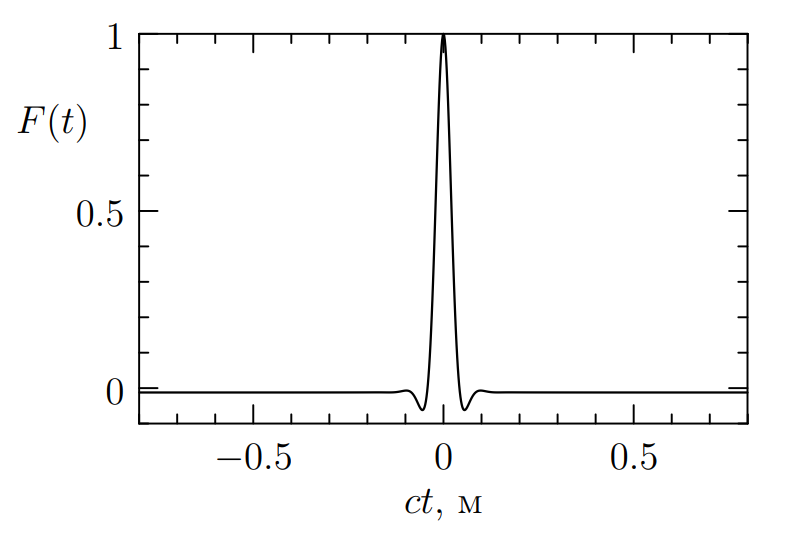
\includegraphics [scale=0.6] {ris0_4}
	\caption{Импульсная характеристика используемого фильтра.}
	\label{img:ris0_4}
\end{figure}

Для проверки работоспособности методики был проведен эксперимент, схема которого показана на (Рис. \ref{img:ris0_5}).

\begin{figure}[ht]
	\centering
	\includegraphics [scale=0.7] {ris0_5}
	\caption{Схема измерений в пустом полупространстве.}
	\label{img:ris0_5}
\end{figure}

Все окружающие предметы были удалены на такое расстояние, чтобы отраженные от них волны приходили на микрофон позже прямой и отраженной от пола волн. Указанное на (Рис. \ref{img:ris0_5}) расположение источника и микрофона соответствует значениям $R = 1$ м и $\bar{R} \approx 4.5$ м. 

В соответствии с ~\eqref{eq:hprop} в импульсном отклике мы должны увидеть две копии импульсной характеристики использованного фильтра (Рис. \ref{img:ris0_4}), сдвинутые в положения $ct = 1$ м и $ct = 4.5$ м. При этом амплитуда первого пика должна быть равна единице, а второго $1/4.5 \approx 0.22$. На (Рис. \ref{img:ris0_6}) показан наблюдаемый в эксперименте импульсный отклик пустого полупространства.

\begin{figure}[ht]
	\centering
	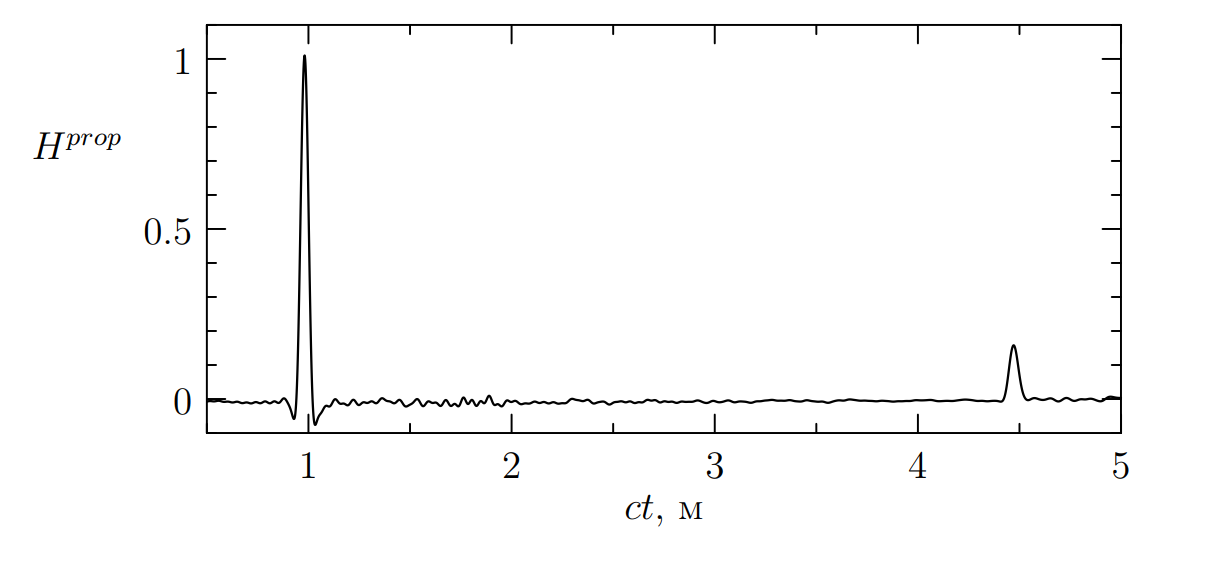
\includegraphics [scale=0.55] {ris0_6}
	\caption{Измеренный импульсный отклик пустого полупространства.}
	\label{img:ris0_6}
\end{figure}

Хорошо видно, что пики имеют правильные положения и что высота первого пика также верна. Высота второго пика несколько ниже предсказанной теоретически, что, по видимому, объясняется неравномерностью диаграммы
направленности использованного источника.

Для иллюстрации роли всех этапов обработки сигнала рассмотрим показанный на (Рис. \ref{img:ris0_7}) импульсный отклик $H^{\text{prop}}$, восстановленный без использования вайнштейновской поправки ~\eqref{eq:proizv_vrem} и импульсный отклик всей системы $H$ (Рис. \ref{img:ris0_8}).

\begin{figure}[ht]
	\centering
	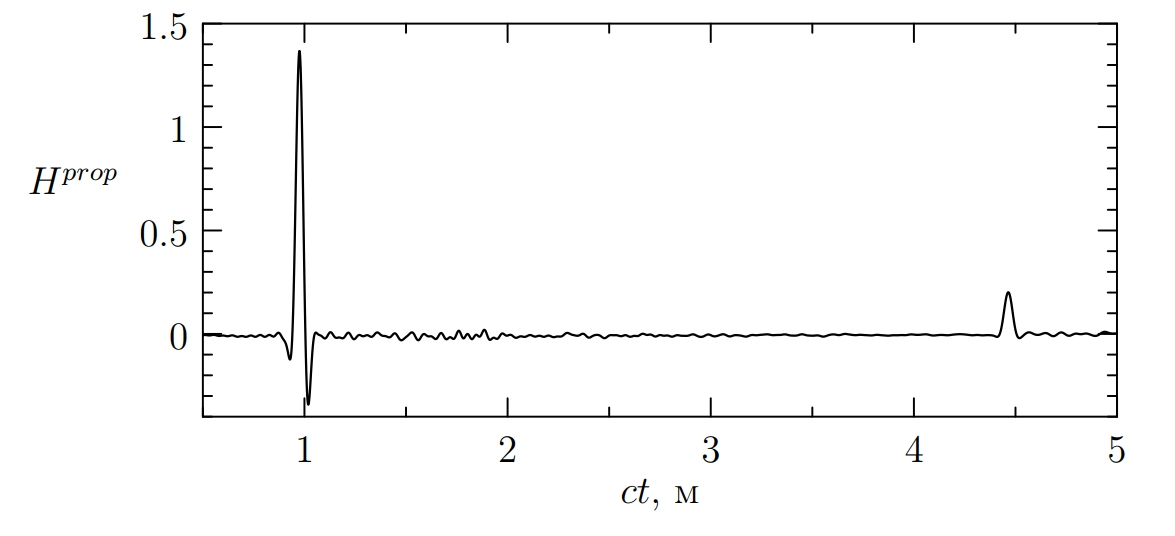
\includegraphics [scale=0.55] {ris0_7}
	\caption{Отклик, восстановленный без использования вайнштейновской поправки.}
	\label{img:ris0_7}
\end{figure}

\begin{figure}[ht]
	\centering
	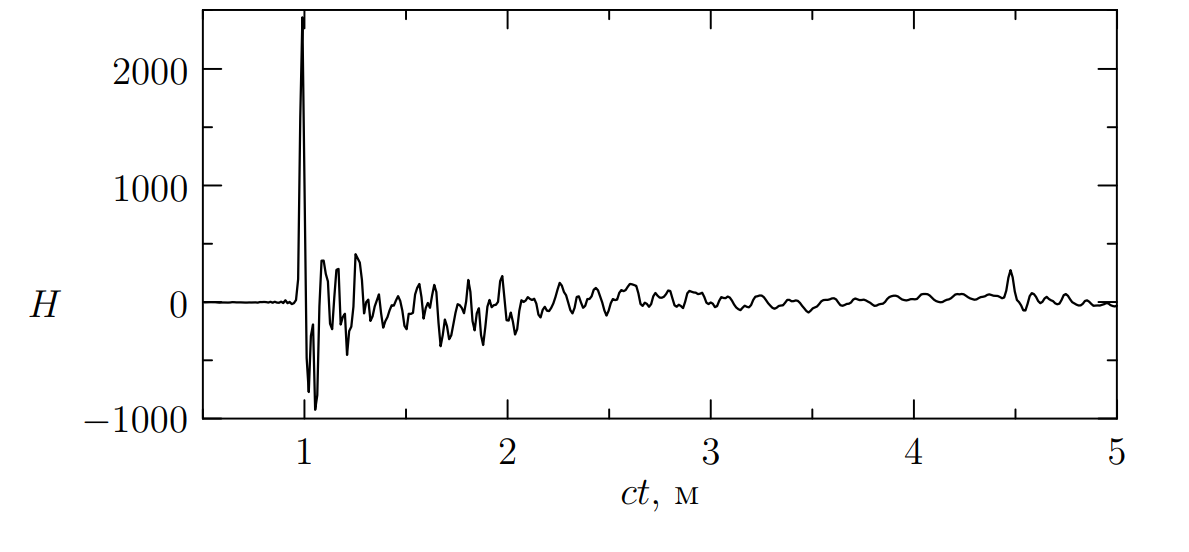
\includegraphics [scale=0.55] {ris0_8}
	\caption{Импульсный отклик всей системы при измерении в пустом полупространстве.}
	\label{img:ris0_8}
\end{figure}

Хорошо видно, что без использования вайнштейновской поправки в восстанавливаемый импульсный отклик вносятся заметные амплитудные и фазовые искажения. В полном импульсном отклике $H$ видны многократные переотражения
внутри источника, делающие сигнал непригодным для анализа.           % Глава про MLS эксперимент
\chapter{Экспериментальная оценка частотной зависимости коэффициента отражения звукопоглощающего материала при наклонном падении}

\section{Введение}
Задача экспериментального измерения коэффициента отражения (поглощения) материалов является одной из важнейших в архитектурной акустике. Классическим методом измерения звукопоглощения является метод, основанный на измерении времени реверберации в реверберационной камере \cite{Blauert} с помещенным в нее исследуемым материалом. Форма камеры подбирается таким образом, чтобы звуковое поле в ней имело диффузный характер. На основе формулы Сэбина вычисляется интегральная оценка коэффициента отражения исследуемого материала. Результатом становится оценка частотной зависимости коэффициента отражения в диффузном поле. Данный метод требует постройки дорогих сооружений и принципиально неточен, поскольку предположения, сделанные при получении реверберационной формулы, недостижимы на практике \cite{Kosten}. Другим классическим методом является метод импедансной трубы, также называемой акустическим интерферометром. Метод импедансной трубы вариативен: в качестве входного сигнала можно использовать монохроматический \cite{Beranek} или широкополосный \cite{ASTM} сигнал; один \cite{Fahy1984}, два \cite{Seybert} или более \cite{Chung1980I, Chung1980II} микрофонов для измерения давления в трубе; также существует множество техник обработки результатов эксперимента \cite{Chu1991}. Но результатом измерения может стать только частотная зависимость коэффициента отражения при нормальном падении.

Эти методы годятся для исследования свойств материала, но их нельзя использовать на месте при натурных измерениях, например, в помещении, где материалы уже смонтированы. Настоящие натурные измерения возможны только при исследовании амплитуды акустического поля, отраженного от уже смонтированного материала. Подробный обзор методов измерения коэффициента поглощения и импеданса при этих измерениях приведен в \cite{Brandao2015}. Первыми такую технику применили Ингард и Болт \cite{Ingard1951} и Андо \cite{Ando1968} с монохроматическим сигналом в заглушенной камере. Наиболее простые подобные техники не позволяют измерить угловую зависимость коэффициента отражения и используют монохроматические сигналы, что увеличивает время измерения \cite{Yuzawa1975}. В процессе развития техники начали использоваться импульсные сигналы \cite{Davies1979, Kintzl}. Их использование позволило лучше разрешить отраженный сигнал от падающего по времени. Создание стабильного импульсного во времени источника с идеальной повторяемостью, а также защита микрофона от повреждения импульсным сигналом представляют сложную техническую проблему. Холлин и Джонс использовали корреляцию между шумовым сигналом, излучаемым источником, и сигналом, принимаемым микрофоном, чтобы избавиться от паразитных шумов \cite{Hollin1977}. 

В работе \cite{Garai1993} отмечены недостатки использования импульсных источников звука (плохая повторяемость, нелинейность и сложность обработки экспериментальных данных). В \cite{Garai1993} измеряется импульсный отклик исследуемого материала при помощи метода последовательностей максимальной длины только при нормальном падении. Прямой и отраженный сигнал в импульсном отклике вырезались с помощью гладкой оконной функции, исследовалось влияние формы оконной функции. Затем получалась частотная зависимость коэффициента отражения с помощью Фурье-преобразования от вырезанного фрагмента. 

В \cite{Garai1993} в качестве источника используется маленький динамик. Использование такого источника приводит к необходимости подбирать динамик с ровной в широком диапазоне частотной характеристикой, чтобы импульсный отклик был узким во временной области, и было возможно разрешить часть импульсного отклика, соответствующую отражению от исследуемого материала. Динамик кроме ровной частотной характеристики должен иметь небольшие размеры, чтобы он мог считаться точечным источником. Кроме того, он должен иметь мощность, достаточную для того, чтобы сигнал не затух по пути до приемника. А для справедливости оценки коэффициента отражения как отношения отраженного поля к падающему нужно считать падающее поле полем плоской волны. Для чего следует располагать точечный источник на значительном расстоянии от исследуемого материала. Поэтому такой подбор может быть сложным. Данная работа лишена такого недостатка, поскольку используется монопольный источник на основе мощного динамика большого диаметра, а объемная скорость на выходе из источника измеряется при помощи метода двух микрофонов, и частотная характеристика динамика не влияет на результат. 
	
Техника, описанная в \cite{Garai1993}, была развита и использована для измерения коэффициента поглощения при наклонном падении \cite{Mommertz1995}. Существует также техника измерения коэффициентов отражения при наклонном падении, основанная на двумерном пространственном Фурье-преобразовании сигналов, измеренных в двух параллельных плоскостях, лежащих близко к поверхности испытуемого материала \cite{Tamura1990I, Tamura1990II}. 
	
В настоящей работе предлагается техника экспериментального определения частотной зависимости коэффициента отражения при падении под углом, основанная на анализе импульсного отклика исследуемого материала. Измерения ведутся с помощью монопольного источника, выполненного из динамика и конусовидного концентратора. Восстановление угловой зависимости производится посредством обращения интеграла Фурье-Бесселя. Исследовано отличие коэффициента отражения, вычисленного при помощи деления спектра отраженного поля на спектр падающего поля, с коэффициентом отражения, вычисленным при помощи обращения этого интеграла. Проверка новой техники производится на хорошо исследованном звукопоглощающем материале – вспененном меламине. Этот материал представляет собой вспененный пластик на основе полимера меламин-формальдегидной смолы и описывается известной математической моделью Био \cite{Biot1956_I, Biot1956_II}. Материал используется для тепло- и звукоизоляции. Свойства вспененного меламина хорошо известны и измерены в ряде работ \cite{Geebelen2007, Cuenca2014}. В данной работе используется псевдошумовой сигнал, что позволяет получить импульсный отклик, не сталкиваясь с техническими проблемами, связанными с использованием импульсного источника. Отраженный сигнал выделяется из импульсного отклика при помощи умножения отклика на гладкую оконную функцию, аналогично \cite{Garai1993}. Главным недостатком предлагаемой в данной работе техники можно считать необходимость тщательной сравнительной калибровки используемых микрофонов. Эта сложность может быть преодолена, если вместо трех микрофонов использовать один микрофон, повторяя эксперимент для каждого его расположения (два положения в адаптере измерения объемной скорости и одно в точке наблюдения).

\section{Постановка задачи}

Исследуемый материал занимает область  $-H < z < 0$  декартовой системы координат $(x,y,z)$. Область $z > 0$ занята воздухом, на $z = -H$ находится акустически твердая стенка (Рис. \ref{img:ris1_1}). 

\begin{figure}[ht]
	\centering
	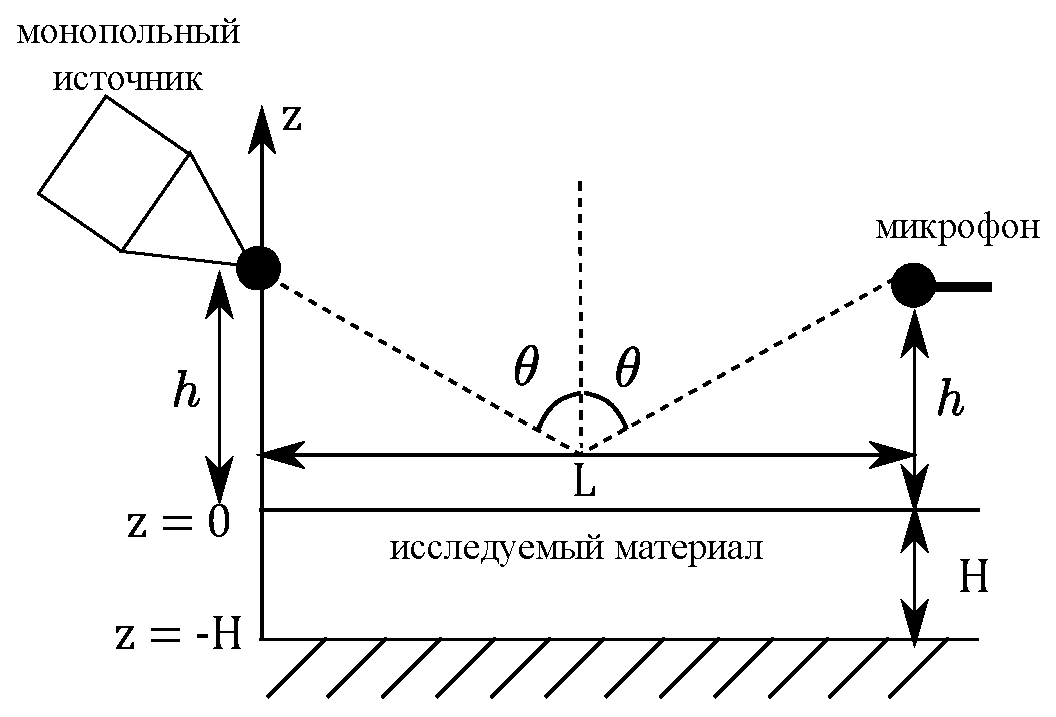
\includegraphics [scale=0.8] {ris1_1}
	\caption{Схема эксперимента.}
	\label{img:ris1_1}
\end{figure}

Акустические волны в среде возбуждает монопольный источник, находящийся в точке $(0, 0, h), h > 0$. Приемник расположен в точке  $(L, 0, h)$.
 
Поле точечного источника опишем неоднородным волновым уравнением
\begin{equation}
\label{eq:waveequation}
\frac{1}{c_0^2} \frac{\partial^2 p}{\partial t^2} - \Delta p = \rho_0 \frac{\partial W(t)}{\partial t} \delta(x) \delta(y) \delta(z-h),
\end{equation}
где $W(t)$ – объем воздуха, производимого в единицу времени источником, измеряется в $\text{м}^3$/\text{с}; $c$ - скорость звука в воздухе.

В эксперименте измеряется набор импульсных откликов для углов падения $\theta_n$. Из каждого импульсного отклика при помощи преобразования Фурье вычисляется частотная характеристика $P_n(\omega)$ отраженного от образца поля для каждого угла падения $\theta_n$. При обработке из частотных характеристик получается частотная зависимость коэффициента отражения от образца при данном угле падения.

\section{Описание поля сферической волны. Интеграл Фурье-Бесселя}

Рассмотрим стационарную задачу распространения гармонической волны с частотой $f$. В этом случае $W(t) = Be^{-i\omega t}$, $\omega = 2\pi f$. Экспоненциальная зависимость всех величин от времени будет далее опущена. Решение стационарной задачи будет представлять собой сумму прямого и отраженного поля:

\begin{equation}
P = P_d + P_r.
\end{equation}

Прямое поле $P_d$ на приемнике вычисляется по формуле монопольного источника \cite{Isakovich1973}:

\begin{equation}
\label{eq:pointsource}
P_d(\omega, r) = - \frac{i\omega\rho_0 \exp{i k_0 L}}{4 \pi r} w(\omega),
\end{equation}
где $w(\omega)$ - Фурье-образ $W(t)$, $k_0 = \omega / c_0$, $\omega = 2 \pi f$.

Отраженное поле дается интегралом Фурье-Бесселя \cite{Biot1956_I, Biot1956_II}:

\begin{multline}
\label{eq:reflectedfield}
P_r(\omega, 2h, L) = w(\omega) \frac{\omega \rho_0}{4 \pi} \int_{0}^{\infty} \frac{k_{||} R(\omega, \arcsin(k_{||}/k_0) ) J_0(k_{||}L)}{\sqrt{k_0^2 - k_{||}^2}} \\
 \exp(i \sqrt{k_0^2 - k_{||}^2} 2h) dk_{||},
\end{multline}  
где $k_{||} = k_0 \sin\varphi$ – величина проекции волнового вектора на плоскость $Oxy$, $\varphi = \arcsin\left(\frac{k_{||}}{k_0}\right)$, $R$ – коэффициент отражения плоской волны, падающей под углом к нормали $\varphi = \arcsin(k_{||}/k_0)$. Коэффициент отражения определяется свойствами материала и его толщиной. В настоящей работе исследуется вспененный меламин, который описывается моделью Био для пористых сред \cite{Biot1956_I, Biot1956_II}. Для материалов, которые описываются этой моделью, было получено аналитическое выражение для коэффициента отражения в \cite{Allard2009}.

В эксперименте непосредственно измеряется полное поле $P = P_r + P_d$ для разных положений источника и приемника. Затем путем обработки из него выделяется величина $P_r$, из нее строится оценка для коэффициента отражения. Простейшая оценка коэффициента отражения может быть получена путем деления $P_r$ на поле монопольного источника ~\eqref{eq:pointsource}. Такая оценка, очевидно, будет справедлива только в том случае, когда источник находится достаточно далеко от поверхности исследуемого материала. Действительно, в этом случае поле излучаемое источником близко к полю плоской волны, которое отражается с коэффициентом, близким к $R$. Оценим с помощью формулы ~\eqref{eq:reflectedfield} точность такой оценки для случая нормального падения. Учитывая, что $J_0(0) = 1$, и оценивая оставшийся интеграл с помощью метода перевала, получим:
  		
\begin{multline}
\label{eq:reflectedfield2}
P_r(\omega, 2h, 0) = R(\omega, 0) P_d(\omega, 2h) + P_d(\omega, 2h) R'(\omega, 0) \sqrt{\frac{\pi i}{2k_0(2h)}} +  \\
O([k_0(2h)]^{-2}),
\end{multline}
где штрих обозначает частную  производную по второму аргументу. В эксперименте $2h \sim 1$  м, следовательно, оценка коэффициента отражения по первому члену в ~\eqref{eq:reflectedfield2} будет справедлива на частотах выше 500 Гц. Кроме того, второй член в ~\eqref{eq:reflectedfield2} позволяет апостериорно оценить корректность аппроксимации путем вычисления производной $R'$.



\section{Отыскание коэффициента отражения с помощью обращения интеграла Фурье-Бесселя}

Более точная оценка для коэффициента отражения может быть построена с помощью приближенного обращения интеграла Фурье-Бесселя. Переходя от переменной $k_{||}$ к переменной $\varphi = \arcsin\left(\frac{k_{||}}{k_0}\right)$ в ~\eqref{eq:reflectedfield}, получим:

\begin{equation}
\label{eq:fb_change_vars}
\tilde{P}_r(\omega, \theta, h) = w(\omega) \frac{\omega \rho_0}{4 \pi} \int_{\Gamma} k_0 \sin \varphi R(\omega, \varphi) J_0\left(\frac{2 k_0 h \sin \varphi}{\tan \theta}\right) e^{2 i k_0 h \cos \varphi} d \varphi,
\end{equation}
где $\tilde{P}_r(\omega, \theta, h) = P_r(\omega, 2h, \frac{2h}{\tan \theta})$, а контур $\Gamma$ изображен на (Рис. \ref{img:ris1_2}). Пусть из эксперимента известен набор функций $P_n = \tilde{P}_r(\omega, \theta_n, h)$ при заданных $\theta_n$, $1\leq n \leq N$. В интеграле ~\eqref{eq:fb_change_vars} заменим $R(\varphi)$ на некоторую интерполяцию 
\begin{equation}
\label{eq:reflectionsum}
\tilde{R}(\omega, \varphi) = \sum_{m=1}^{N} R_m(\omega) E_m(\varphi),
\end{equation}
где $E_m$ – интерполяционные функции, а $R_m(\omega)$ – функции, подлежащие определению. Подставляя ~\eqref{eq:reflectionsum} в ~\eqref{eq:fb_change_vars} и проводя интегрирование, получим следующее матричное уравнение: 
\begin{equation}
\label{eq:mainequation}
P_n = M_{nm}R_m,
\end{equation}
где
\begin{equation}
\label{eq:Mnm}
M_{nm} = w(\omega) \frac{\omega \rho_0}{4 \pi} \int_{\Gamma} k_0 \sin\varphi E_m(\varphi) J_0\left(\frac{2k_0 h \sin\varphi}{\tan\theta_n}\right) e^{2ik_0 h \cos \varphi} d\varphi.
\end{equation}

\begin{figure}[ht]
	\centering
	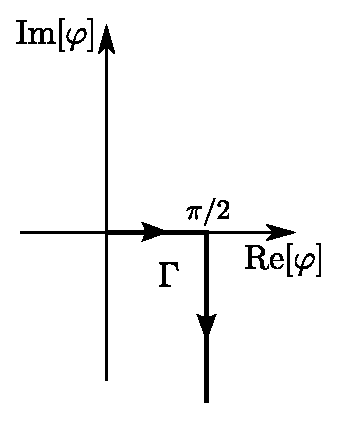
\includegraphics [scale=1] {ris1_2}
	\caption{Контур интегрирования.}
	\label{img:ris1_2}
\end{figure}

Решая уравнение ~\eqref{eq:mainequation}, определим неизвестные коэффициенты $R_m$ и, пользуясь формулой ~\eqref{eq:reflectionsum}, получим оценку для коэффициента отражения. Корректность построенной оценки сильно зависит от выбранных интерполяционных функций. Если на заданном наборе $\theta_n$ коэффициент отражения меняется плавно, то на участке $[0; \pi/2]$ функции $E_n$ могут быть выбраны кусочно-линейными:

\begin{equation}
\label{eq:shapefunctions}
E_n(\varphi)=
\begin{cases}
0, \varphi \leq \theta_{n-1}, \varphi \geq \theta_{n+1} \\
\dfrac{\theta_{n+1} - \varphi}{\theta_{n+1} - \theta_n}, \theta_n < \varphi < \theta_{n+1} \\
\dfrac{\varphi - \theta_n}{\theta_{n+1} - \theta_n}, \theta_{n-1} < \varphi < \theta_n
\end{cases}
\end{equation}

Отметим, что если $E_n$ выбраны в соответствии с ~\eqref{eq:shapefunctions}, то коэффициенты $R_m(\omega)$ являются приближением к коэффициенту отражения $R(\omega, \theta_m)$ .

Остановимся на деталях численной реализации. 

Важной задачей является выбор последней функции $E_n(\varphi)$ при мнимых $\varphi$. В данной работе $E_n(\varphi) = 1, \text{Im}[\varphi] < 0$ . Данный выбор был обусловлен следующими соображениями. При $h \neq 0$ такой выбор слабо влияет на результат ввиду экспоненциального затухания подынтегрального выражения в ~\eqref{eq:Mnm}. Однако при $h = 0$, когда быстрого затухания нет, получается постоянный коэффициент отражения при мнимых углах, что соответствует модели Био (при касательном падении меламин ведет себя как граница Дирихле).

Хорошо известно, что задача решения уравнения 

\begin{equation}
R_m = M_{nm}^{-1} P_n
\end{equation}
является некорректно поставленной, так как матрица $M_{nm}$ плохо обусловлена, и непосредственное ее численное обращение может вести к значительным численным ошибкам. Поэтому при решении уравнения ~\eqref{eq:mainequation} применялась регуляризация Тихонова

\begin{equation}
R_m = (M_{nm}^T M_{nm} + \lambda I)^{-1} M_{nm}^{-1} P_n,
\end{equation}
где $I$ - единичная матрица, а параметр $\lambda$ выбирался исходя из численных экспериментов. На частотах от $500$ до $2000$ Гц выбиралось значение $\lambda = 0.2$, на более высоких частотах регуляризация не требовалась.

\section{Описание эксперимента}

Геометрия эксперимента соответствует Рис. ~\ref{img:ris1_1}. Параметры $h$ и $L$ подбирались таким образом, чтобы расстояние, проходимое отраженным сигналом, было порядка 1 метра.

\begin{figure}[ht]
	\centering
	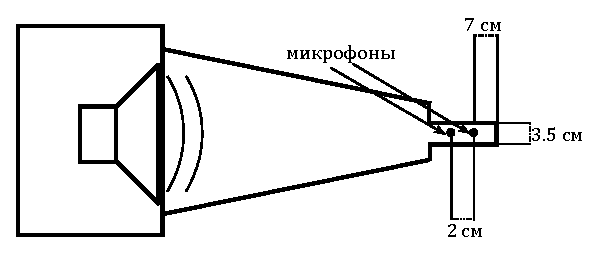
\includegraphics [scale=1] {ris1_3}
	\caption{Схема монопольного источника.}
	\label{img:ris1_3}
\end{figure}

В качестве монопольного источника использовался аналог Bruel \& Kjaer 4295 Omnisource, выполненный из фанерного короба с клиновидным концентратором (Рис. \ref{img:ris1_3}). К источнику крепится адаптер для измерения объемной скорости. Адаптер представляет собой отрезок металлической трубы диаметром $3,5$ см с двумя отверстиями для микрофонов, расстояние между которыми $2$ см. Это расстояние определяет наивысшую частоту, для которой возможно определение колебательной скорости ($8,5$ кГц). Это ограничение следует из метода двух микрофонов \cite{ASTM}. Для регистрации поля и измерения объемной скорости использовались $6$ мм микрофоны Audix TM1, обладающие достаточно ровной частотной характеристикой в широком диапазоне частот. 
	
Импульсный отклик определялся с помощью метода \textit{M}-последовательности. Подробно данная техника описана в \cite{ValyaevMLS}. Остановимся здесь лишь на основных моментах. \textit{M}-последовательность – это двухуровневый квазишумовой сигнал с количеством отсчетов $2^M - 1$, где для данной работы $M = 19$ (длительность около $11$ секунд с частотой дискретизации $48$ кГц). \textit{М}-последовательность подается на ЦАП и воспроизводится источником. Затем принимаются сигнал с микрофона, расположенного в точке приема и пара сигналов  с двух микрофонов, помещенных в адаптер объемной скорости. Вычисляется кросс-корреляция каждого из сигналов с исходной \textit{M}-последовательностью. На корреляционные функции накладывается временное окно, чтобы выделить первые несколько метров принятого сигнала и отрезать весь остальной сигнал. Затем с каждым из сигналов производится преобразование Фурье. Из сигналов, полученных с микрофонов в адаптере, вычисляется Фурье-спектр объемной скорости при помощи формулы двух микрофонов с учетом поправки Вайнштейна, описывающей отражение от открытого конца волновода \cite{Weinstein1966}. Отношение спектра давления в точке приема к спектру объемной скорости источника дает частотный отклик всего акустического тракта. 
	
Далее выполняется фильтрация фильтром низких частот с частотой отсечки $4500$ Гц и шириной $500$ Гц. Фильтрация позволяет избежать импульсов с большими пиковыми величинами. Для удобства результат нормируется таким образом, чтобы амплитуда пика от прямого сигнала была единичной при расстоянии от источника до микрофона $1$ м. После фильтрации к полученному сигналу применяется обратное преобразование Фурье. Обратное преобразование Фурье дает профильтрованный импульсный отклик. 

Поскольку эксперимент имел хорошую повторяемость, была возможность улучшить соотношение сигнал/шум, вычитая из отклика, полученного при наличии отражения от исследуемого материала, отклик свободного поля без материала. Сначала проводился эксперимент с отражением от исследуемого материала Рис. ~\ref{img:ris1_4}, линия из точек. Затем исследуемый материал и жесткая подложка убирались, и импульсный отклик измерялся снова. Так получался отклик свободного поля, который вычитался из отклика, полученного с отражением от материала, и так повышалось отношение амплитуд сигнала и шума в отклике Рис. ~\ref{img:ris1_4}, сплошная линия. Из полученного таким образом импульсного отклика при помощи гладкой маски (Рис. ~\ref{img:ris1_4}, пунктирная линия) вырезается часть, соответствующая отраженному сигналу. Фурье-образ вырезанной части представляет собой отраженное поле $P_r$.

\begin{figure}[ht]
	\centering
	\label{img:ris1_4}
	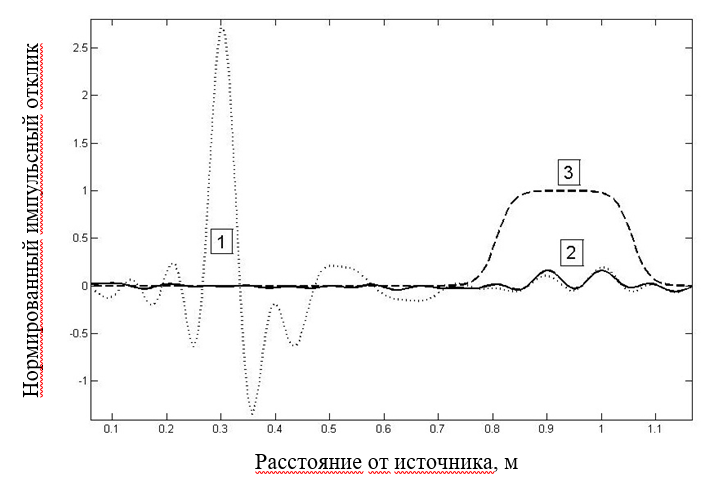
\includegraphics [scale=0.75] {ris1_4}
	\caption{Пример импульсного отклика. По горизонтальной оси отложено расстояние от источника, по вертикальной оси отложена амплитуда импульсного отлика. Линия из точек соответствует сигналу до вычитания отклика свободного поля; сплошная линия – сигналу после вычитания; пунктирная линия – маске, необходимой для выделения участка, соответствующего отражению от меламина. Пик 1 соответствует прямому сигналу от источника; пара пиков 2 соответствует сигналу, отраженному от меламина (один пик от поверхности меламина, другой от подложки, на которую он наклеен); маска 3 предназначена для выделения отраженного сигнала.}
\end{figure}

Проводится серия таких экспериментов для разных углов падения $\theta$. С помощью методов, описанных в предыдущем разделе, строится оценка для коэффициента отражения.

\section{Экспериментальные результаты}

Для проверки работоспособности предлагаемой методики и построенной экспериментальной установки были проведены эксперименты по измерению импульсного отклика исследуемого материала с углами $\theta = 0 ^{\circ}, 15 ^{\circ}, 30 ^{\circ}, 45 ^{\circ}, 60 ^{\circ}$ (см. Рис. ~\ref{img:ris1_1}). Из модели Био известно, что с изменением угла $\theta$ величина коэффициента отражения меняется плавно, поэтому такого небольшого набора углов должно быть достаточно. К сожалению, измерения для больших углов $\varphi$ были затруднены ввиду наложения прямого и отраженного сигнала в импульсном отклике. К тому же, имелись проблемы, связанные с конечным размером образца: на низких частотах образец оказывается меньше размера первой зоны Френеля, и тогда, если расстояние от источника до образца около $0,5$ м, сторона образца должна быть около $1,5$ м. 
	
После окончания измерений получается набор частотных характеристик $P_n = \tilde{P}_r(\omega, \theta_n, h)$ для каждого угла падения $\theta_n$. После того, как по формулам ~\eqref{eq:reflectedfield2} и ~\eqref{eq:reflectionsum}, ~\eqref{eq:mainequation} были получены оценки для коэффициента отражения, они сравнивались с такой же зависимостью, вычисленной по модели Био с учетом толщины образца при помощи переходной матрицы. Метод вычисления теоретической зависимости описан в \cite{Allard2009}.

\begin{figure}[ht]
	\centering
	\label{img:ris1_5}	
	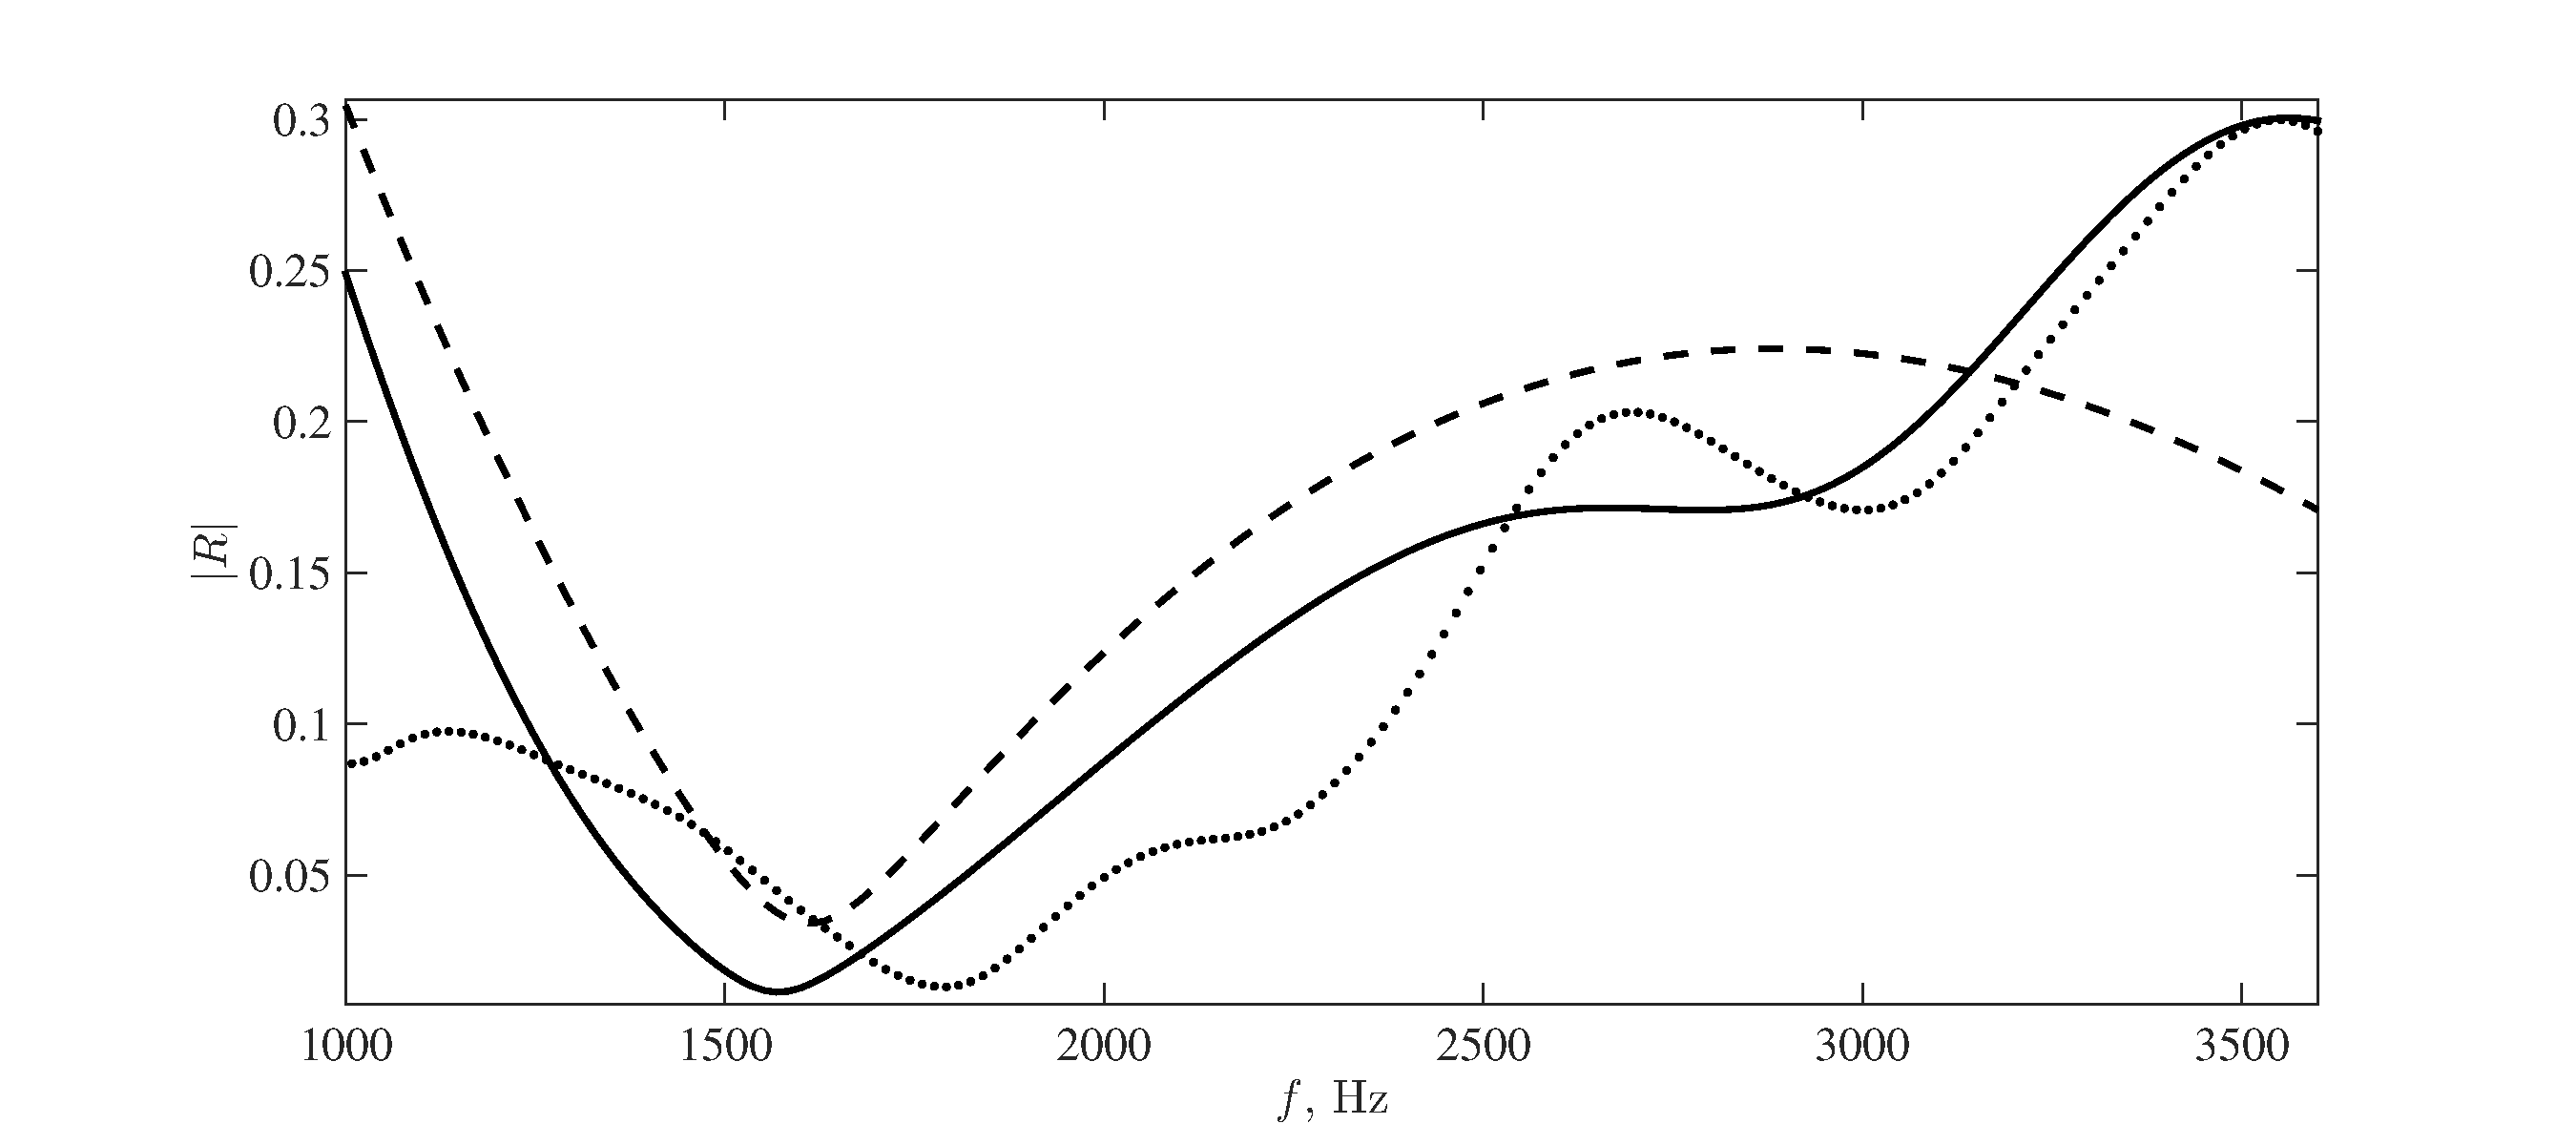
\includegraphics [scale=0.4] {ris1_5}
	\caption{График зависимости модуля коэффициента отражения $|R|$ при угле падения равном $0^\circ$. Пунктирной линией обозначен результат, полученный с помощью формулы ~\eqref{eq:reflectedfield2}, точками – с помощью формул ~\eqref{eq:reflectionsum}, ~\eqref{eq:mainequation}, сплошной линией – результат теоретического расчета на основе модели Био.}
\end{figure}

\begin{figure}[ht]
	\centering
	\label{img:ris1_6}	
	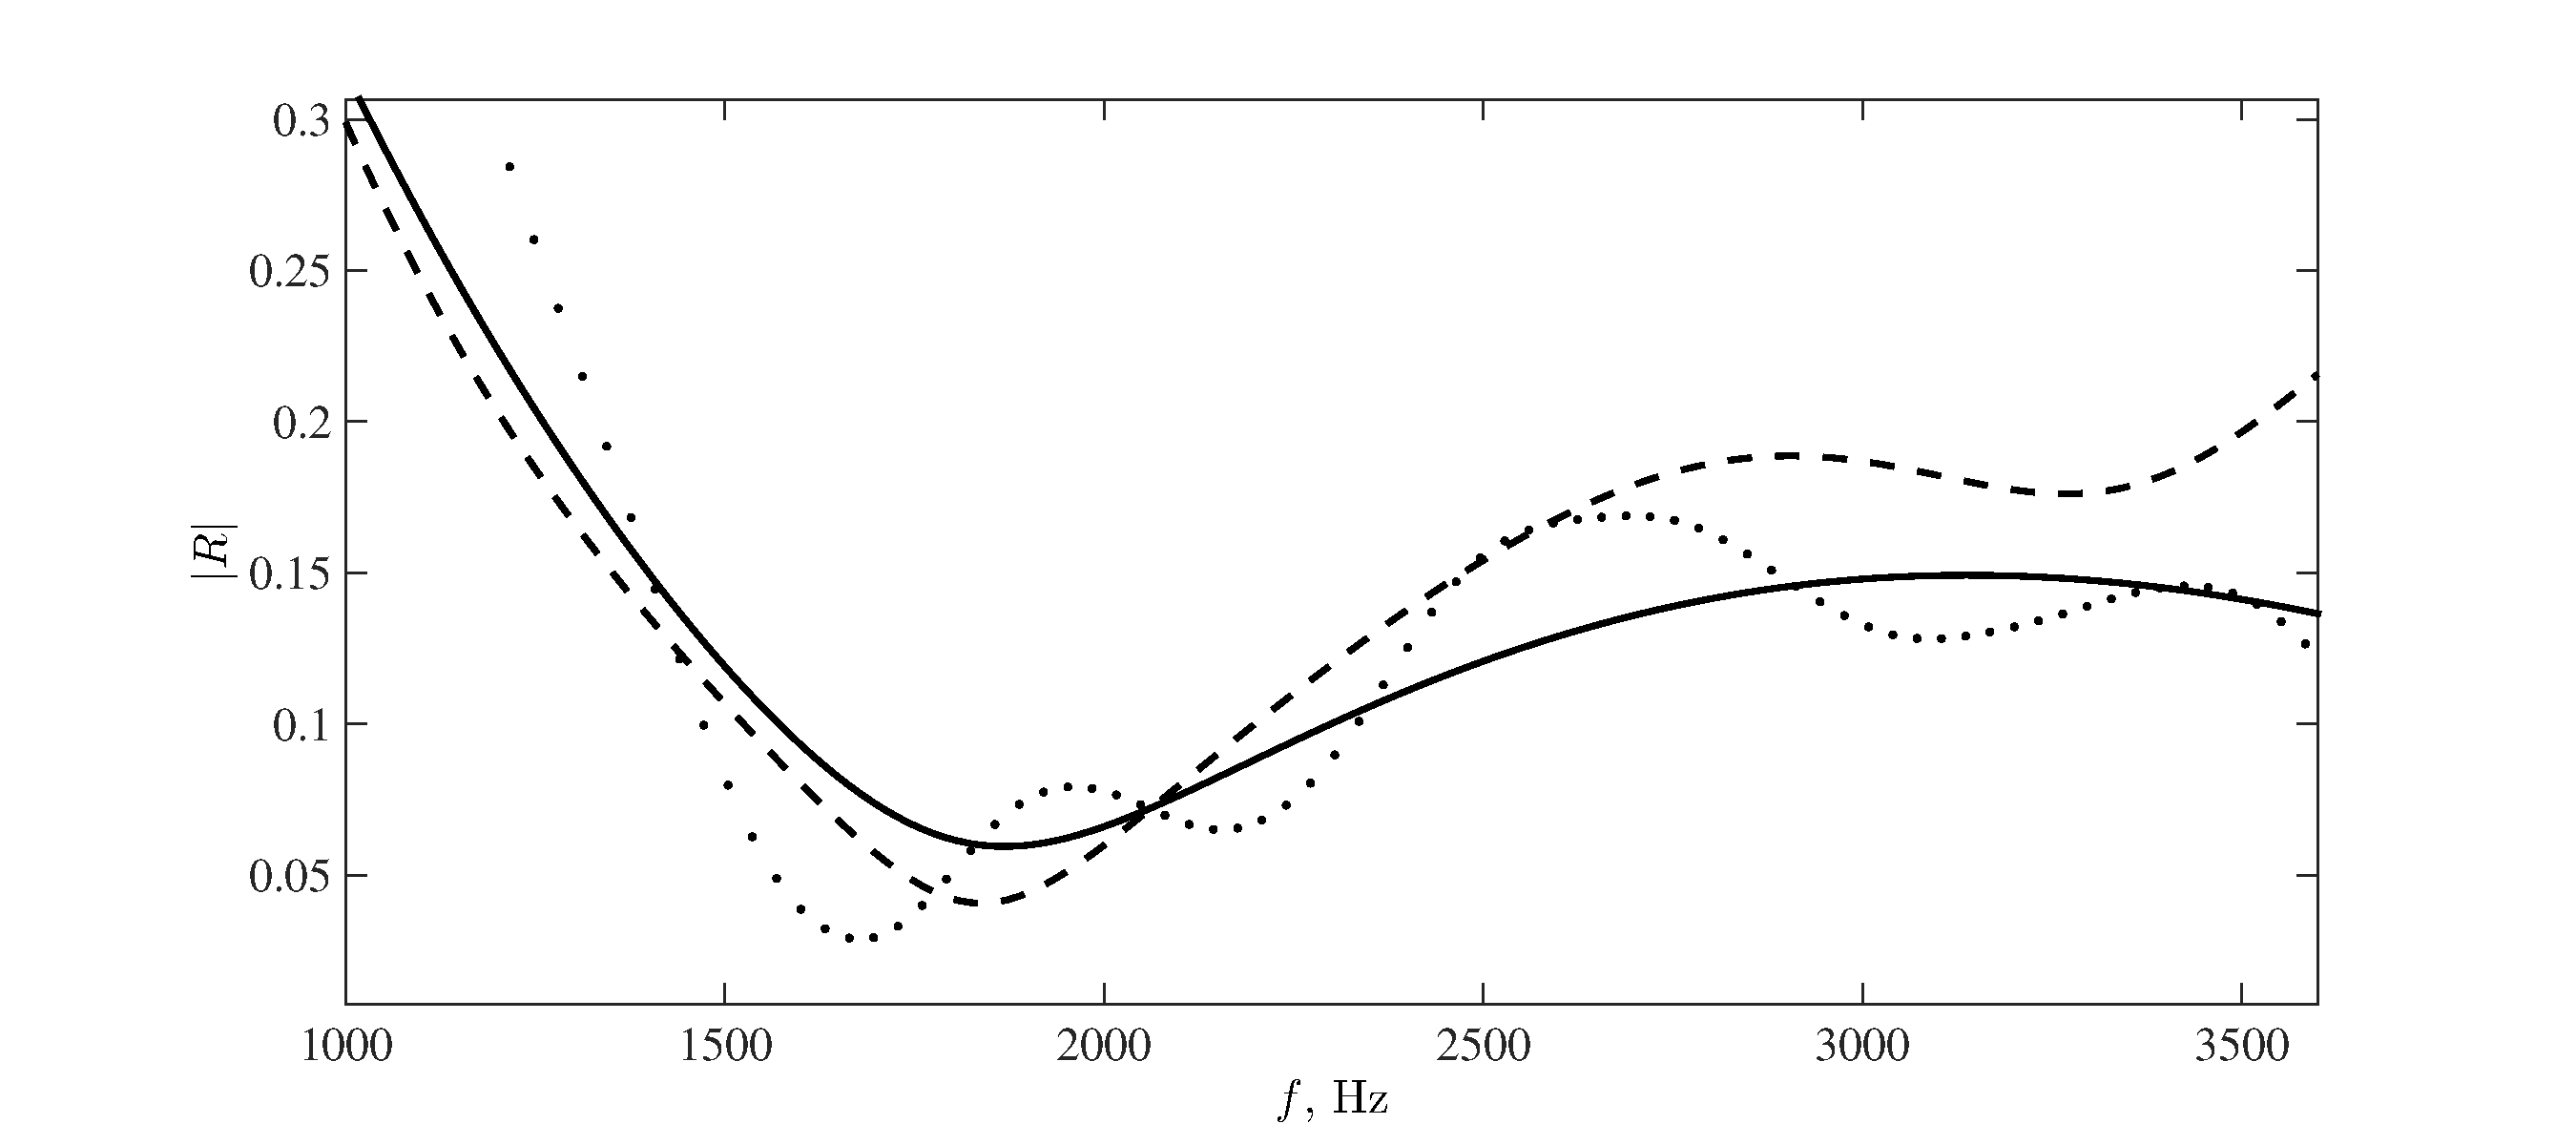
\includegraphics [scale=0.4] {ris1_6}
	\caption{График зависимости модуля коэффициента отражения $|R|$ при угле падения равном $30^\circ$. Пунктирной линией обозначен результат, полученный с помощью формулы ~\eqref{eq:reflectedfield2}, точками – с помощью формул ~\eqref{eq:reflectionsum}, ~\eqref{eq:mainequation}, сплошной линией – результат теоретического расчета на основе модели Био.}
\end{figure}

\begin{figure}[ht]
	\centering
	\label{img:ris1_7}
	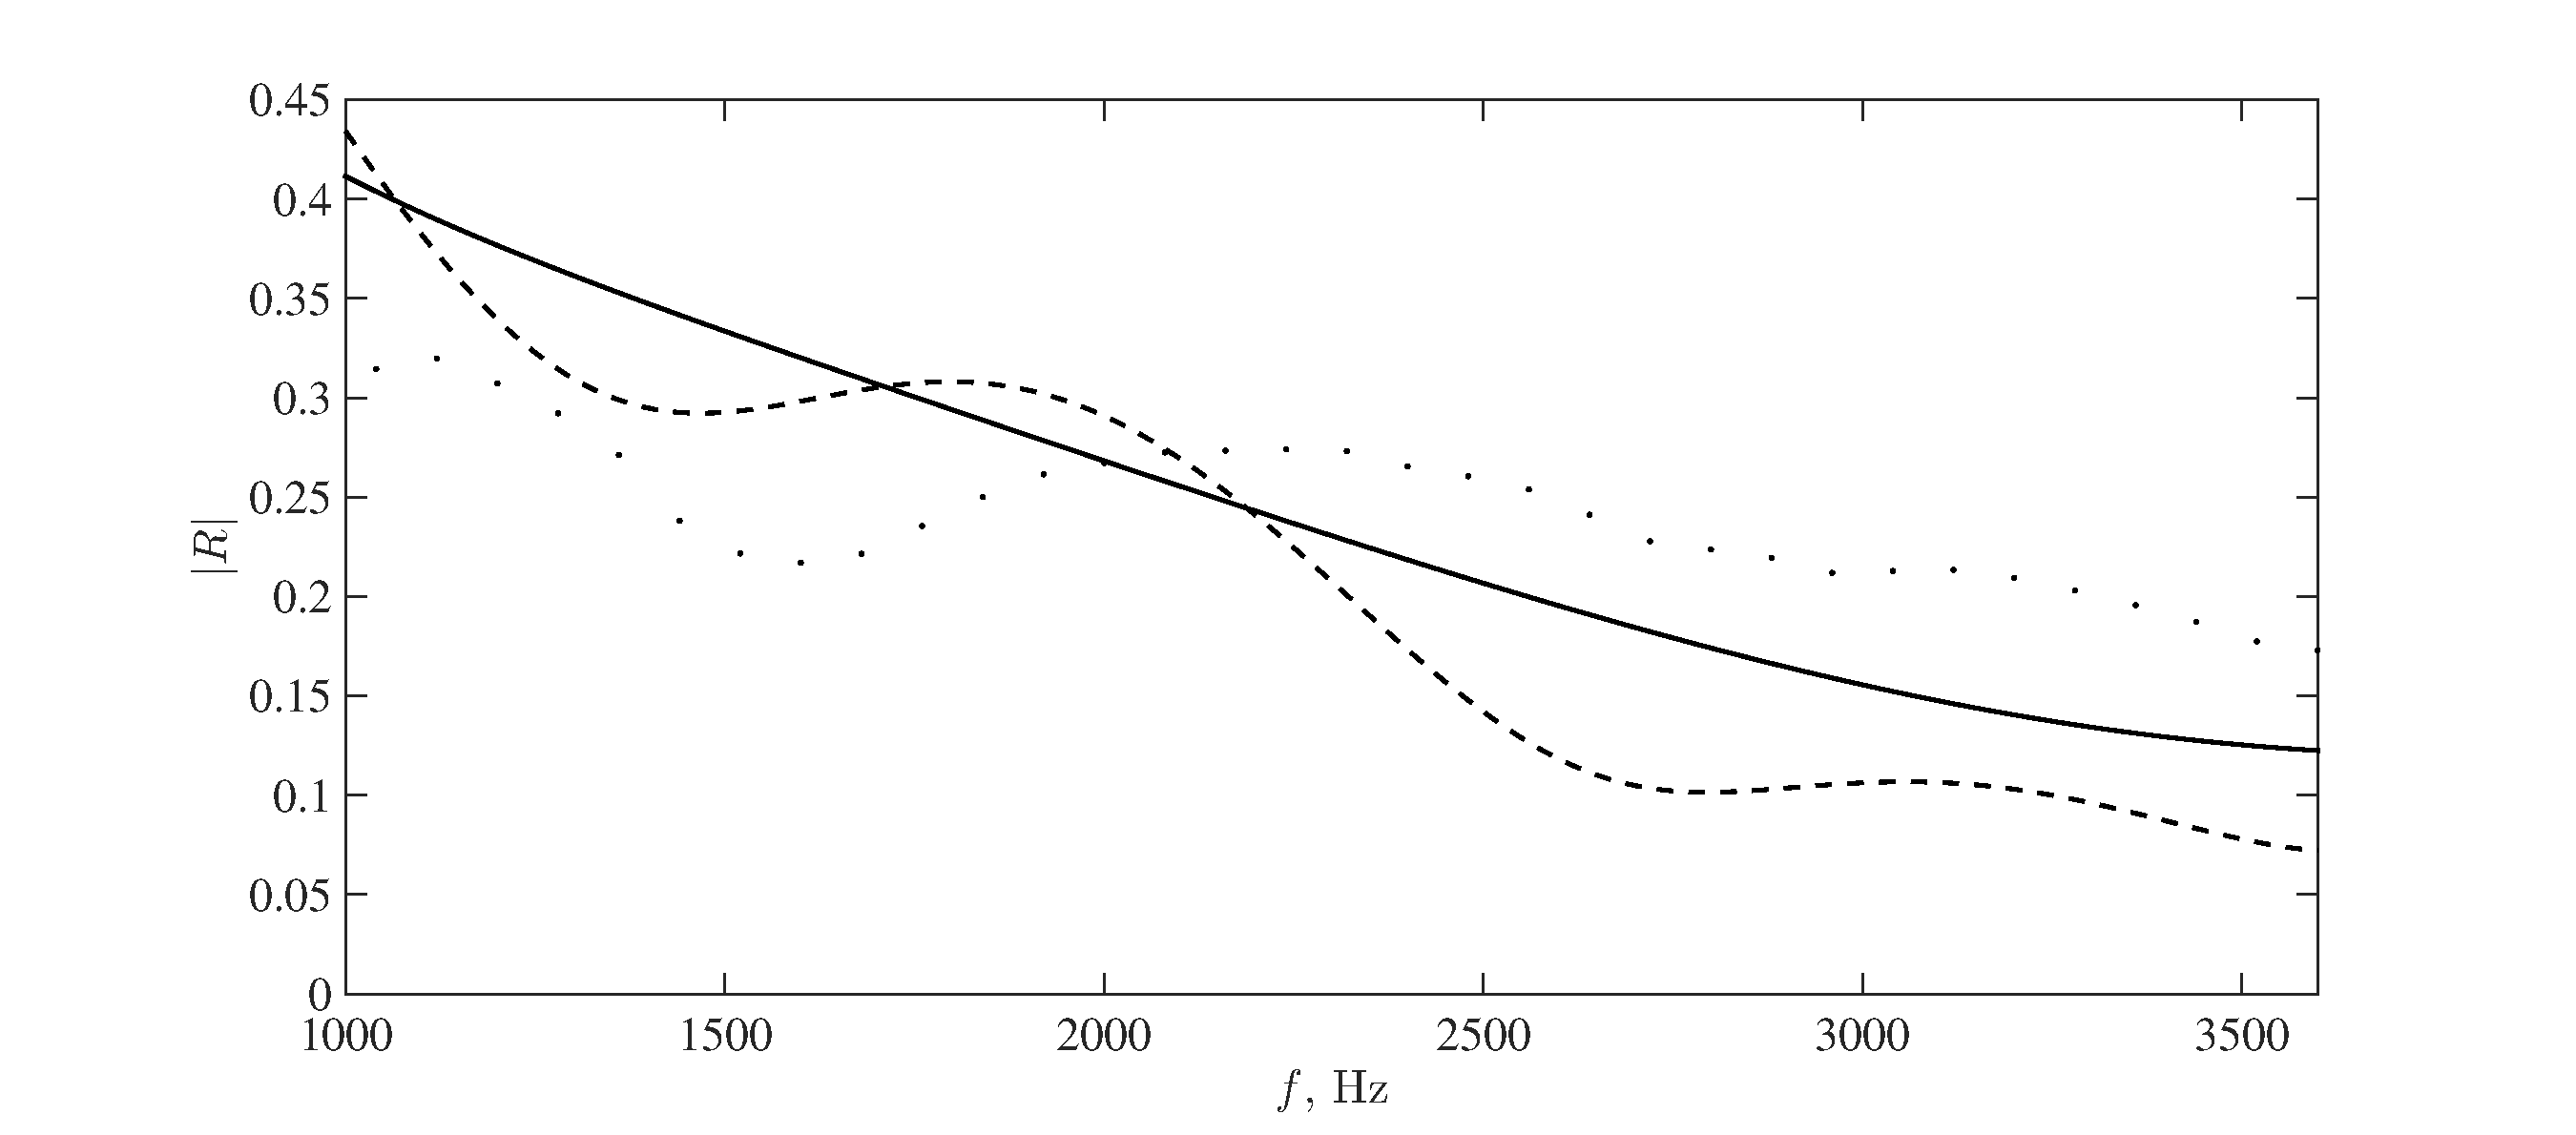
\includegraphics [scale=0.4] {ris1_7}
	\caption{График зависимости модуля коэффициента отражения $|R|$ при угле падения равном $60^\circ$. Пунктирной линией обозначен результат, полученный с помощью формулы ~\eqref{eq:reflectedfield2}, точками – с помощью формул ~\eqref{eq:reflectionsum}, ~\eqref{eq:mainequation}, сплошной линией – результат теоретического расчета на основе модели Био.}
\end{figure}

Результаты сравнения действительных частей коэффициентов отражения для нескольких частот представлены на Рис. ~\eqref{img:ris1_5}, ~\eqref{img:ris1_6}, ~\eqref{img:ris1_7}. Пунктирной линией обозначен результат, полученный с помощью формулы ~\eqref{eq:reflectedfield2}, точками – с помощью формул ~\eqref{eq:reflectionsum}, с кусочно-линейными интерполяционными функциями ~\eqref{eq:shapefunctions}, сплошной линией – результат теоретического расчета на основе модели Био \cite{Biot1956_I, Biot1956_II}. В качестве параметров модели Био использовались параметры, измеренные экспериментально в работе \cite{Geebelen2007} (см. таблицу).

\begin{table}
	\label{tabular:melamine}
	\begin{center}
		\begin{tabular}{cc}
			Пористость (\textit{англ.} porosity) [1] $\Phi$ & $0.99$ \\
			Сопротивление потоку (\textit{англ.} flow resistivity) $\sigma$ $[\text{Нм}^{-4} с]$ & $12000$ \\
			Термическая проницаемость (\textit{англ.} thermal permeability) $k'_0$ $[1]$ & $1.5 \times 10^{-9}$\\
			Масштаб вязкости (\textit{англ.} viscous dimension) $\Lambda$ $[\text{м}]$ & $100\times 10^{-6}$ \\	
			Тепловой масштаб (\textit{англ.} thermal dimension) $\Lambda'$ $[\text{м}]$ & $400\times 10^{-6}$\\
			Плотность материала $\rho_s$ $[\text{кг/м}^3]$ & $9$\\
			Сдвиговый модуль $N$ $[\text{кПа}]$ & $86(1 + 0.05i)$\\
			Коэффициент Пуассона $\nu$ & $0.276$
		\end{tabular}
	\end{center}
	\caption{Параметры пористого меламина.}
\end{table}

Как видно из Рис. ~\eqref{img:ris1_5}, ~\eqref{img:ris1_6}, ~\eqref{img:ris1_7}, при углах падения, для которых проводился эксперимент, описанная техника дает удовлетворительное соответствие с теорией Био и может быть использована для измерения угловых зависимостей коэффициентов отражения для имеющихся и новых звукопоглощающих материалов. Некоторое несоответствие экспериментальных и теоретических результатов авторы объясняют внутренними шумами экспериментальной установки, ошибками в измерении геометрии эксперимента и тем, что образец исследуемого материала был собран из различных прямоугольных кусков, слегка отличающихся по форме и свойствам.
           % Глава про меламин
\chapter{Измерение импульсного отклика акустического MLS-сигнала в среде с потоком}

\section{Введение}
В данное время широко используемым методом измерения импульсных откликов и частотных характеристик различных акустических рассеивателей является техника измерения импульсного отклика с помощью псевдослучайной последовательности максимальной длины (Maximum Length Sequence) \cite{ValyaevMLS, ValyaevRoad, Denisov2017}. Суть техники заключается в зондировании испытуемой системы квазишумовой посылкой, автокорреляционная функция которой близка к дельта-функции, и последующей корреляционной обработке полученных данных.

Ценность дифракционного MLS-эксперимента состоит в возможности непосредственного наблюдения полей, дифрагированных на различных, в том числе и сложных, объектах. В данной работе ставится практически важная задача применить технику MLS-эксперимента в случае прохождения акустического сигнала через воздушную струю.

Эксперименты по изучению воздушных струй акустическими методами уже проводились и описаны в существующих работах. В \cite{Candel1976} изучается экранирование струей монохроматического сигнала в зависимости от взаимных ориентаций струи и источника сигнала. Аналитическая модель этого процесса предложена в \cite{Gerhold1983}. Вопрос о поведении фазы акустической волны при прохождении через турбулентный поток численно рассмотрен в \cite{Karweit1991}. Экспериментальное изучение случайных характеристик струи на основе поведения монохроматической акустической волны, проходящей через струю перпендикулярно направлению потока, проведено в \cite{HoChi}.
 
Имеются и работы по изучению влияния акустических волн на потоки воздуха с небольшими скоростями \cite{Golovanov2006, Vlasov1971}. В данной работе такое влияние не рассматривается.

Кроме того, имеется множество работ, посвященных отражению и прохождению акустических волн через тангенциальный разрыв на плоской границе двух движущихся жидкостей \cite{Friedland1969, Godin1988, Jones1973, Gottlieb1960}. 

В \cite{Ahuja1981} описаны эксперименты по корреляционному детектированию широкополосного сигнала, проходящего через воздушную струю. В первом из них точечный источник помещался на оси потока, рядом с ним располагался контрольный микрофон, а снаружи потока размещался измерительный микрофон. По корреляции между сигналами с микрофонов определялась задержка прохождения сигнала и, соответственно, угол рефракции на границе потока. Во втором эксперименте источник с контрольным микрофоном также находится на оси потока, а два измерительных располагаются вне потока и на оси потока ниже по течению. Рассматривая поток, как отличную от воздуха среду, авторы измеряют и моделируют углы преломления и отражения на границе поток-пространство. 

В данной работе с помощью монопольного источника и MLS-техники \cite{ValyaevMLS, ValyaevRoad, Denisov2017} производится экспериментальное измерение импульсного отклика при наличии потока на акустической трассе. Изучаются явления сноса сигнала потоком и фокусировки сигнала цилиндрической струей. Проводится математическое моделирование этого процесса путем решения уравнения для распространения звука в постоянном потоке \cite{Blokhitsev1981} методом конечных разностей.

\section{Описание эксперимента}
Эксперименты проводились в заглушенной камере с потоком АК-2 ЦАГИ. Схема эксперимента показана на (Рис. \ref{img:ris2_1}). На рисунке показана система координат $(x,y,z)$, используемая ниже для задания положений микрофонов и источника.

Поток воздуха со скоростями $20, 40, 60, 80$ м/с создавался соплом круглого сечения диаметром $40$ см. На некотором расстоянии от сопла были расположены $3$ микрофона и источник звука, так чтобы акустическая трасса проходила через струю (Рис. \ref{img:ris2_1}). Была проведена серия экспериментов, в которых акустическая трасса была как перпендикулярна (Рис. \ref{img:ris2_2}), так и неперпендикулярна оси потока (Рис. \ref{img:ris2_3}).

\begin{figure}[ht]
	\centering
	\includegraphics [scale=1] {ris2_1}
	\caption{Схема эксперимента с потоком.}
	\label{img:ris2_1}
\end{figure}

\begin{figure}[ht]
	\centering
	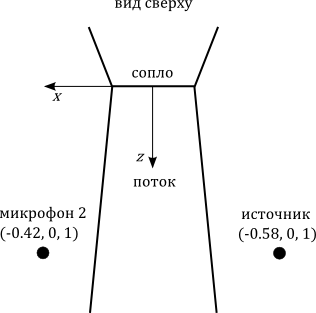
\includegraphics [scale=1] {ris2_2}
	\caption{Геометрия эксперимента. Акустическая трасса перпендикуляра оси потока.}
	\label{img:ris2_2}
\end{figure}

\begin{figure}[ht]
	\centering
	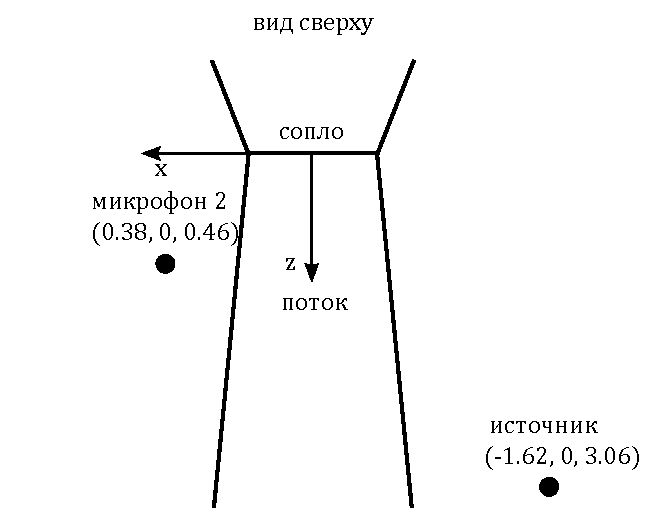
\includegraphics [scale=1] {ris2_3}
	\caption{Геометрия эксперимента. Акустическая трасса неперпендикулярна оси потока.}
	\label{img:ris2_3}
\end{figure}

Экспериментальное оборудование и алгоритм корреляционной обработки данных были аналогичны таковым, описанным в \cite{ValyaevMLS, ValyaevRoad, Denisov2017}. В качестве источника использовался всенаправленный излучатель Omnisource тип 4295 фирмы Bruel \& Kjaer с датчиком объемной скорости, в качестве микрофонов применялись ¼-дюймовые микрофоны типа 4935 фирмы Bruel \& Kjaer.

\section{Теоретическое описание}
Полноценное описание волновых процессов в среде с потоком было дано в \cite{Blokhitsev1981}. В данной монографии указывается, что скорость потока может быть представлена в виде средней скорости и флуктуации. Средняя скорость обуславливает снос и фокусировку звуковой волны, а переменная часть скорости ведет к рассеянию звука на флюктуациях. Для описания эффектов, связанных с переменной составляющей потока, необходимы данные о масштабах флуктуаций его скорости. Измерения этих масштабов в настоящей работе не производились. Ниже будет дано теоретическое описание эффектов, обусловленных постоянной составляющей потока.

\subsection{Расчет сноса звукового поля}
Для оценки сноса акустического сигнала будем рассматривать упрощенную двумерную (в координатах $x, z$ ) модель (Рис. \ref{img:ris2_4}). Будем считать, что скорость потока постоянна внутри струи и равна нулю за её пределами. Тогда, акустический потенциал $\Phi$  удовлетворяет уравнению \cite{Blokhitsev1981}:

\begin{equation}
\label{eq:2_1}
\left(\frac{\partial^2}{\partial x^2} + \frac{\partial^2}{\partial z^2}\right) \Phi = \left(M \frac{\partial}{\partial z} + \frac{1}{c} \frac{\partial}{\partial t}\right)^2 \Phi,
\end{equation}
где $M = V/c$ – число Маха, а $V$ – скорость потока. Здесь подразумевается, что $M$ постоянно внутри потока и равно нулю снаружи. Для корректной постановки задачи накладываются условия непрерывности давления и нормальной компоненты скорости на границе.
Используя принцип локальности \cite{Keller1962}, выпишем представление акустического потенциала звукового поля на приемнике в виде фазового интеграла, полученного в \cite{Mironov1975}: 

\begin{equation}
\label{eq:2_2}
\Phi = \int \int A(\omega) \exp(i f (\omega, k_z)) d\omega dk_z,
\end{equation}

\begin{equation}
\label{eq:2_3}
f(\omega, k_z) = -\omega t + k_z(z_2 - z_1) + (x_2 - x_1 - H) \sqrt{\frac{\omega^2}{c^2} - k_z^2} + H\sqrt{\left(\frac{\omega}{c} - Mk_z\right)^2 - k_z^2}
\end{equation}

Этот интеграл получен в результате применения преобразования Фурье к уравнению ~\eqref{eq:2_1} по времени и по координате $z$, направленной вдоль потока. В функции $f$ ~\eqref{eq:2_3} третий член описывает распространение вдоль оси $x$ в пространстве без потока, а четвертый член описывает распространение в пространстве с потоком. 

\begin{figure}[ht]
	\centering
	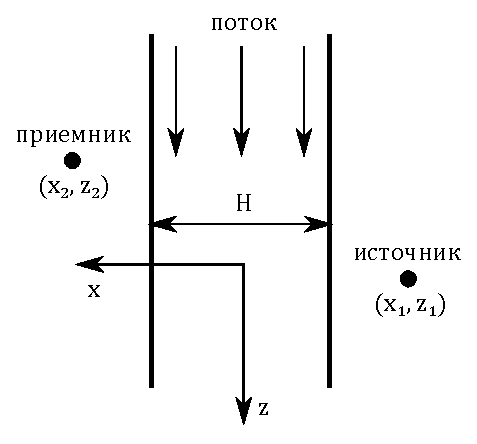
\includegraphics [scale=1] {ris2_4}
	\caption{Двухмерная модель.}
	\label{img:ris2_4}
\end{figure}

В случаях, когда длины волн меньше характерных масштабов неоднородностей, для анализа фазовых интегралов обычно применяют метод стационарной фазы или метод перевала \cite{SveshnikovTFKP}. В рассматриваемом случае интеграла ~\eqref{eq:2_2} необходимо применять метод стационарной фазы для двух комплексных переменных, для чего в комплексной плоскости переменных $(\omega, k_z)$ необходимо отыскать стационарные точки, в которых для подынтегральной функции выполняются условия.

\begin{equation}
\label{eq:2_4}
\frac{\partial f}{\partial \omega} = 0, \quad \frac{\partial f}{\partial k_z} = 0.
\end{equation}

В окрестностях стационарных точек осцилляции подынтегральной функции замедляются, и поэтому эти точки дают существенный вклад в интеграл, а в окрестности остальных точек подынтегральная функция быстро осциллирует, и поэтому такие окрестности не дают существенного вклада в интеграл.

Введем переменную $\gamma = k_z/(\omega/c)$  и перепишем ~\eqref{eq:2_3} в виде:

\begin{equation}
\label{eq:2_5}
f(\omega, \gamma) = \omega \left[-t + \frac{\gamma(z_2 - z_1)}{c} + \frac{x_2 - x_1 - H}{c} \sqrt{1 - \gamma^2} + \frac{H}{c} \sqrt{(1 - M\gamma)^2 - \gamma^2}\right]
\end{equation}

Условия ~\eqref{eq:2_4} перепишутся как 

\begin{equation}
\label{eq:2_6}
\frac{\partial f}{\partial \omega} = 0, \quad \frac{\partial f}{\partial \gamma} = 0,
\end{equation}
т.е.
\begin{equation}
\label{eq:2_7}
t = \frac{\gamma_* (z_2 - z_1)}{c} + \frac{x_2 - x_1 - H}{c} \sqrt{1 - \gamma_*^2} + \frac{H}{z} \sqrt{(1 - M\gamma_*)^2 - \gamma_*^2}
\end{equation}
где $\gamma_*$ - корень уравнения 
\begin{equation}
\label{eq:2_8}
(z_2 - z_1) - (x_2 - x_1 - H) \frac{\gamma}{\sqrt{1 - \gamma^2}} - H \frac{\gamma + M(1 - M \gamma)}{\sqrt{(1 - M\gamma)^2 - \gamma^2}} = 0.
\end{equation}

Решения уравнений ~\eqref{eq:2_7} и ~\eqref{eq:2_8} дают оценку времени прихода сигнала.

В общем случае время прихода сигнала $t$ для случая с потоком будет отличаться от времени распространения сигнала при отсутствии потока. Причина этого физически очевидна – часть времени сигнал распространяется против потока, что уменьшает фазовую скорость сигнала. В случае распространения звука по потоку время прохождения сигнала уменьшится. В данной работе случай ускорения звука не рассматривается, и соответствующий эксперимент проведен не был. 

\subsection{Расчет фокусировки звукового поля}

Если проекция единичного вектора вдоль звукового луча на скорость потока отрицательна, то фазовая скорость сигнала, распространяющегося вдоль такого луча, уменьшается, и, тем самым, поток может рассматриваться как акустически менее плотная среда.  В этом случае цилиндрический поток выступает как собирающая линза. Схема фокусировки показана на (Рис. \ref{img:ris2_6}).

\begin{figure}[ht]
	\centering
	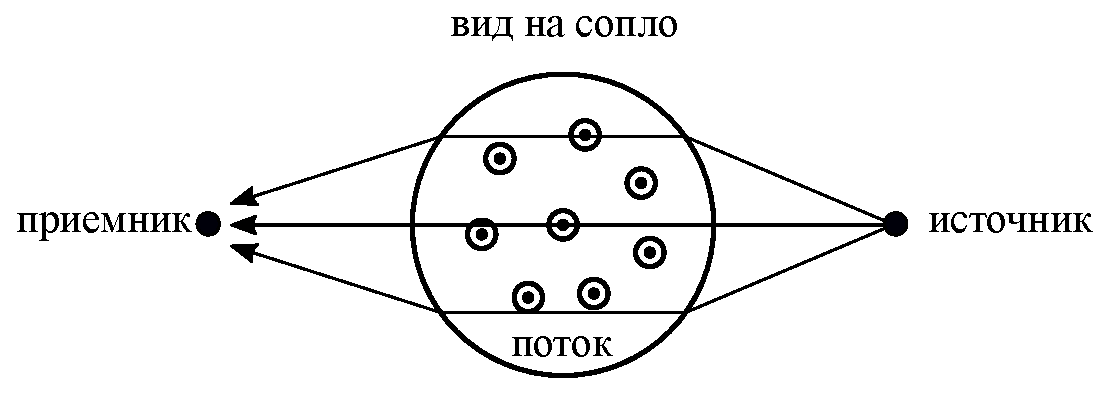
\includegraphics [scale=0.7] {ris2_6}
	\caption{Фокусировка звука потоком}
	\label{img:ris2_6}
\end{figure}

Для расчета эффекта фокусировки необходимо рассматривать трехмерную модель. Таким образом, следует решать уравнение:
\begin{equation}
\label{eq:2_9}
\left(\frac{\partial^2}{\partial x^2} + \frac{\partial^2}{\partial y^2} + \frac{\partial^2}{\partial z^2}\right)\Phi = \left(M + \frac{\partial}{\partial z} + \frac{1}{c} \frac{\partial }{\partial t}\right) ^2 \Phi,
\end{equation}
где $M$ отлично от нуля внутри потока, и равно нулю снаружи. Как и ранее, предполагается, что на границе потока выполнены стандартные условия непрерывности.

В простейшем случае можно предположить, что поток имеет цилиндрическую форму и число Маха в любой его точке постоянно. Однако такое представление не описывает реальной физической картины уже на расстояниях порядка одного калибра от сопла. Ниже предлагается более ''реалистичная'' форма потока.

Как известно, поток состоит из начального участка, переходного и основного участков \cite{Abramovitz}. Для простоты будем полагать, что длина переходного участка равна нулю. В начальном участке струя имеет потенциальное ядро течения конусовидной формы. Скорость в этом ядре постоянна. Убывание скорости вне ядра может быть описано следующим Гауссовым законом \cite{Tam}:

\begin{equation}
\label{eq:2_10}
V =
\begin{cases}
V_0, (r<h) \\
V_0 \exp\left(-\ln 2 \left[\frac{r - h(z)}{b(z)}\right]^2\right), \quad (r \geq h).
\end{cases}
\end{equation}

Здесь $h(z)$ – радиус ядра, $b(z)$ – полуширина слоя смешения, $r = \sqrt{x^2 + y^2}$, $V_0$ – скорость потока в ядре. Аналогичным образом скорость потока может быть рассчитана и на основном участке:

\begin{equation}
\label{eq:2_11}
V = V_c\left[- \ln 2 \left(\frac{r}{b(z)}\right)^2\right],
\end{equation}
где $V_c$ – скорость на оси потока. Мы предполагаем, что скорость на оси потока спадает обратно пропорционально расстоянию от сопла. Здесь $b(z)$ – расстояние от оси ядра до окружности, на которой скорость ядра спадает вдвое. Параметры $h(z), b(z)$ оценивались на основе данных анемометрии для сопла диаметром $0.6$ м, на скоростях $50, 45$ и $35$ м/с. Пример экспериментальных данных для начального участка струи и расчета по формуле ~\eqref{eq:2_10} приведен на (Рис. \ref{img:ris2_7}).

\begin{figure}[ht]
	\centering
	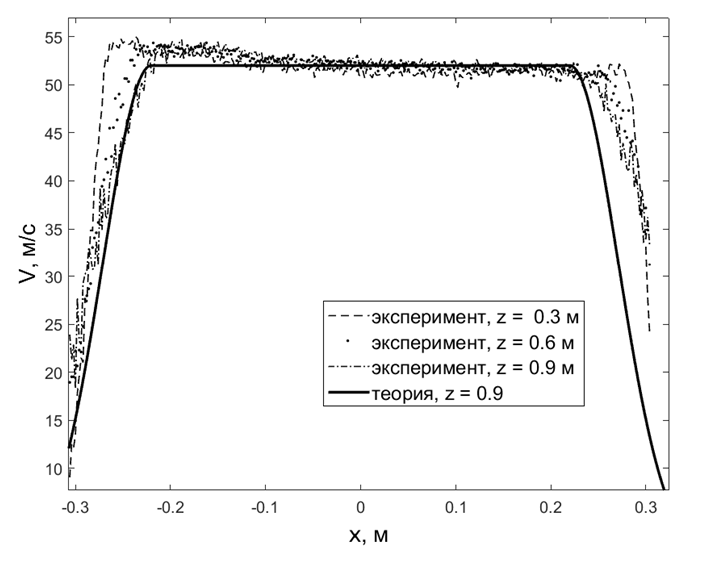
\includegraphics [scale=0.8] {ris2_7}
	\caption{Данные термоанемометрии потока для скорости 55 м/c и сравнение с теоретическим расчетом по формуле ~\eqref{eq:2_10}.}
	\label{img:ris2_7}
\end{figure}

В общем случае для потенциального неоднородного потока решается уравнение Блохинцева, а для неоднородного потока с завихрениями – уравнение Блохинцева-Хоу \cite{Munin1981}, стр. 22. В данной работе рассматриваемый поток неоднороден и завихрен в слое смешения, однако при малых числах Маха уравнение Блохинцева-Хоу переходит в уравнение ~\eqref{eq:2_1}. Поэтому для расчета амплитуды сфокусированного сигнала численно решалось уравнение ~\eqref{eq:2_1} с помощью метода конечных разностей. Производные по пространственным координатам заменялись симметричными конечно-разностными аппроксимациями первого порядка, интегрирование по времени осуществлялось с помощью метода Рунге-Кутта 4 порядка. Для подавления волн, отраженных от границ сетки использовался метод полностью согласованного слоя (PML) \cite{Grothe2010}. Шаг сетки выбирался равным $2$ см. Такой выбор позволил корректно описывать распространение волн в частотном диапазоне до $2$ кГц.

\section{Экспериментальные результаты и моделирование}
Сигналы, полученные в эксперименте, подвергались корреляционной обработке, алгоритм которой подробно изложен в \cite{ValyaevMLS, ValyaevRoad, Denisov2017}. Коротко говоря, в обработку входит вычисление корреляции с эталонным MLS-сигналом, вычисление объемной скорости источника по методу двух микрофонов и фильтрация в частотной области. В результате получается импульсный отклик акустического тракта. Нормировка амплитуды для простоты выбирается таким образом, чтобы максимальное значение сигнала было равно единице на расстоянии $1$ м от источника. Сигналы подвергаются полосовой фильтрации в диапазоне $500-4000$ Гц. 

Результаты корреляционной обработки сигнала на микрофоне 2 для случая перпендикулярной и неперпендикулярной трасс распространения представлены на (Рис. \ref{img:ris2_8} и \ref{img:ris2_8} соответственно).

\begin{figure}[ht]
	\centering
	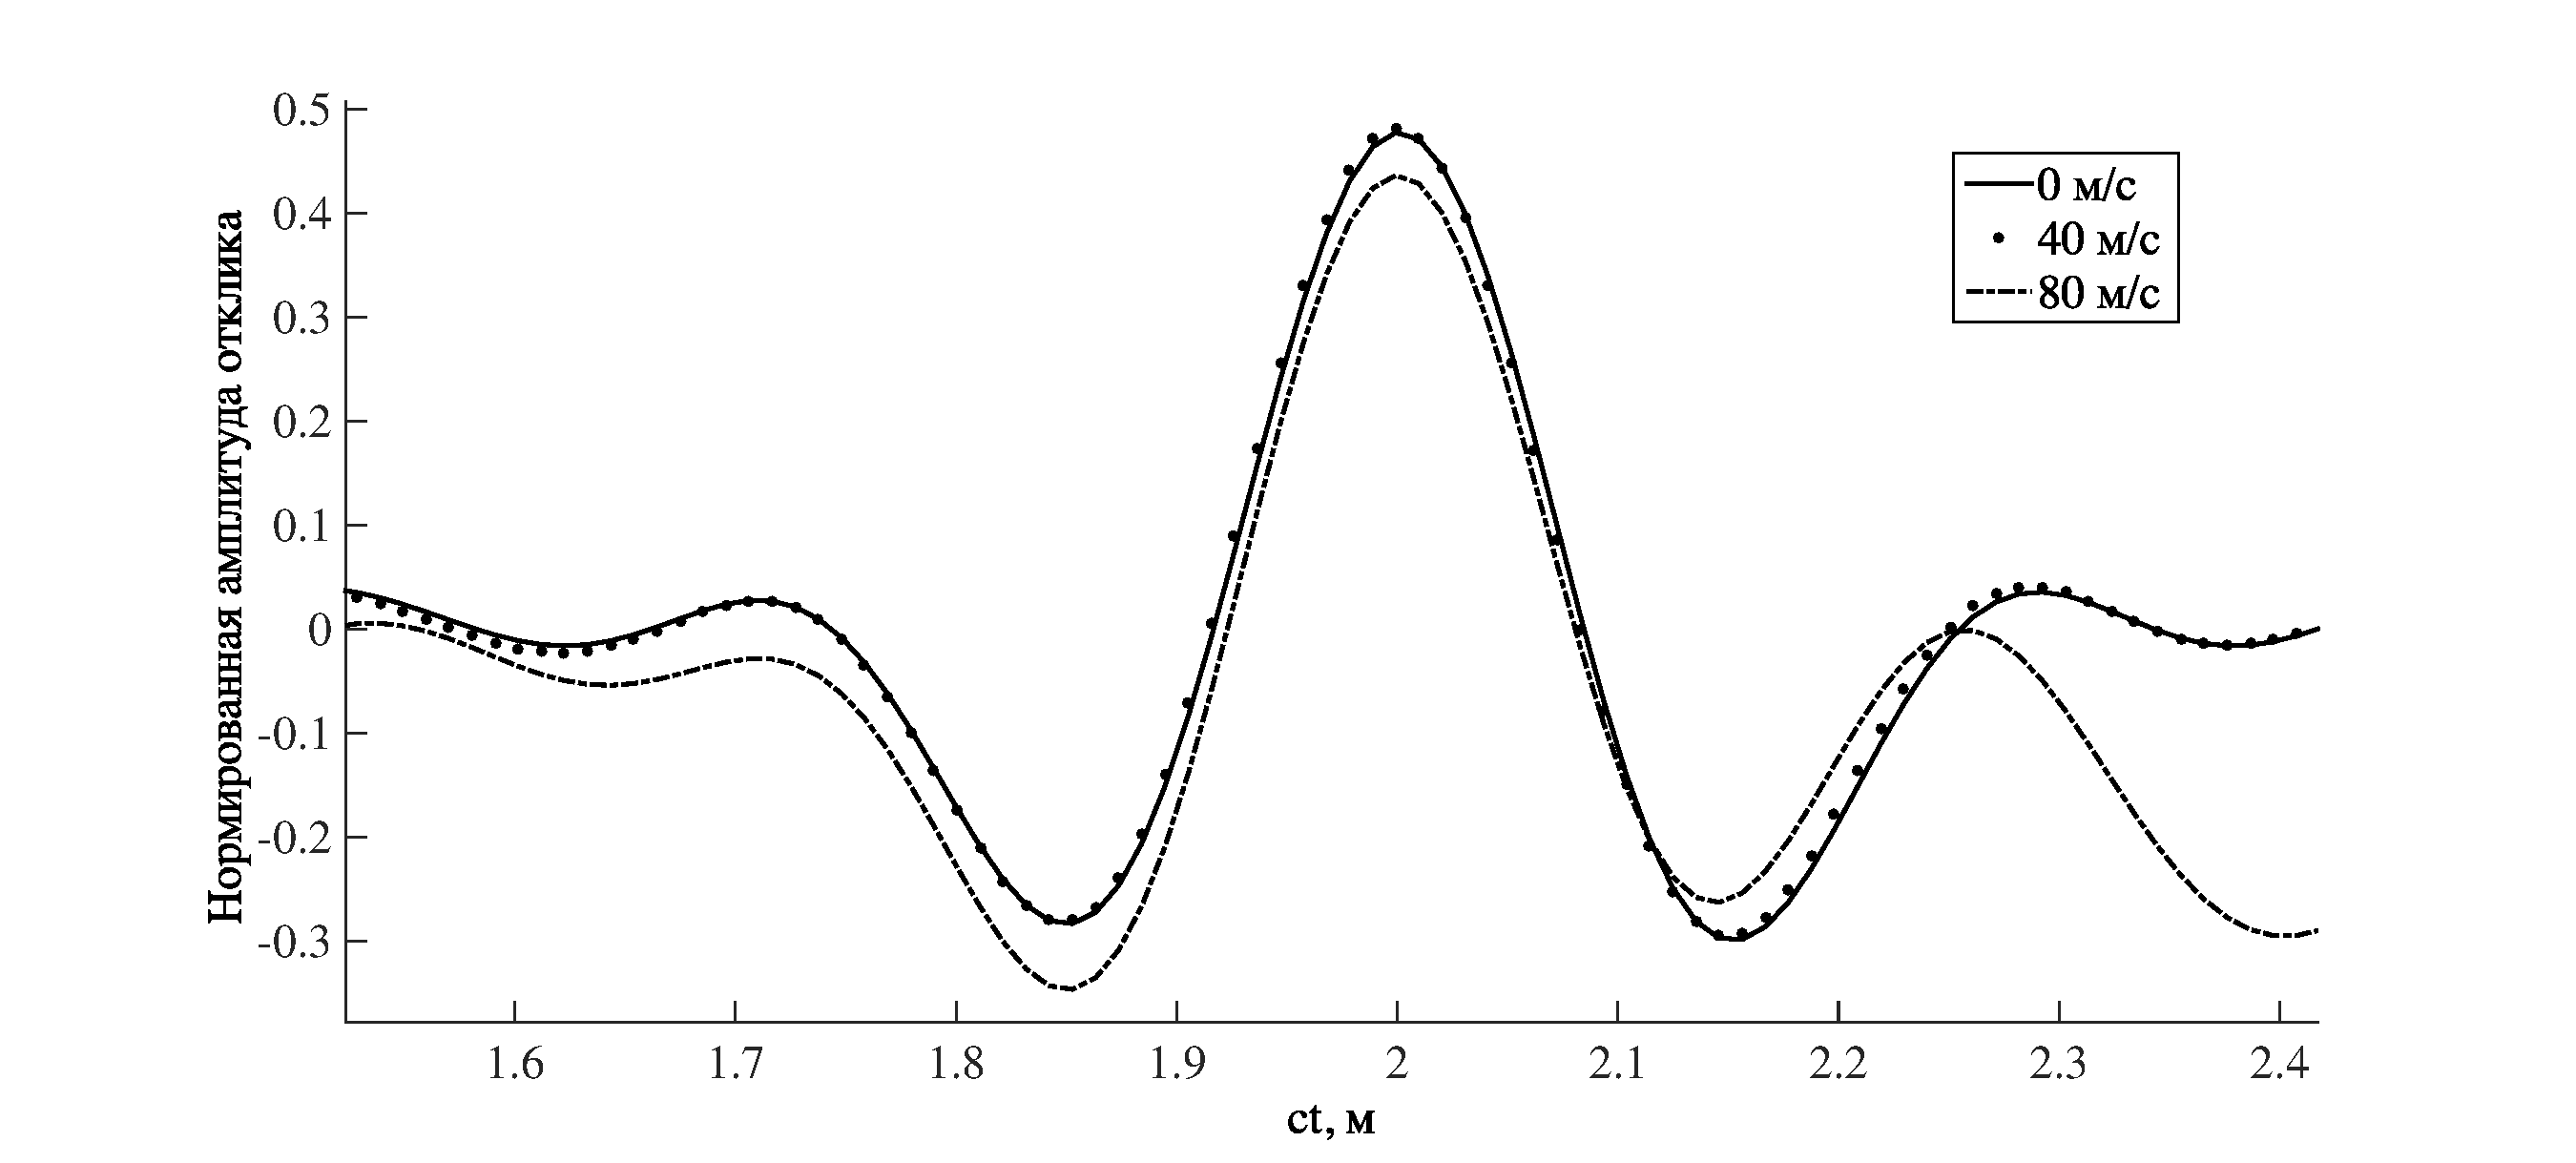
\includegraphics [scale=0.4] {ris2_8}
	\caption{Отклики на микрофоне 2 в случае, когда акустическая трасса перпендикулярна оси потока.}
	\label{img:ris2_8}
\end{figure}

\begin{figure}[ht]
	\centering
	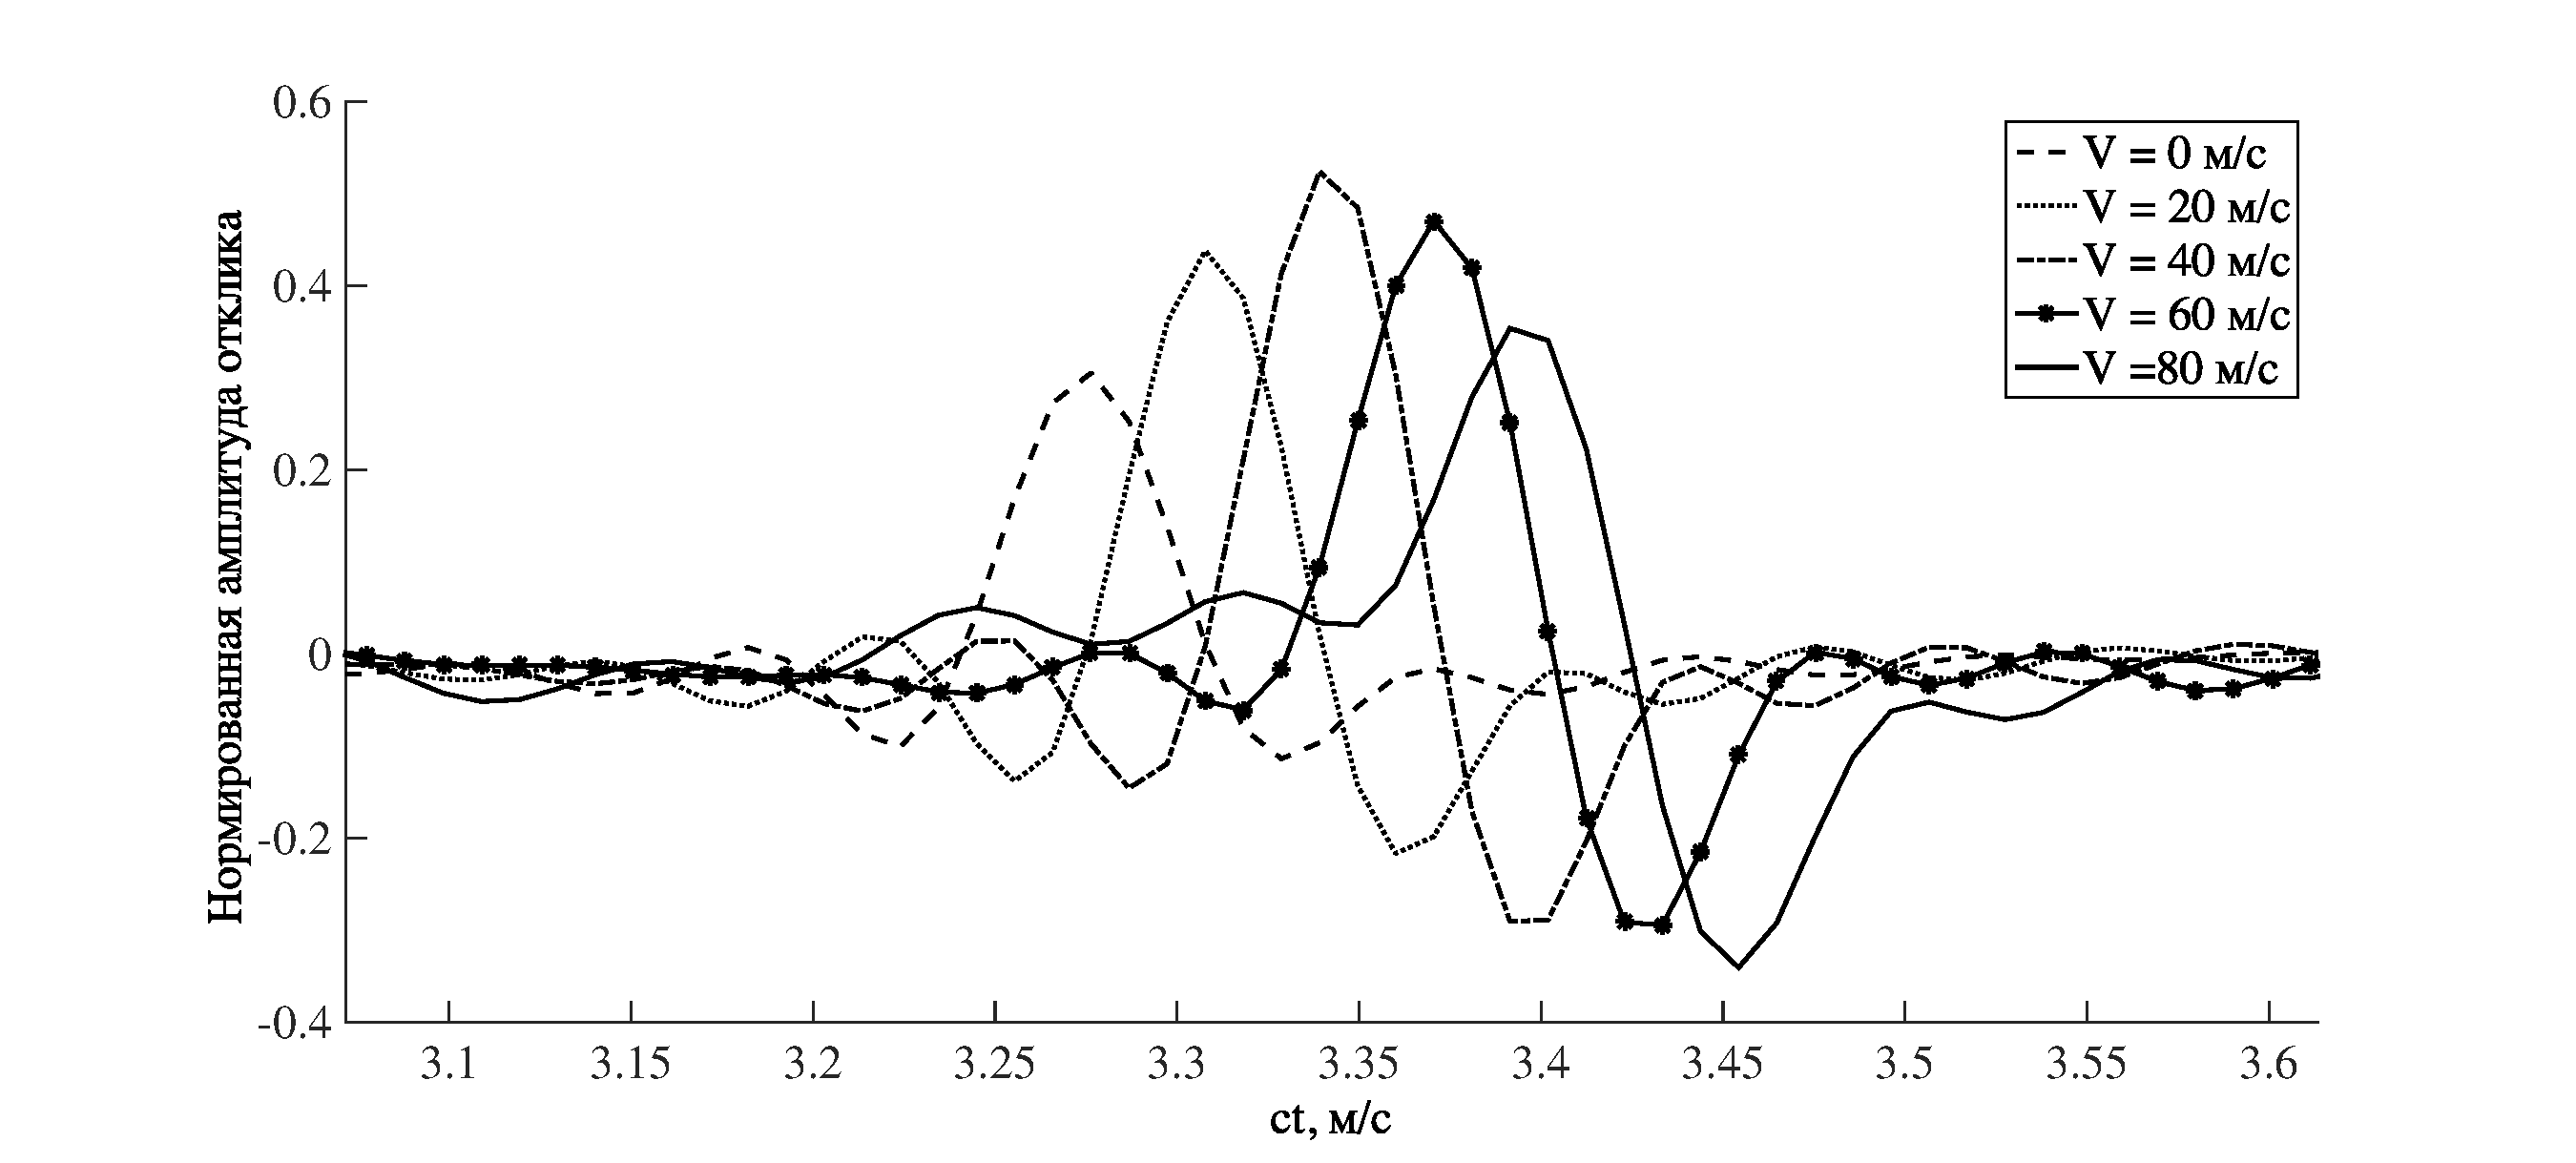
\includegraphics [scale=0.4] {ris2_9}
	\caption{Отклики на микрофоне 2 в случае, когда акустическая трасса неперпендикулярна оси потока.}
	\label{img:ris2_9}
\end{figure}


Из представленных результатов следует, что влияние потока в случае перпендикулярной трассы распространения незначительно. Отсутствие сноса сигнала и фокусировки объясняется тем фактом, что проекция луча на поток ($z$-компонента волнового вектора) в данном случае равна нулю. В случае неперпендикулярной трассы распространения, увеличение средней скорости потока приводит к увеличению задержки сигнала. Кроме того, для потоков $0, 20$ и $40$ м/c наблюдается рост амплитуды с ростом скорости потока. Наиболее вероятная причина этого роста – фокусировка сигнала. Также наблюдается падение амплитуды на скоростях $60$ м/с и $80$ м/с.

Моделирование уравнений ~\eqref{eq:2_7}, ~\eqref{eq:2_8} для координат микрофона 2 для случая неперпендикулярной трассы распространения, дает следующие значения времени задержки ~\eqref{tabular:zaderzhki}. Данные оценки неплохо согласуются с экспериментом.


\begin{table}
	\label{tabular:zaderzhki}
	\begin{center}
		\begin{tabular}{|l|l|l|l|l|l|}
			\hline
			 Поток        & Расчет         & Эксперимент    \\ \hline
			 $V = 0$  м/с & $ct = 3.280$ м & $ct = 3.280$ м \\ \hline
			 $V = 20$ м/с & $ct = 3.310$ м & $ct = 3.312$ м \\ \hline
			 $V = 40$ м/с & $ct = 3.339$ м & $ct = 3.343$ м \\ \hline			
			 $V = 60$ м/с & $ct = 3.366$ м & $ct = 3.375$ м \\ \hline			
			 $V = 80$ м/с & $ct = 3.394$ м & $ct = 3.395$ м \\ \hline
		\end{tabular}
	\end{center}
	\caption{Задержки сигналов, вычисленные с помощью ~\eqref{eq:2_7}, ~\eqref{eq:2_8} в сравнении с результатами эксперимента}
\end{table}	

На (Рис. \ref{img:ris2_10}) приводятся результаты численного моделирования сигналов методом конечных разностей для потока, скорость  струи в котором рассчитывалась с помощью ~\eqref{eq:2_10} и ~\eqref{eq:2_11}. Отметим, что результаты численного моделирования фильтруются в диапазоне $500-2000$ Гц в соответствии с пространственным разрешением сетки.

\begin{figure}[ht]
	\centering
	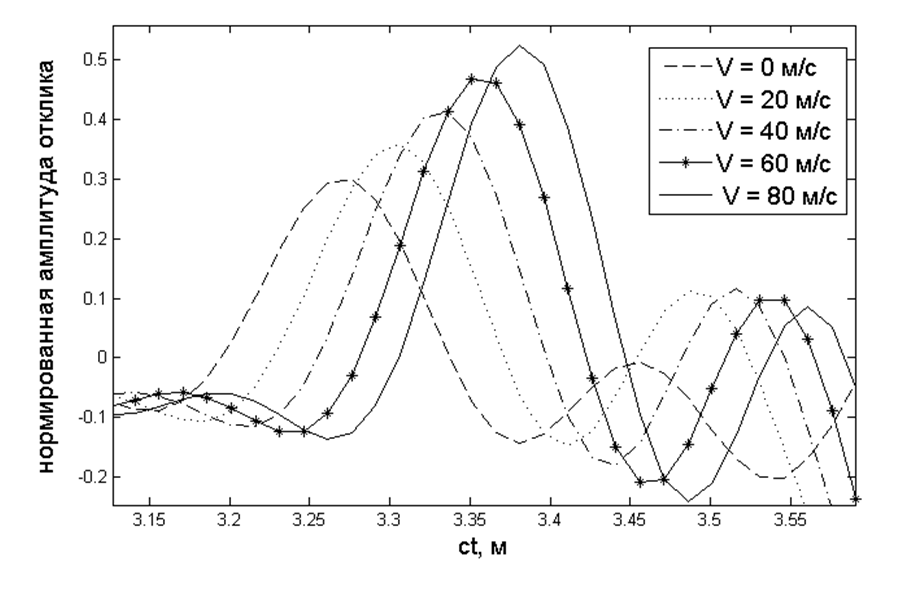
\includegraphics [scale=0.7] {ris2_10}
	\caption{Результат моделирования сигнала на микрофоне 2.}
	\label{img:ris2_10}
\end{figure}


Для наглядности на Рис. \ref{img:ris2_11}, Рис. \ref{img:ris2_12} совместно приведены результаты  численного моделирования и эксперимента для скоростей потока $20$ и $60$ м/с. Кроме струи ''реалистичной формы'', скорость которой рассчитывалась по формулам ~\eqref{eq:2_10} и ~\eqref{eq:2_11}, также представлены результаты моделирования для потока цилиндрической формы с постоянной по сечению скоростью.

\begin{figure}[ht]
	\centering
	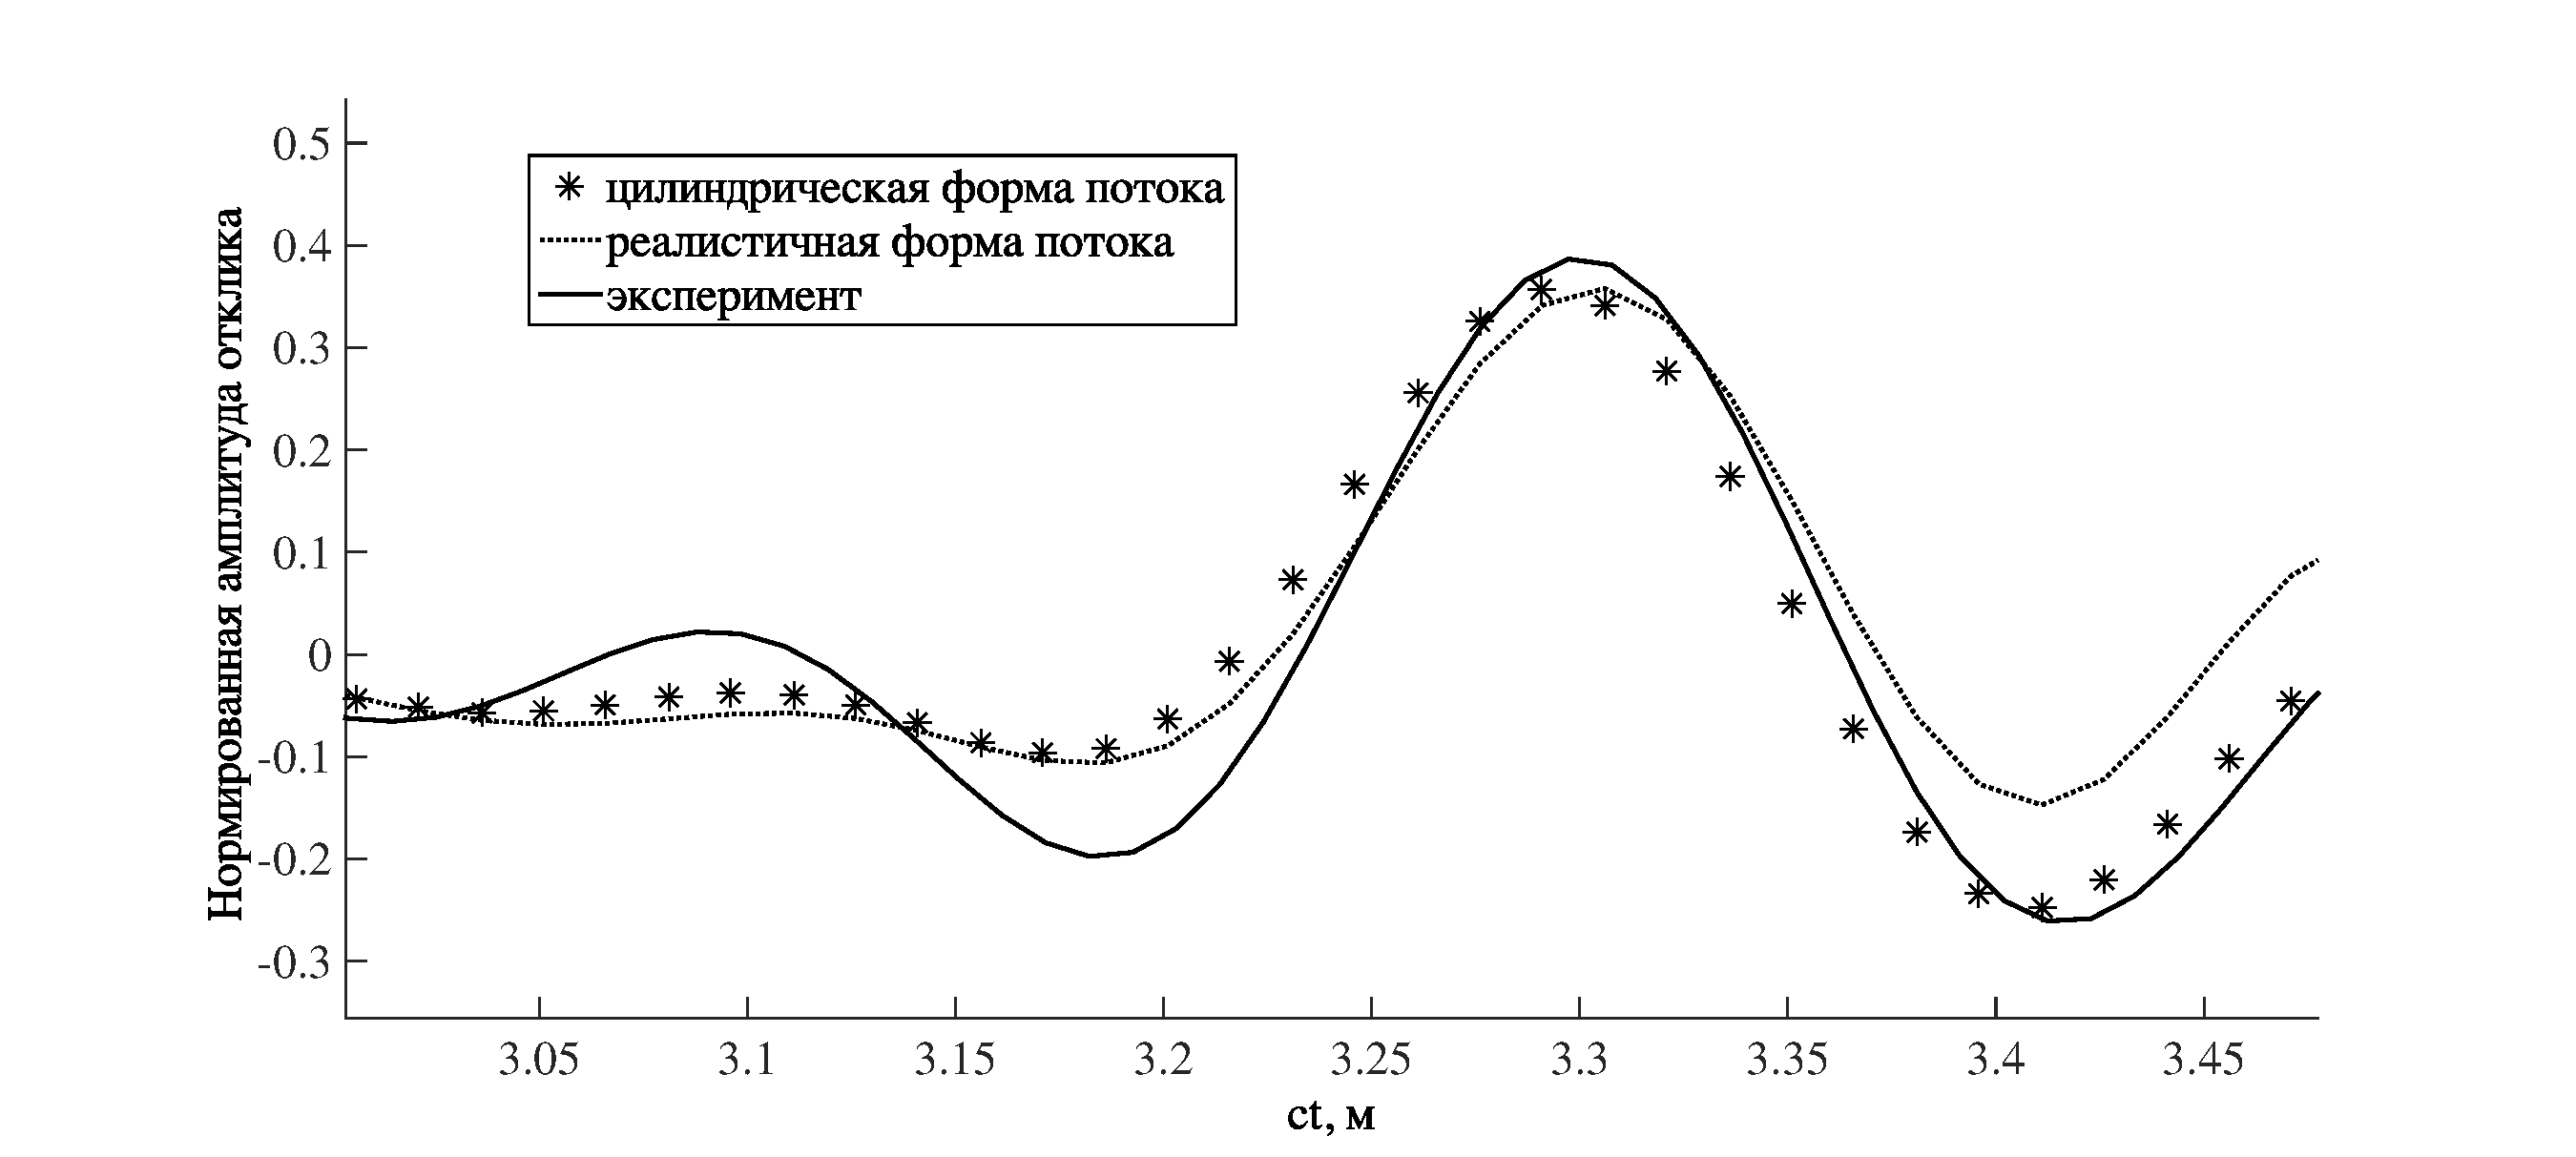
\includegraphics [scale=0.4] {ris2_11}
	\caption{Сравнение моделирования и эксперимента для микрофона 2, V = 20 м/c.}
	\label{img:ris2_11}
\end{figure}

\begin{figure}[ht]
	\centering
	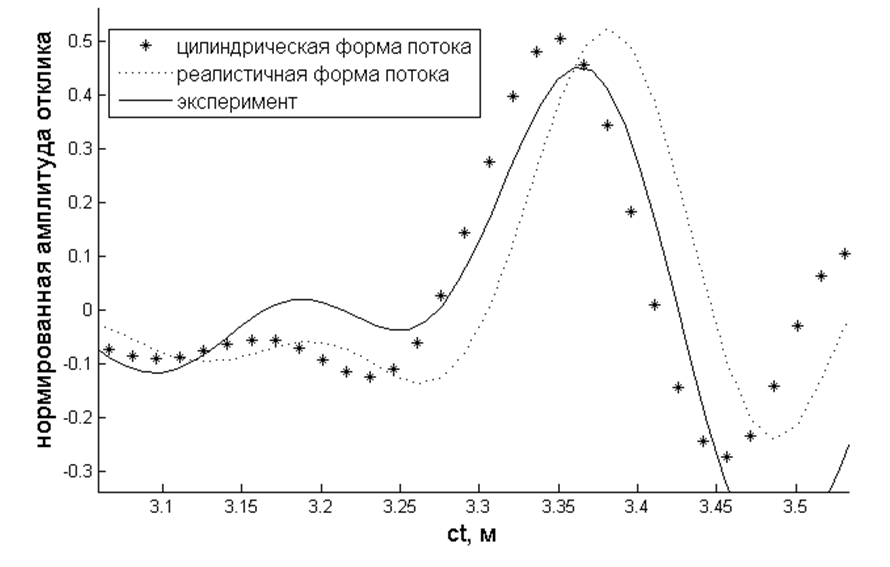
\includegraphics [scale=0.6] {ris2_12}
	\caption{Сравнение моделирования и эксперимента для микрофона 2, V = 60 м/c.}
	\label{img:ris2_12}
\end{figure}


Как видно из графиков, теоретические результаты неплохо согласуются с экспериментальными данными. Также стоит отметить, что моделирование не описывает падение амплитуды сигнала на скоростях $60$ и $80$ м/с. Это косвенно свидетельствует о том, что падение амплитуды обусловлено флуктуациями в потоке, которые здесь не учитываются.

Сигналы на микрофонах 1 и 3 (выше и ниже микрофона 2, см. Рис. \ref{img:ris2_1}) слабо отличаются от сигналов на микрофоне 2. На этих микрофонах снос выражен слабее, а фокусировка приводит не к усилению, а ослаблению амплитуды.

\section{Шумы и время накопления}
	
Стоит отметить, что "сырой" сигнал на приемном микрофоне сильно зашумлен, особенно при большой скорости потока. Использование MLS техники в данном случае может рассматриваться как эффективная противошумовая мера. А именно, квазишумовые сигналы до корреляционной обработки выглядят, как показано на (Рис. \ref{img:ris2_13}, \ref{img:ris2_14}). Полезный сигнал составляет примерно $0.1$ Па, он теряется на фоне шумов уже при скорости потока $20$ м/c (шум на микрофоне составляет 1 Па), и совсем теряется при скорости потока $80$ м/c (шум составляет 10 Па). Корреляционная обработка позволяет выделить импульсный отклик весьма хорошо до $60$ м/c (Рис. \ref{img:ris2_13}).


\begin{figure}[ht]
	\centering
	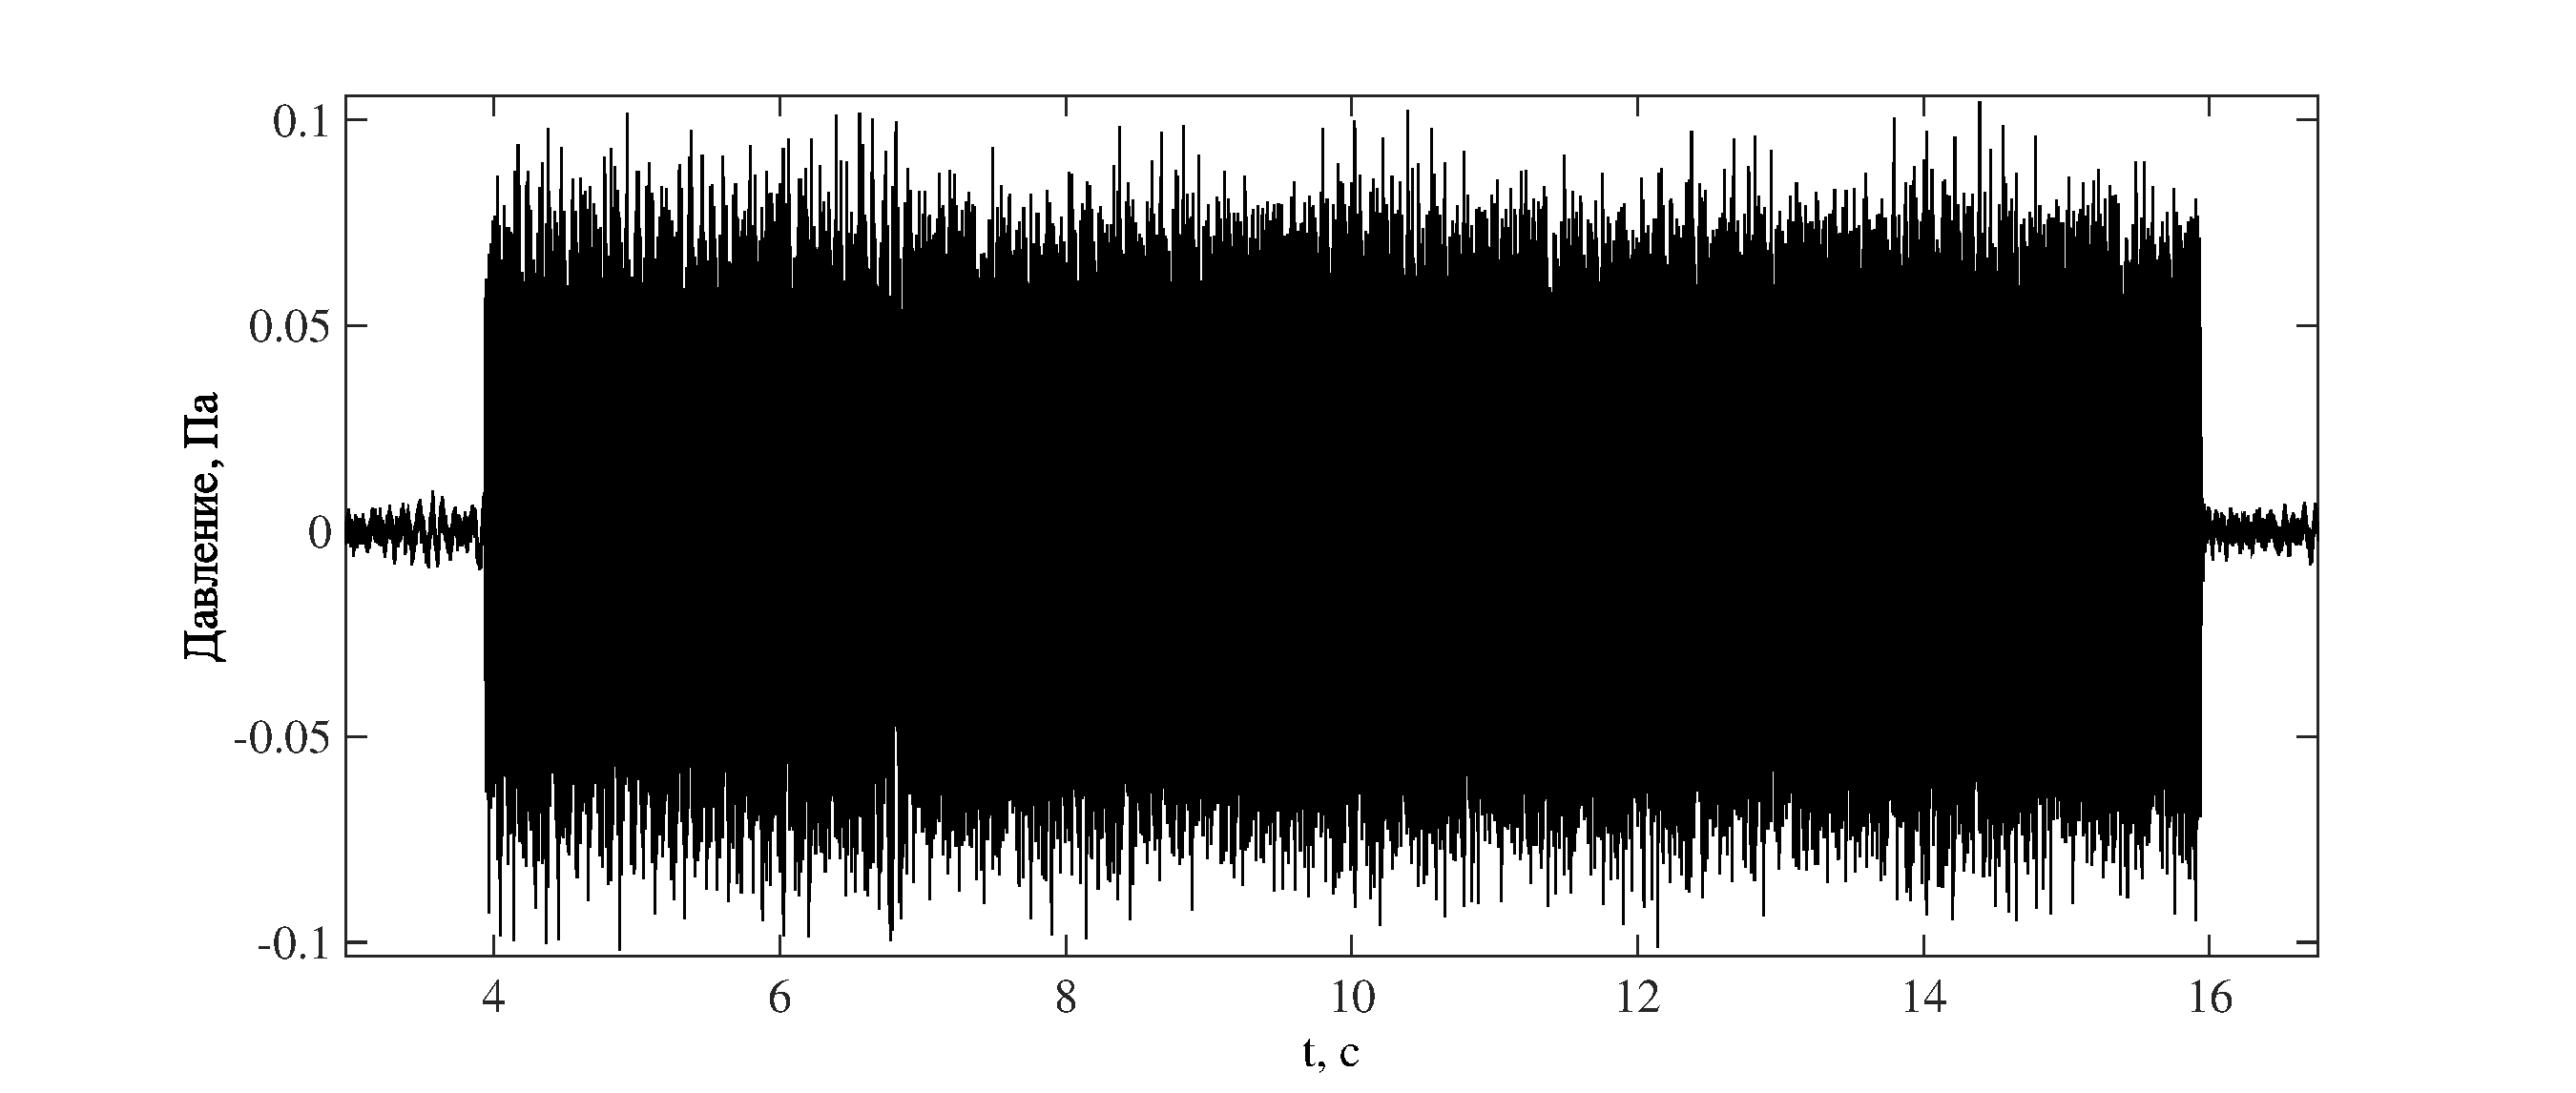
\includegraphics [scale=0.4] {ris2_13}
	\caption{Сигнал до обработки при скорости потока V = 0 м/с.}
	\label{img:ris2_13}
\end{figure}

\begin{figure}[ht]
	\centering
	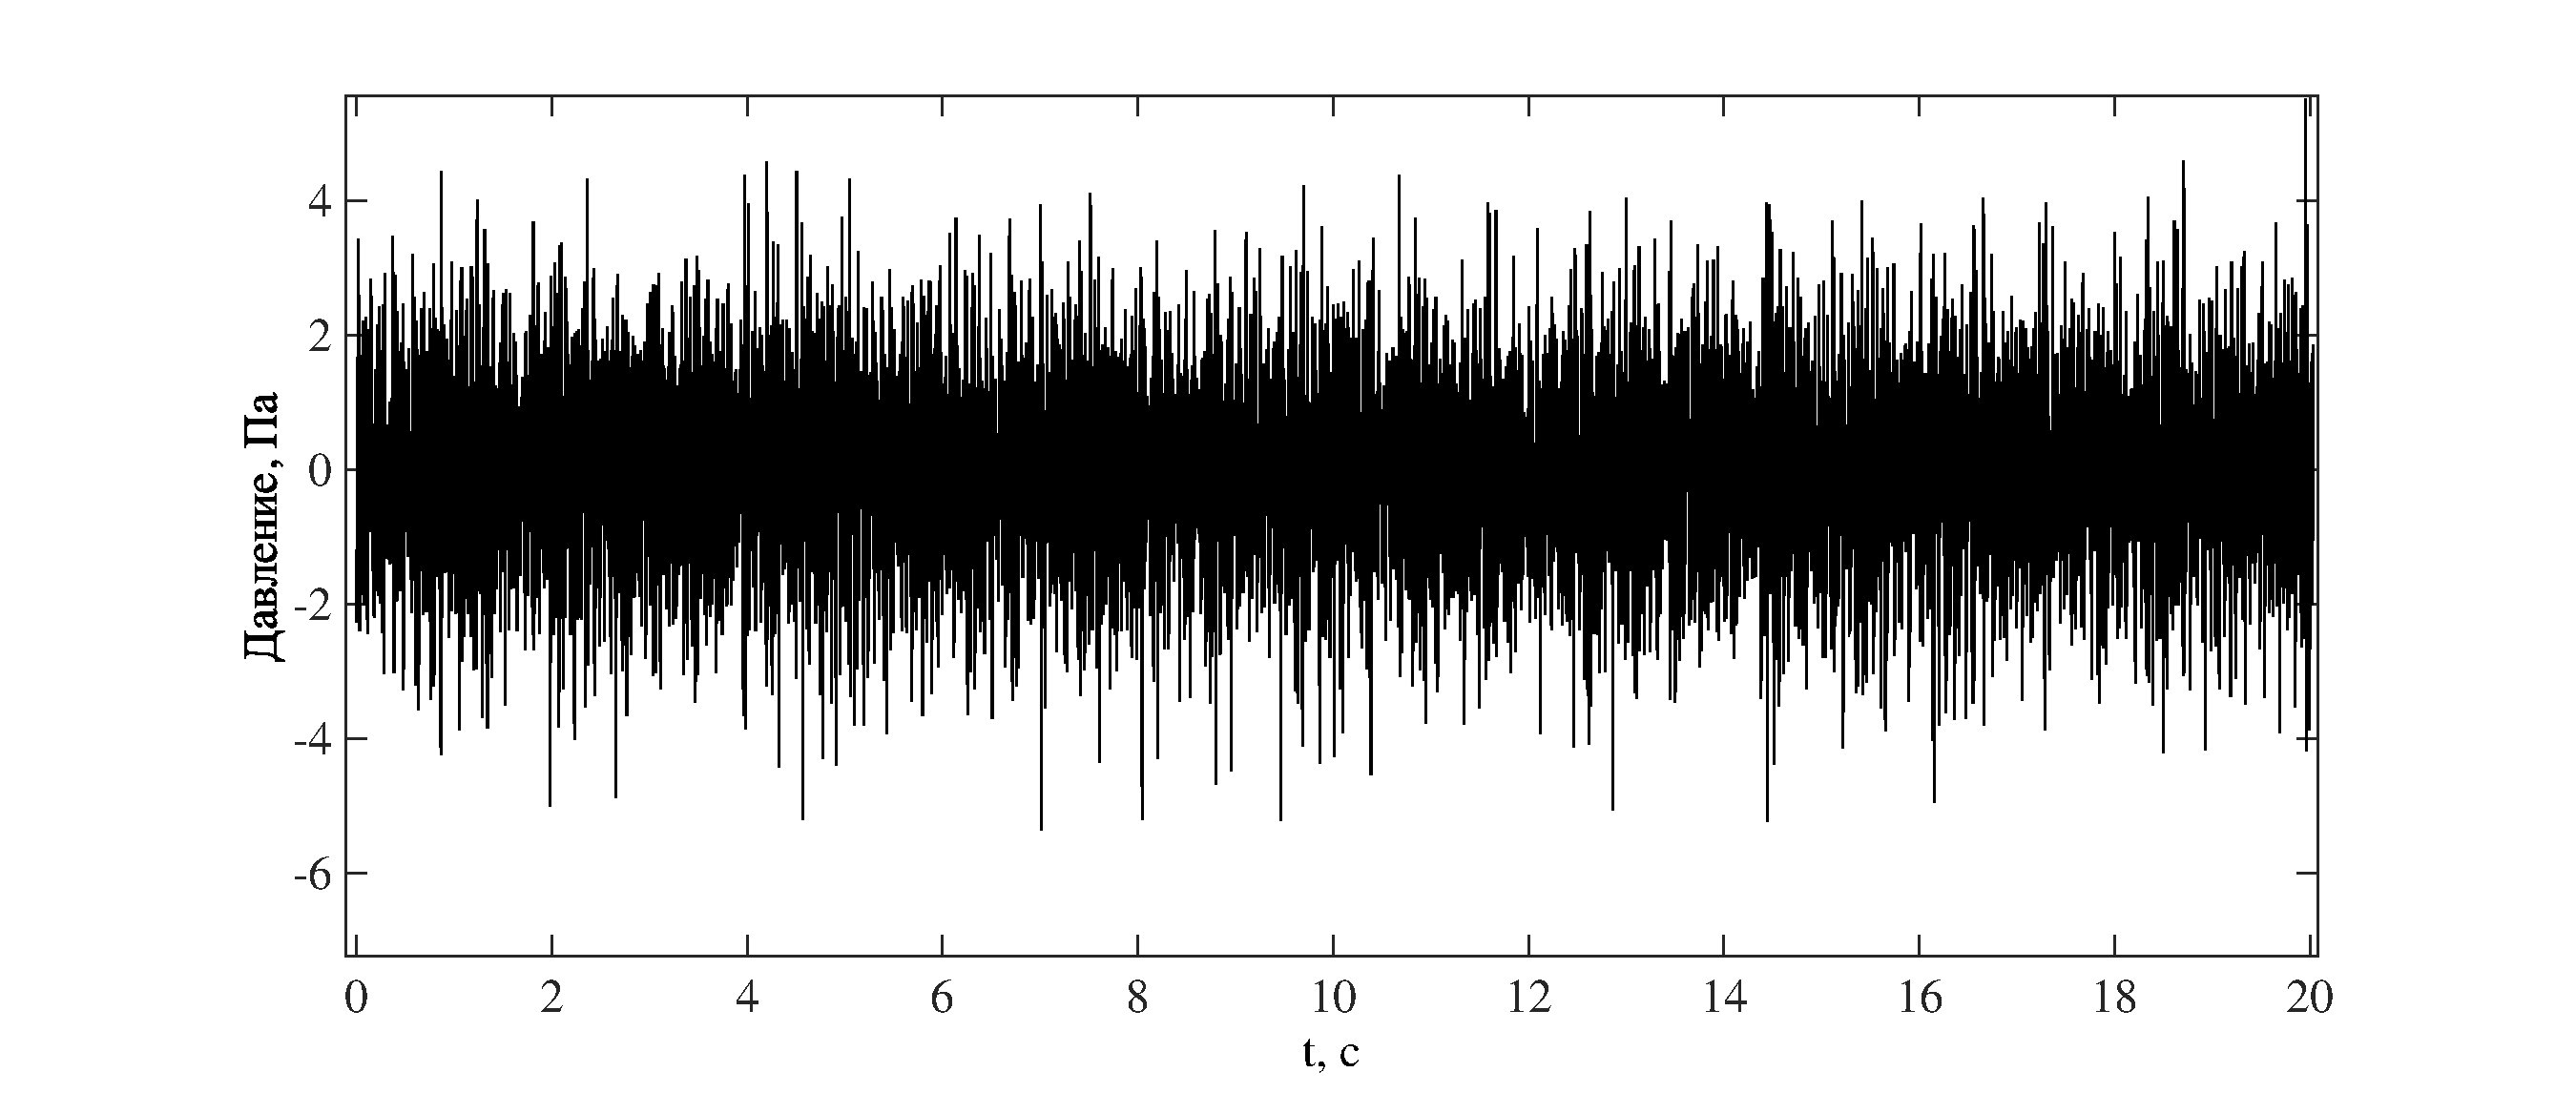
\includegraphics [scale=0.4] {ris2_14}
	\caption{Сигнал до обработки при скорости потока V = 60 м/с.}
	\label{img:ris2_14}
\end{figure}

\begin{figure}[ht]
	\centering
	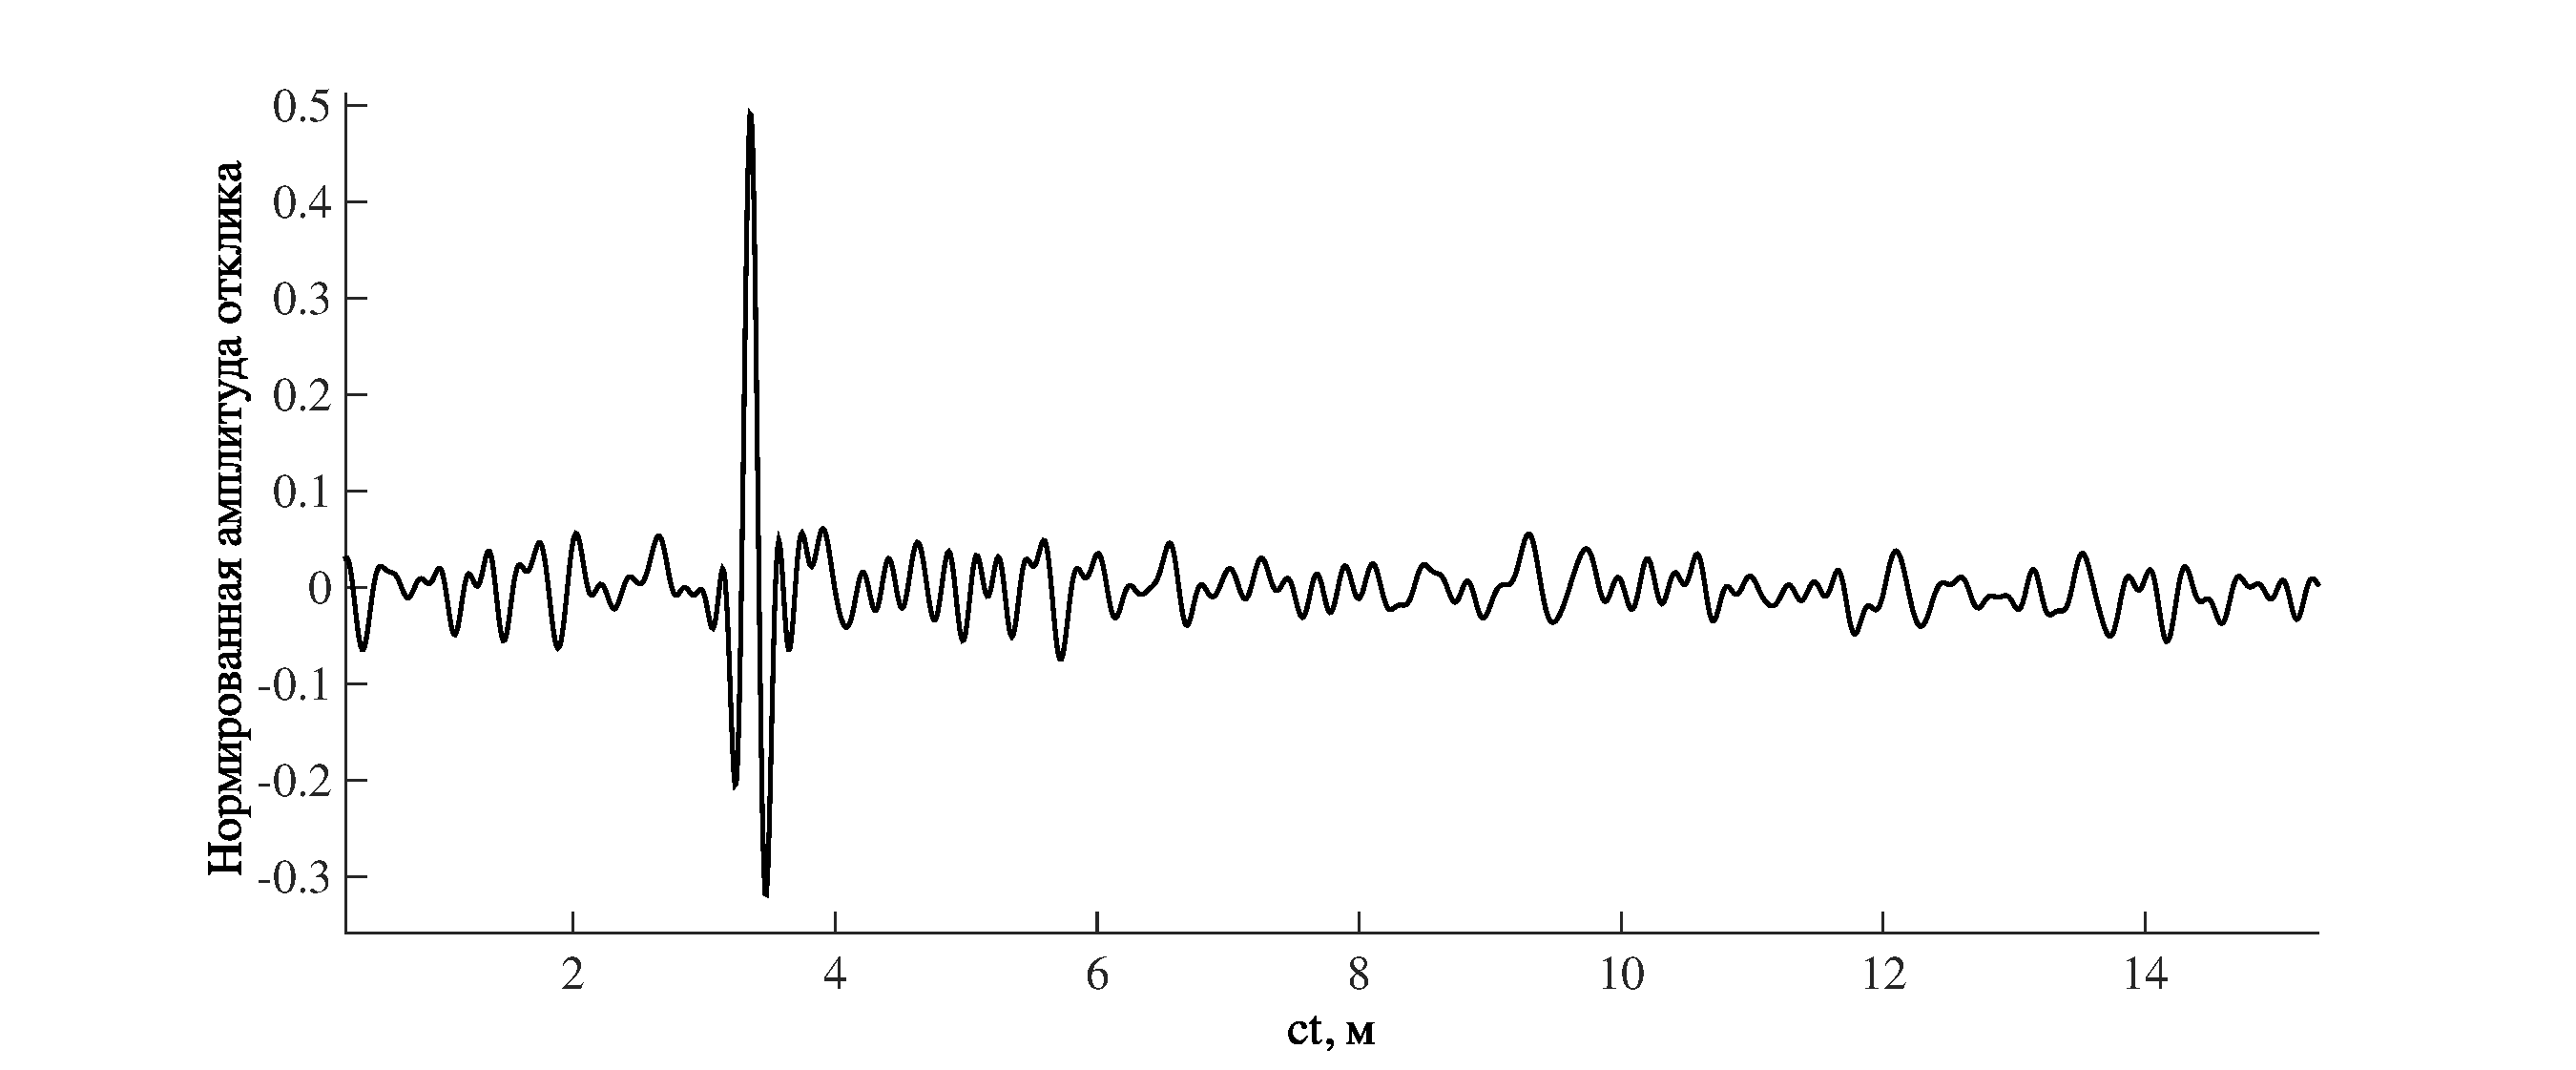
\includegraphics [scale=0.4] {ris2_15}
	\caption{Восстановленный импульсный отклик при скорости потока V = 60 м/с.}
	\label{img:ris2_15}
\end{figure}

Дальнейшее снижение шума возможно за счет увеличения времени накопления сигнала. Был проведен эксперимент по увеличению времени накопления в 3 раза. При этом средний квадрат шума снижался в 3 раза в полном соответствии с теоретическими представлениями. При работе в сильных потоках авторы предлагают увеличивать время накопления еще существеннее.

\section{Заключение}
В данной работе представлены результаты проведения прямого дифракционного эксперимента в присутствии воздушной струи. Проверялась возможность проведения измерений с использованием MLS-техники на фоне струи, создающей значительный шум. В рамках данного подхода удалось восстановить импульсный отклик, а также пронаблюдать основные эффекты, оказываемые потоком на звук: фокусировку и снос сигнала. Кроме того, был произведен теоретический расчет этих эффектов в предположении небольших чисел Маха и двух различных форм потока: цилиндрической и реалистичной, основанной на данных. Результаты расчета показали хорошее согласование с экспериментом.


\chapter{Дифракция на вытянутом теле вращения с импедансными границами. Метод граничного интегрального параболического уравнения}

В данной главе изучается задача дифракции на вытянутом теле вращения с импедансными граничными условиями. Рассматривается случай приосевого падения высокочастотной волны. Дифракционный процесс описывается с помощью метода параболического уравнения. С помощью теоремы Грина выводится граничное интегральное уравнения типа Вольтерра. Для задачи дифракции на тонком конусе с постоянным импедансом строится итерационное численное решение. Также, численные результаты сравниваются c результатами прямого дифракционного акустического эксперимента, выполненного с использованием метода M-последовательности

\section{Введение}

В этой главе рассматривается задача дифракции на вытянутом теле вращения. Иными словами, предполагается, что продольные размеры тела значительно превышают его поперечные размеры. Поле на поверхности удовлетворяет импедансным граничным условиям. Рассматривается случай приосевого падения. Также предполагается, что длины волн значительно меньше продольных размеров препятствия. При таких предположениях дифракционная задача значительно упрощается и может быть решена в рамках метода параболического уравнения.

Задачи дифракции на вытянутых телах привлекают значительное внимание исследователей. В частности, хорошо изучен случай идеальных граничных условий \cite{Andronov2011, Andronov2012, Andronov2012_2, Kirpichnikova2013, Popov2014, Engineer1998, Smyshlyaev1990, Felsen1957}. Этот случай также рассматривался авторами \cite{Shanin2011, Shanin2017}. Подробный обзор существующих методов может быть найден в \cite{Shanin2017}. К сожалению, задачи дифракции на телах вращения с импедансными граничными условиями практически не изучены. Авторам известны лишь работы, посвященные импедансному конусу \cite{Lyalinov2003, Bernard2004, Antipov2003}. В данных работах с помощью интегрального представления Конторовича-Лебедева задачу удается свести интегральному уравнению типа Фредгольма. Для случая тонкого конуса строится диаграмма направленности. В \cite{Lyalinov2009} исследовано дальнее поле вблизи поверхности конуса.

Настоящая работа является обобщением результатов, полученных в \cite{Shanin2017}, на случай импедансных граничных условий. А именно, выводится граничное интегральное уравнение в параболической постановке. Полученное уравнение относится к классу Вольтерра, что позволяет его решить с помощью метода итераций.

В работе выводятся интегральные уравнения двух типов. Уравнение первого типа, более общее, является двумерным и имеет ядро, зависящее от четырех переменных: двух координат источника и двух координат приемника на поверхности препятствия. Данное уравнение формулируется для произвольного вытянутого тела. Путем учета угловой симметрии выводится ряд одномерных уравнений для угловых мод. Эти уравнения, соответственно, справедливы только для тел вращения. При осевом падении остается только уравнение для нулевой моды, которое решается методом итераций для задачи дифракции на конусе с постоянным импедансом.

Кроме того, полученные численные и аналитические результаты сравниваются с результатами прямого акустического дифракционного эксперимента, выполненного с применением метода M-последовательности. Сравнение проводится для случая идеальных граничных условий Неймана.

\section{Постановка задачи}

\subsection{Постановка задачи для уравнения Гельмгольца}

Рассмотрим трехмерное пространство, описываемое цилиндрическими координатами $(x, r, \varphi)$. Будем считать, что $x$ — продольная координата в том смысле, что все волновые процессы происходят под малым углом к оси $x$. Пусть везде вне тела выполняется уравнение Гельмгольца:

\begin{eqnarray}
\label{eq:helmholtz}
\left(\frac{\partial^2}{\partial x^2} + \Delta_\perp + k^2\right) \tilde{u}(x, r, \varphi) = 0, \\
\Delta_\perp = \frac{1}{r} \frac{\partial}{\partial r} r \frac{\partial}{\partial r} + \frac{1}{r^2} \frac{\partial}{\partial \varphi}
\end{eqnarray}

Временная зависимость имеет форму $\exp(-i\omega t)$ и далее не выписывается. Тело вращения занимает симметричную относительно оси $x$  область $r < f(x)$. Будем обозначать поверхность тела символом $\Gamma$. Тело может быть как компактным $(X_1 \leq x \leq X_2)$, так и полубесконечным $(x \geq X_1)$. Примером тела вращения является конус:
\begin{equation}
\label{eq:straightline}
r = f(x) = \alpha x, x\geq 0.
\end{equation}

Падающая волна имеет вид:
\begin{equation}
\label{eq:inc_small_angle}
\tilde{u}^{\text{in}} = \exp\{ik(x\cos \theta + r \cos \varphi \sin \theta)\},
\end{equation}
где угол падения $\theta$ предполагается малым. 

Полное поле $\tilde{u}$ представляется в следующем виде:

\begin{equation}
\tilde{u} = \tilde{u}^{\text{in}} + \tilde{u} ^ {\text{sc}}.
\end{equation}

Здесь $\tilde{u}^{\text{sc}}$ — рассеянное поле, удовлетворяющее условиям излучения. Условия излучения формулируются в виде принципа предельного поглощения. А именно, предполагается, что волновое число $k$ имеет малую положительную мнимую часть. Следовательно, рассеянное поле затухает при $|x| \rightarrow \infty$ или $|r| \rightarrow \infty$.

На поверхности тела должны выполняться импедансные граничные условия:

\begin{equation}
\label{eq:imp_usl}
\frac{\partial \tilde{u}}{\partial \textbf{n}} = \eta \tilde{u},
\end{equation}
где $\eta$ - импеданс, $\textbf{n}$ - внешняя нормаль к поверхности тела. На импеданс накладывается условие неизлучения энергии

\begin{equation}
\label{eq:neizl}
\text{Im}\left[\eta\right] \leq 0.
\end{equation}

Если на поверхности тела имеются конические точки (такие, как вершина конуса), то в них должны удовлетворяться условия Мейкснера, заключающиеся в интегрируемости «энергии» $|\nabla \tilde{u}|^2 + |\tilde{u}|^2$ вблизи конической точки.

\subsection{Постановка задачи для параболического уравнения}

Предполагается, что тело вращения вытянуто в том смысле, в котором это понятие было введено в \cite{Shanin2017}. А именно, предполагается, что дифракционный процесс носит приосевой характер, т. е. выполнены следующие условия:

\begin{itemize}
	\item Угол падения мал: $\theta \ll 1$.
	\item Наклон поверхности меняется плавно: $\dot{f} \ll 1$. Здесь $\dot{f}$ - производная $df/dx$.
	\item Угол дифракции мал: $(\ddot{f}/k)^{1/3} \ll 1$. Здесь $\ddot{f}$ - прозводная $d^2 f/ dx^2$.
\end{itemize}

Поясним последнее условие. Продольный размер зоны Френеля определяется выражением \cite{Fok1970}:

\begin{equation}
\label{eq:long_fresnel}
\Delta x = \left(\ddot{f}\right)^{-2/3} k^{-1/3}.
\end{equation}

Угол дифракции может быть оценен как изменение наклона поверхности на $\Delta x$, т.е. как $\Delta x \ddot{f} = \left(\ddot{f}/k\right)^{1/3}$.

В соответствии с методом параболического уравнения, представим полное поле в виде

\begin{equation}
\label{eq:inc_wave}
\tilde{u}(x, r, \varphi) = e^{ikx} u(x, r, \varphi),
\end{equation}
где $u(x,r,\varphi)$  является медленной функцией $x$ по сравнению с экспоненциальным множителем. Подставляя ~\eqref{eq:inc_wave} в ~\eqref{eq:helmholtz} и пренебрегая членом с второй производной по $x$, получаем параболическое уравнение теории дифракции (ПУТД):

\begin{equation}
\label{eq:putd}
\left(\frac{\partial}{\partial x} + \frac{1}{2ik} \Delta_\perp\right) u = 0.
\end{equation}

Падающая волна ~\eqref{eq:inc_small_angle} в параболическом приближении принимает вид

\begin{equation}
\label{eq:inc_wave2}
u^{\text{in}} (x, r, \varphi) = \exp\{ ik \left(\theta r \cos \varphi  - x\theta^2 / 2 \right) \},
\end{equation}
где учтено, что $\cos \theta \approx 1 - \theta^2/2$, $\sin \theta \approx \theta$. Легко проверить, что ~\eqref{eq:inc_wave2} удовлетворяет ~\eqref{eq:putd}. В случае осевого падения $\theta = 0$ имеем

\begin{equation}
u^{\text{in}} = 1.
\end{equation}

Импедансные граничные условия ~\eqref{eq:imp_usl} переходят в

\begin{equation}
\label{eq:imp_cond2}
N\left[u\right](x, f(x), \varphi) = \eta u, \quad N \equiv \frac{\partial}{\partial r} - ik\dot{f}.
\end{equation}

Переход от $\partial/\partial n$ к $N$ подробно обсуждается в \cite{Shanin2017}. А именно, непосредственно вычисляя производную от ~\eqref{eq:inc_wave}, и пренебрегая членами порядка $\left(\dot{f}\right)^2$, получим ~\eqref{eq:imp_cond2}.

Как известно, наличие импедансных граничных условий может приводить к появлению поверхностных волн. Если их скорость существенно меньше скорости волн в среде, параболическое приближение не будет справедливым. Потребуем выполнения следующего условия

\begin{equation}
\label{eq:potrebuem_sled}
\eta/k \ll 1.
\end{equation}

Тогда скорость распространения поверхностных волн будет близка к скорости звука \cite{Korolkov2016}, и, следовательно, они будут хорошо описываться параболическим приближением. Также предполагается выполнение условия неизлучения энергии ~\eqref{eq:neizl}.


Постановка задачи для ПУТД должна быть дополнена начальным условием
\begin{equation}
u^{\text{sc}} = 0, \quad \text{при} \quad x<X_1,
\end{equation}
отражающим тот факт, что ПУТД описывает только волны, распространяющиеся в положительном направлении.

Кроме того, должны выполняться условия излучения, накладываемые в виде принципа предельного поглощения.

Наконец, требуется выполнение условий Мейкснера. А именно, вблизи конической точки требуется локальная интегрируемость следующего выражения \cite{Shanin2017}:

\begin{equation}
|\Delta_\perp u|^2 + |u|^2.
\end{equation}

\section{Вывод граничного интегрального уравнения}

\subsection{Теорема Грина для параболического уравнения}
Введем векторные обозначения для точек пространства $\textbf{r} = (x, r, \varphi)$. Определим функцию Грина как решение неоднородного параболического уравнения с источником в точке $\textbf{r}_s = (x_s, r_s, \varphi_s)$:

\begin{equation}
\label{eq:neodn_parabol}
\left(\frac{\partial}{\partial x} + \frac{1}{2ik} \Delta_\perp \right) g(\mathbf{r}, \mathbf{r_s}) = \delta(\mathbf{r}, \mathbf{r_s}),
\end{equation}
где оператор в левой части действует на компоненты вектора $\textbf{r}$, а $\delta$ — дельта-функция Дирака. Решение уравнения должно удовлетворять начальному условию, то есть должно обращаться в ноль при $x < x_s$. При помощи непосредственной подстановки в ~\eqref{eq:neodn_parabol} можно убедиться, что функция Грина при $x>x_s$ имеет следующий вид:

\begin{equation}
g(\textbf{r}, \mathbf{r_s}) = \frac{k}{2 \pi i (x-x_s)} \exp \{\frac{ik}{2} \frac{(\Delta r)^2}{x-x_s} \},
\end{equation}
где $\Delta r$ - расстояние между проекциями векторов в поперечной плоскости:

\begin{equation}
(\Delta r)^2 = r^2 + r_s^2 - 2r r_s \cos(\varphi - \varphi_s).
\end{equation}

Сформулируем теорему Грина для параболического уравнения. Пусть $\Omega$ - конечная связная область с гладкой границей $\partial \Omega$  и внешней нормалью $\textbf{n}$. Рассмотрим пару неоднородных параболических уравнений

\begin{equation}
\label{eq:eq18}
\left(\frac{\partial}{\partial x} + \frac{1}{2ik} \Delta_\perp\right) v(x, r, \varphi) = q(x, r, \varphi),
\end{equation}

\begin{equation}
\left(-\frac{\partial}{\partial x} + \frac{1}{2ik} \Delta_\perp\right) w(x, r, \varphi) = h(x, r, \varphi)
\end{equation}
для некоторых $v, q, w, h$. Отметим, что второе уравнение является комплексно сопряженным к первому, то есть описывает распространение волн в отрицательном направлении. 

Введем векторные функции:

\begin{equation}
\textbf{v}(x,y,z) = \left( ikv, \frac{\partial v}{\partial r}, \frac{1}{r} \frac{\partial v}{\partial \varphi} \right), \quad \mathbf{w}(x,y,z) = \left( -ikw, \frac{\partial w}{\partial r}, \frac{1}{r} \frac{\partial w}{\partial \varphi} \right)
\end{equation}

Наконец, сформулируем теорему Грина \cite{Shanin2017}:

\begin{equation}
\int_{\partial \Omega} [ (\mathbf{v \dot n}) w - (\mathbf{w \dot n}) v  ] dS = 2ik \int_{\Omega} [qw - hv ] dV.
\end{equation}

\subsection{Граничное интегральное уравнения для полного поля}

\begin{figure}[ht]
	\centering
	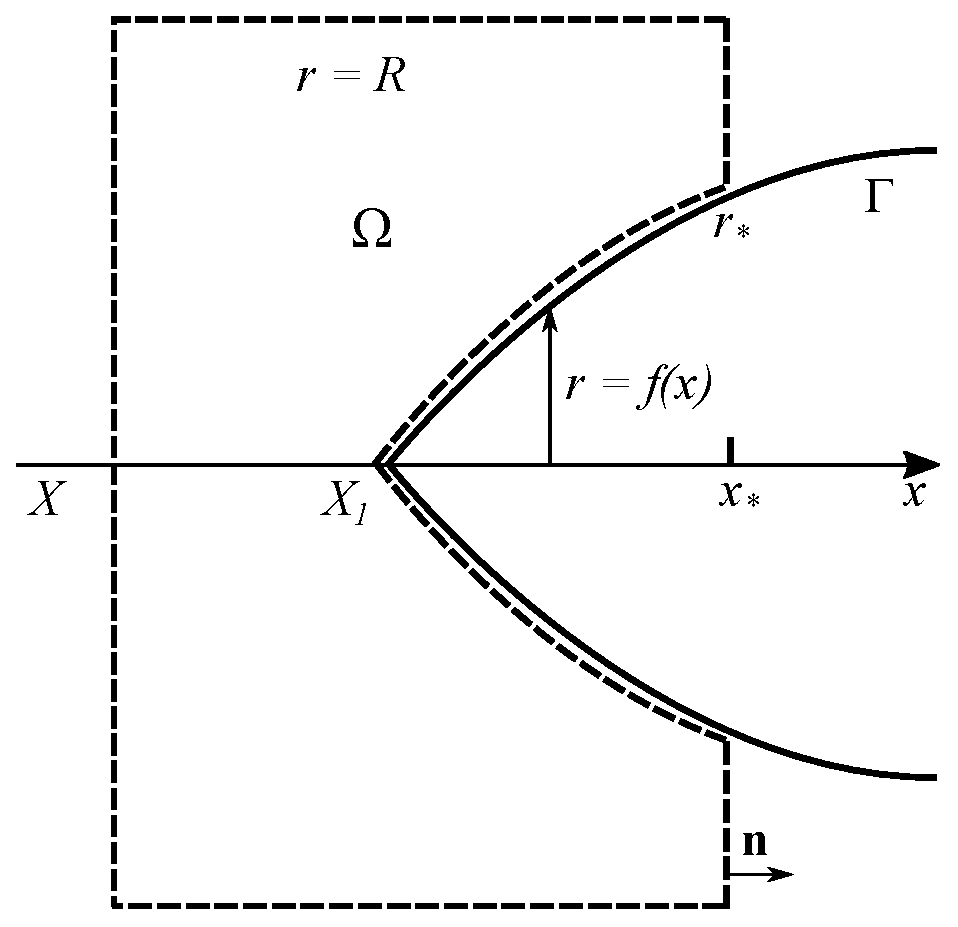
\includegraphics [scale=0.5] {ris3_1}
	\caption{Сечение области для теоремы Грина.}
	\label{img:ris3_1}
\end{figure}

Применим теорему Грина к области $\Omega$, сечение которой изображено на Рис. \ref{img:ris3_1}. Область ограничена плоскостью $x = X$, где $X < X_1$, плоскостью $x = x_*$ для некоторого $x_*$, цилиндром $r = R$, где $R \rightarrow \infty$, и поверхностью тела вращения $\Gamma$. Область $\Omega$ обладает осевой симметрией относительно оси $x$. В качестве $v$ подставим в ~\eqref{eq:eq18} рассеянное поле $u^{\text{sc}}$, а в качестве $w$ подставим $g(\mathbf{r_*, r})$, где 

\begin{equation}
r_* = (x_* + \varepsilon, f(x_* + \varepsilon), \varphi_*).
\end{equation}

Здесь $\varphi_*$ предполагается произвольным, $\varepsilon$ — малым (ниже рассматривается предел $\varepsilon \rightarrow 0$). Проводя выкладки, аналогичные таковым в \cite{Shanin2017}, получаем следующее интегральное уравнение:

\begin{multline}
\label{eq:u_sc}
U^{\text{sc}}(x_*, \varphi_*) = \frac{i}{k} \int_{0}^{2\pi} \int_{X_1}^{x_*} U^{\text{sc}}(x,\varphi) \{\bar{N}\left[W\right](x,\varphi) - \eta W(x, \varphi) \} f(x) dx d\varphi + \\
\frac{i}{k} \int_{0}^{2\pi} \int_{X_1}^{x_*} W(x, \varphi) \{ N \left[U^{\text{in}} \right] (x, \varphi)  - \eta U^{\text{in}}(x, \varphi) \} f(x) dx d\varphi,
\end{multline}
где были введены следующие обозначения:

\begin{eqnarray}
&\bar{N} \equiv \frac{\partial}{\partial r} - ik \frac{df}{dx}, \\
&U^{\text{sc}} (x, \varphi) \equiv u^{\text{sc}}(x, f(x), \varphi), \\
&U^{\text{in}} (x, \varphi) \equiv u^{\text{in}}(x, f(x), \varphi), \\
& W(x, \varphi) \equiv w(x, f(x), \varphi).
\end{eqnarray}

Введем обозначение для ядра уравнения ~\eqref{eq:u_sc}:

\begin{equation}
\label{eq:obosn_dlya_yadra}
K(x_*, \varphi_*, x, \varphi) \equiv \frac{i f(x)}{k} ( \bar{N} \left[W\right] (x,\varphi) - \eta W(x, \varphi) ).
\end{equation}

Уравнение ~\eqref{eq:u_sc} может быть упрощено. А именно, применяя теорему Грина к области $\Omega$ с функциями

$$v(r) = u^{\text{in}}(r), \quad w(r) = g(r_*, r),$$
получим интегральное соотношение:

\begin{multline}
\label{eq:u_in}
U^{\text{in}}(x_*, \varphi_*) = \frac{i}{k} \int_{0}^{2\pi} \int_{X_1}^{x_*} U^{\text{in}}(x,\varphi) \{\bar{N}\left[W\right](x,\varphi) - \eta W(x, \varphi) \} f(x) dx d\varphi + \\
\frac{i}{k} \int_{0}^{2\pi} \int_{X_1}^{x_*} W(x, \varphi) \{ N \left[U^{\text{in}} \right] (x, \varphi)  - \eta U^{\text{in}}(x, \varphi) \} f(x) dx d\varphi + 2 U^{\text{in}}(x_*, \varphi_*),
\end{multline}

Складывая ~\eqref{eq:u_sc} и ~\eqref{eq:u_in}, получим уравнение для полного поля $U = U^{\text{sc}} + U^{\text{in}}$  на поверхности тела:

\begin{equation}
\label{eq:main_intur}
U(x_*, \varphi_*) = \int_{0}^{2 \pi} \int_{X_1}^{x_*} K(x_*, \varphi_*, x, \varphi) U(x, \varphi) dx d\varphi + 2 U^\text{in} (x_*, \varphi_*).
\end{equation}

Ядро ~\eqref{eq:u_sc} дается следующим выражением:

\begin{equation}
\label{eq:yadro_intura}
K(x_*, \varphi_*, x, \varphi) = \frac{ikf(x)}{2 \pi} \left( \frac{1}{ik} \frac{ik\dot{f}(x) - \eta}{x_* - x}  + \frac{f(x) - f(x_*) \cos(\varphi - \varphi_*)}{(x_* - x)^2}\right) \times \exp \{ \frac{ik}{2} \frac{(f(x))^2  + (f(x_*))^2 - 2f(x_*) f(x_*) \cos(\varphi - \varphi_*) }{x_* - x} \}
\end{equation}

Уравнение ~\eqref{eq:main_intur} является уравнением Вольтерра по переменной $x$ и уравнением с разностным ядром по переменной $\varphi$.

\subsection{Граничное интегральное уравнение для угловых мод}

Воспользуемся осевой симметрией задачи. Представим падающее и полное поля на поверхности тела в виде рядов Фурье:

\begin{equation}
\label{eq:fourier_in_full}
U^{\text{in}}(x, \varphi) = \sum_{n = -\infty}^{\infty} U^{\text{in}}_n (x) e^{in \varphi}, \quad U(x,\varphi) = \sum_{n = -\infty}^{\infty} U_n(x) e^{in\varphi}.
\end{equation}
Функции $U_n$  удовлетворяют следующим интегральным уравнениям:

\begin{equation}
U_n(x_*) = \int_{X_1}^{x_*} K_n(x_*, x) U_n(x) dx + 2 U^{\text{in}} (x_*),
\end{equation}
где
\begin{equation}
K_n(x_*, x) = \int_{0}^{2 \pi} K(x_*, \varphi, x, 0) e^{-in\varphi} d\varphi.
\end{equation}

Используя ~\eqref{eq:yadro_intura}, можно получить явное выражение для $K_n(x_*, x)$:

\begin{equation}
K_n(x) = \frac{-(-i)^{n+1}}{(x_* - x)^2} \exp \{ \frac{ik}{2} \frac{r_*^2 + r^2}{x_* - x} \} \left[ \left(r + (x_* - x) \left( \frac{df}{dx} - \frac{\eta}{ik} \right) \right)J_n(\frac{k r_* r}{x_* - x}) - \frac{ir_*}{2} \left( J_{n-1}\left(\frac{kr_*r}{x_*-x}\right) - J_{n+1}\left(\frac{k r_* r}{x_*-x}\right)  \right)\right],
\end{equation}
где $r = f(x)$, $r_* = f(x_*)$, $J_n$ - функция Бесселя первого рода.
Стоит отметить, что по аналогии с \cite{Shanin2017} для конечного тела вращения может быть получено выражение для диаграммы направленности и доказана оптическая теорема.

\section{Дифракция на импедансном конусе при осевом падении}

\subsection{Граничное интегральное уравнение для конической задачи при осевом падении}

Рассмотрим конус, для которого $X_1 = 0$, т. е. вершина конуса находится в начале координат, как показано на Рис. \ref{img:ris3_2}. Профиль конуса представляет собой прямую линию ~\eqref{eq:straightline}, где $\alpha$ является тангенсом угла между осью конуса и его образующей. Предполагается, что $\alpha \ll 1$.
 
 \begin{figure}[ht]
 	\centering
 	\includegraphics [scale=0.5] {ris3_2}
 	\caption{Геометрия задачи дифракции на конусе.}
 	\label{img:ris3_2}
 \end{figure}
 
Пусть падающая волна распространяется вдоль оси $x$, то есть имеет вид ~\eqref{eq:putd}. В этом случае полное поле обладает осевой симметрией и описывается нулевой компонентой ряда ~\eqref{eq:fourier_in_full}:
$$U(x, \varphi) = U_0(x) = U(x).$$

Тогда задача сводится к одномерному интегральному уравнению:

\begin{equation}
\label{eq:big_int_eq}
U(x_*) = \int_{0}^{x_*} K_0(x_*, x) U(x) dx + 2
\end{equation}
с ядром
\begin{equation}
K_0 = \frac{ik \alpha^2 x_* x}{(x_* - x)^2} \exp \{ \frac{ik \alpha^2}{2} \frac{x_*^2 + x^2}{x_* - x} \} \times \left[  J_0\left( k \alpha^2 \frac{x x_*}{x_* - x} \right) + i J_1\left( k \alpha^2 \frac{x x_*}{x_* - x} \right) - \frac{\eta (x_* - x)}{ikx_* \alpha}J_0 \left(k \alpha^2 \frac{x x_*}{x_* - x}\right)  \right].
\end{equation}

\subsection{Случай разделяющихся переменных}

Пусть импеданс меняется обратно пропорционально $x$:

\begin{equation}
\label{eq:imp_obr_prop}
\eta = \frac{\tilde{\eta}}{x}.
\end{equation}

Тогда задача для параболического уравнения может быть решена с помощью метода разделения переменных. Перейдем в систему координат $(x, \rho, \varphi)$ с

\begin{equation}
\rho = r/x,
\end{equation}
и введем новую полевую переменную $\hat{u}$:

\begin{equation}
u(x, \rho x, \varphi) = \Xi^{-1} (x, \rho) \hat{u}(x, \rho, \varphi), \quad \Xi(x, \rho) \equiv kx \exp \{ -ikx\rho^2/2 \}.
\end{equation}

Уравнение ~\eqref{eq:putd} переходит в

\begin{equation}
\label{eq:putd_perehodit_v}
\left( \frac{\partial }{\partial x} + \frac{1}{2ikx^2} \left( \frac{1}{\rho} \frac{\partial }{\partial \rho} \left( \rho \frac{\partial}{\partial \rho} \right)  + \frac{1}{\rho^2} \frac{\partial^2}{\partial \varphi^2} \right) \right) \hat{u} = 0,
\end{equation}
а граничное условие ~\eqref{eq:imp_usl} переходит в
\begin{equation}
\label{eq:gu_2}
\frac{1}{x} \frac{\partial \hat{u}}{\partial \rho} (x, \alpha, \varphi) = \eta \hat{u}.
\end{equation}

При выполнении ~\eqref{eq:imp_obr_prop} условие ~\eqref{eq:gu_2} переходит в 

\begin{equation}
\frac{\partial \hat{u}}{\partial \rho} (x, \alpha, \varphi) = \tilde{\eta} \hat{u}
\end{equation}
и, следовательно, переменные разделяются.

Представим полное поле в виде 

$$\hat{u} = \hat{u}^{\text{sc}} + \hat{u}^{\text{in}}, \quad \hat{u}^{\text{in}} = \Xi(x, \rho).$$

Разделяя переменные в ~\eqref{eq:putd_perehodit_v}, получим следующее представление для рассеянного поля:

\begin{equation}
\label{eq:u_sc_hat}
\hat{u}^{\text{sc}} = \int C(\lambda) H_0^1 (\sqrt{\lambda} \rho) \exp \left( i\frac{\lambda}{2kx} \right) d\lambda,
\end{equation}
где $H_0^1$ — функция Ханкеля 1-го рода, а $C(\lambda)$ и контур интегрирования подлежат определению. Для определения $C(\lambda)$ подставим ~\eqref{eq:u_sc_hat} в ~\eqref{eq:gu_2}, и воспользуемся известным соотношением из теории Бесселевых функций \cite{Gradstein1963}:

\begin{equation}
kx \exp \{ \frac{-ikx\rho^2}{2} \} = -\frac{i}{2} \int_{0}^{\infty} \exp \{ \frac{i\lambda}{2kx} \} J_0(\sqrt{\lambda} \rho) d \lambda
\end{equation}
и получим:

\begin{equation}
C(\lambda) = \frac{i}{2} \frac{\eta J_0(\sqrt{\lambda} \alpha) - \dot{J}_0(\sqrt{\lambda} \alpha) \sqrt{\lambda}}{\eta H^{(1)}_0(\sqrt{\lambda} \alpha) - \dot{H}^{(1)}_0(\sqrt{\lambda} \alpha) \sqrt{\lambda}},
\end{equation}
где были введены следующие обозначения:

\begin{equation}
\frac{d J_0(\sqrt{\lambda} \rho)}{d (\sqrt{\lambda} \rho)} \equiv \dot{J}_0 (\sqrt{\lambda} \rho), \quad 
\frac{dH_0^{(1)}(\sqrt{\lambda} \rho)}{d (\sqrt{\lambda} \rho)} \equiv \dot{H}^{(1)}_0 (\sqrt{\lambda} \rho).
\end{equation}

Таким образом, рассеянное поле   дается следующим выражением:

\begin{equation}
\label{eq:u_sc_hat2}
\hat{u}^{\text{sc}} = \frac{i}{2kx} \exp \left( \frac{ik\rho^2 x}{2} \right) \int_{0}^{\infty} \frac{\eta J_0 (\sqrt{\lambda} \alpha) - \dot{J}_0 (\sqrt{\lambda} \alpha)}{\eta H_0^{(1)} (\sqrt{\lambda} \alpha) - \dot{H}_0^{(1)} (\sqrt{\lambda} \alpha)} H_0^{(1)} (\sqrt{\lambda} \rho) \exp \left(i \frac{\lambda}{2kx}\right) d\lambda.
\end{equation}

Данный ответ можно получить и непосредственно из \textbf{(32)}. Действительно, интегральное уравнение в данном случае сводится к уравнению с разностным ядром при помощи замены $x \rightarrow 1/\tau$. Решение, соответственно, строится с помощью интегрального преобразования Фурье. Аналогичные выкладки были проделаны авторами в \cite{Shanin2017}.

Стоит заметить, что импеданс в данном случае достигает больших значений при малых $x$ и, следовательно, условие ~\eqref{eq:potrebuem_sled} нарушается вблизи носика. Таким образом, формула ~\eqref{eq:u_sc_hat2} является только модельным решением для параболического уравнения. Ниже формула ~\eqref{eq:u_sc_hat2} будет использована для верификации метода численного интегрирования уравнения ~\eqref{eq:big_int_eq}. 

Также стоит отметить, что аналогичный случай разделяющихся переменных для уравнения Гельмгольца рассмотрен в \cite{Felsen}.

\subsection{Численное решение уравнения ~\eqref{eq:big_int_eq}}

\subsubsection{Случай переменного импеданса ~\eqref{eq:imp_obr_prop}}

При малых $x$ граничные условия в уравнении ~\eqref{eq:big_int_eq} близки к идеальным условиям Дирихле. Можно показать, что граничное интегральное уравнение для задачи Дирихле является уравнением Вольтерра 1-го рода, а такое уравнение, как известно, не может быть решено методом итераций. Следовательно, метод итераций не может быть применен и к уравнению ~\eqref{eq:big_int_eq}.

Будем решать ~\eqref{eq:big_int_eq}, заменяя интеграл в правой части его дискретным аналогом и сводя интегральное уравнение к системе линейных уравнений. А именно, будем искать решение, аппроксимируя $U$ кусочно-линейными функциями \cite{Zenkevitz}:

\begin{equation}
N_i(x) = 
\begin{cases}
0, &x_{i-1} > x,\\
(x-x_{i-1})/(x_i - x_{i-1}), &x_i > x> x_{i-1},\\
(x_{i+1}-x)/(x_{i+1} - x_{i}), &x_{i+1} > x > x_{i},\\
0, &x>x_{i+1}.
\end{cases}
\end{equation}

Индекс $i$ пробегает значения от $1$ до $M$, где $M$ - число базисных функций. Поле $U$ ищется в виде:

\begin{equation}
\label{eq:eq46}
U(x) \approx \sum_{i=1}^{M} U_i N_i(x),
\end{equation}
где $U_i$ - неизвестные числа подлежащие определению. Подставляя \textbf{(46)} в \textbf{(32)}, получим следующую систему линейных уравнений:

\begin{equation}
\label{eq:eq47}
U_i = \sum_{i=1}^{M} K_{ij} U_j +2, \quad \text{где} \quad K_{ij} = \int_{0}^{x_i} K_0 (x_i, x) N_j(x) dx.
\end{equation}

Для корректного вычисления матричных элементов $K_{ij}$ необходимо учитывать поведение ядра $K_0(x_*, x)$ вблизи особой точки $x_* = x$. Используя асимптотические формулы для функций Бесселя большого аргумента, можно показать, что ядро имеет особенности двух типов. Первая особенность имеет осциллирующий характер:

\begin{equation}
K_0^{\alpha}(x_*, x) \sim \sqrt{\frac{x x_*}{(x_* - x)^3}} \left(1+ \frac{i(x-x_*)}{8k \alpha^2 x x_*} \right) \exp \{ \frac{ik\alpha^2}{2} \frac{(x_*-x)^2}{x_* - x} \}
\end{equation}

Вторая особенность является интегрируемой:

\begin{equation}
K_0^b(x_*,x) \sim \sqrt{\frac{1}{x x_* (x_* - x)}} \exp \{ \frac{ik \alpha^2}{2} (x_* - x) \}.
\end{equation}

Для вычисления интеграла от $K_0^{a}(x_*, x)$ контур интегрирования деформировался в верхнюю полуплоскость. Для вычисления $K_0^{b}(x_*, x)$ применялся метод вычитания сингулярности \textbf{[20]}. После регуляризации матричные элементы $K_{ij}$ вычислялись с помощью метода трапеций. На (Рис. \ref{img:ris3_3}) представлен результат решения системы ~\eqref{eq:eq47} и приведено точное решение ~\eqref{eq:u_sc_hat2}.


 \begin{figure}[ht]
	\centering
	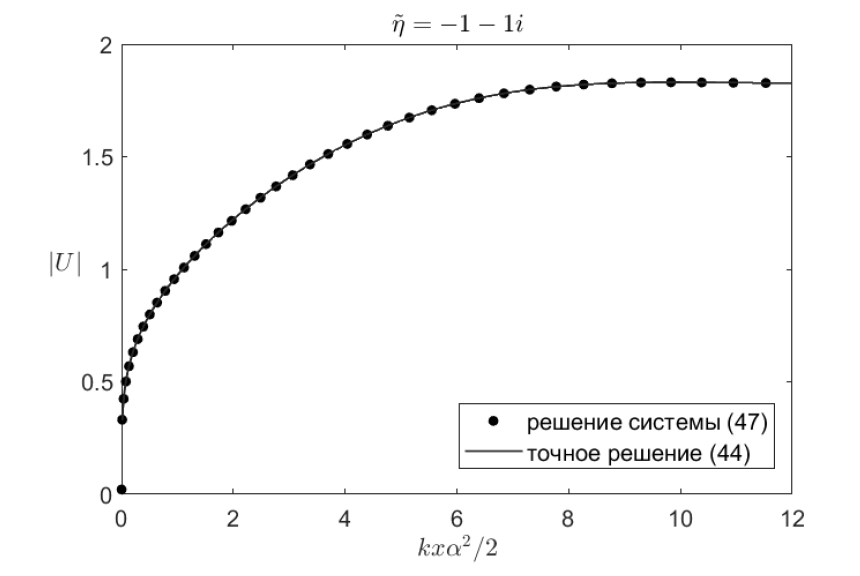
\includegraphics [scale=0.5] {ris3_3}
	\caption{Численное решение для случая переменного импеданса.}
	\label{img:ris3_3}
\end{figure}


\subsubsection{Случай постоянного импеданса}

При постоянном импедансе уравнение ~\eqref{eq:big_int_eq} может быть решено методом итераций. А именно, будем решать следующую итерационную задачу:

\begin{equation}
U(x) = \sum_{n=0}^{\infty} U^{(n)}(x),
\end{equation}

\begin{equation}
U^{(0)}(x) = 2 U^{\text{in}}(x) = 2,
\end{equation}

\begin{equation}
U^{(n+1)}(x_*) = \int_{0}^{x_*} K_0(x_*, x) U^{(n)}(x) dx, \quad n>0.
\end{equation}

Результат итерационного решения приведен на (Рис. \ref{img:ris3_4}). Как можно видеть из графиков, для достижения приемлемой точности достаточно совершить 10-15 итераций.

 \begin{figure}[ht]
	\centering
	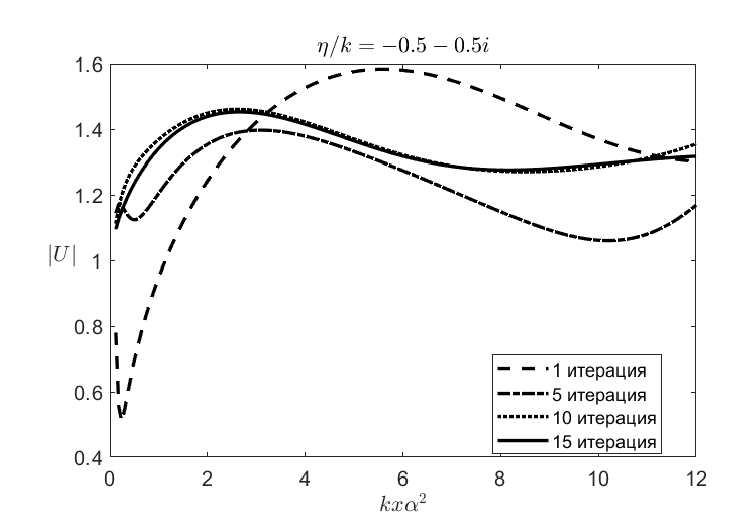
\includegraphics [scale=0.5] {ris3_4}
	\caption{Итерационное решение для случая постоянного импеданса.}
	\label{img:ris3_4}
\end{figure}

\section{Прямой дифракционный эксперимент на идеально жестком конусе}

Для случая идеально жесткого конуса, т. е. при $\eta = 0$, уравнение \textbf{(26)} было проверено экспериментально. Узкий (угол при вершине $2\alpha = 5.5$ градусов) цельный дюралюминиевый конус круглого сечения длиной 1 метр был подвешен в воздухе. Маленький (характерный размер около 1 см) микрофон был помещен на его поверхности. Конус облучался при помощи точечного по сравнению с длиной волны источника (использовался арматурный источник Knowles RAB-32257 с характерным размером около 1 см) с разных сторон так, чтобы микрофон попадал в освещенную источником или затененную конусом область Рис. \ref{img:ris3_5}.

\begin{figure}[ht]
	\centering
	\includegraphics [scale=0.5] {ris3_5}
	\caption{Схема эксперимента.}
	\label{img:ris3_5}
\end{figure}

Эксперимент проводился при помощи метода М-последовательности: конус облучался псевдослучайным сигналом с частотами 1 кГц – 10 кГц, и из корреляции между псевдослучайным сигналом и выходным сигналом с микрофона вычислялся импульсный отклик системы \cite{ValyaevMLS}. После накладывания маски во временной области при помощи преобразования Фурье вычислялся частотный отклик.

\subsection{Численное решение уравнения ~\eqref{eq:obosn_dlya_yadra}}

После аппроксимации поля на поверхности $U$ кусочно-линейными функциями \textbf{(45)}, оно представляется в виде:

\begin{equation}
\label{eq:sum_form_fun}
U(x, \varphi) \approx \sum_{i=1}^{M} U_i(\varphi) N_i(x),
\end{equation}
где $U_i(\varphi)$ - неизвестные искомые функции, имеющие угловую зависимость. Подставив ~\eqref{eq:sum_form_fun} в \textbf{26}, получим систему интегральных уравнений:

\begin{equation}
U_i(\varphi_*) = \sum_{j=1}^{M} \int_{0}^{2 \pi} K_{ij} (\varphi_*, \varphi) U_j(\varphi) d\varphi + 2 U_i^{\text{in}}(\varphi_*),
\end{equation}
где индекс $i = 1, \dots M$,

\begin{equation}
U^{\text{in}}_i(\varphi_*) = U^{\text{in}}(x_i, \varphi_*),
\end{equation}

\begin{equation}
K_{ij}(\varphi_*, \varphi) = \int_{0}^{x_i} K(x_i, \varphi_*, x, \varphi) N_j(x) dx.
\end{equation}

Подынтегральное выражение в \textbf{(54)} осциллирует около точки $x = x_i$, что может вызвать численную ошибку. Как и в случае вычисления интеграла от \textbf{(46)}, сместим контур интегрирования в верхнюю полуплоскость так, чтобы ядро $K$ экспоненциально спадало. Затем дискретизуем систему \textbf{(52)} конечными разностями и решим ее методом итераций.

\subsection{Результаты эксперимента и сравнение с решением (54)}

\subsubsection{Осевое падение}

В случае осевого падения $(r_s = 0)$ дифрагированное поле практически отсутствовало. Поле, измеренное на поверхности конуса, было близко к полю, измеренному на аналогичном расстоянии от источника в отсутствие конуса. Этот результат можно качественно объяснить с помощью метода зон Френеля для заданного источника и приемника \cite{Kravtsov}. Дифракция предполагается значительной, если препятствие покрывается несколькими зонами Френеля по отношению к координатам источника и приемника. Оценим разность прямого пути от источника к приемнику и пути луча, дифрагированного на конусе Рис. \ref{img:ris3_6}:

 \begin{figure}[ht]
	\centering
	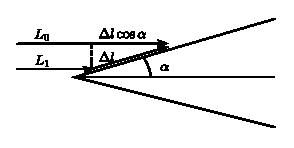
\includegraphics [scale=0.6] {ris3_6}
	\caption{Иллюстрация к оценке размера зоны Френеля.}
	\label{img:ris3_6}
\end{figure}ы

\begin{equation}
L_1 - L_0 = \Delta l(1 - \cos \alpha) \approx \Delta \alpha^2/2.
\end{equation}

Размер первой зоны Френеля $\Delta l$ можно найти, приравняв разность путей к половине длины волны:

\begin{equation}
\Delta l = \lambda/ \alpha^2.
\end{equation}

В эксперименте использовались частоты 1-10 кГц. Соответственно, размер зоны Френеля будет минимален на высоких частотах. Для конуса, исследуемого в эксперименте с углом $\alpha$ равным 2.75 градуса, минимальное значение величины $\Delta l$ может быть оценено как $(330/10^4)/(2.75\times \pi / 180)^2 \approx 14$, что в 14 раз больше длины
конуса. Следовательно, при осевом падении на конусе укладывается меньше одной зоны Френеля. Иными словами, при осевом падении данный конус представляет собой препятствие малых размеров, слабо возмущающее волновое поле. 

Отметим, что аналогичный результат можно получить, непосредственно решая уравнение \textbf{(32)}.

\subsubsection{Неосевое падение}

Используя оценку, аналогичную \textbf{(58)}, можно показать, что дифракционный процесс становится более заметным, когда источник смещается с оси конуса. В данном разделе предоставляется экспериментальное подтверждение этому факту. Результаты эксперимента для шести положений источника $y_s = \pm 0.5, \pm 0.3, \pm 0.1$ м, $x_s = -1$ м в сравнении с численным решением уравнения \textbf{(54)} показаны на \textbf{Рис. 7, 8, 9}. Микрофон был размещен на поверхности конуса в точке с продольной координатой $x = 0.8$ м, как показано на \textbf{Рис. 5}. На графиках представлены модули величины $|U/U^{\text{in}}|$, чтобы исключить геометрическое затухание поля.

\begin{figure}[ht]
	\centering
	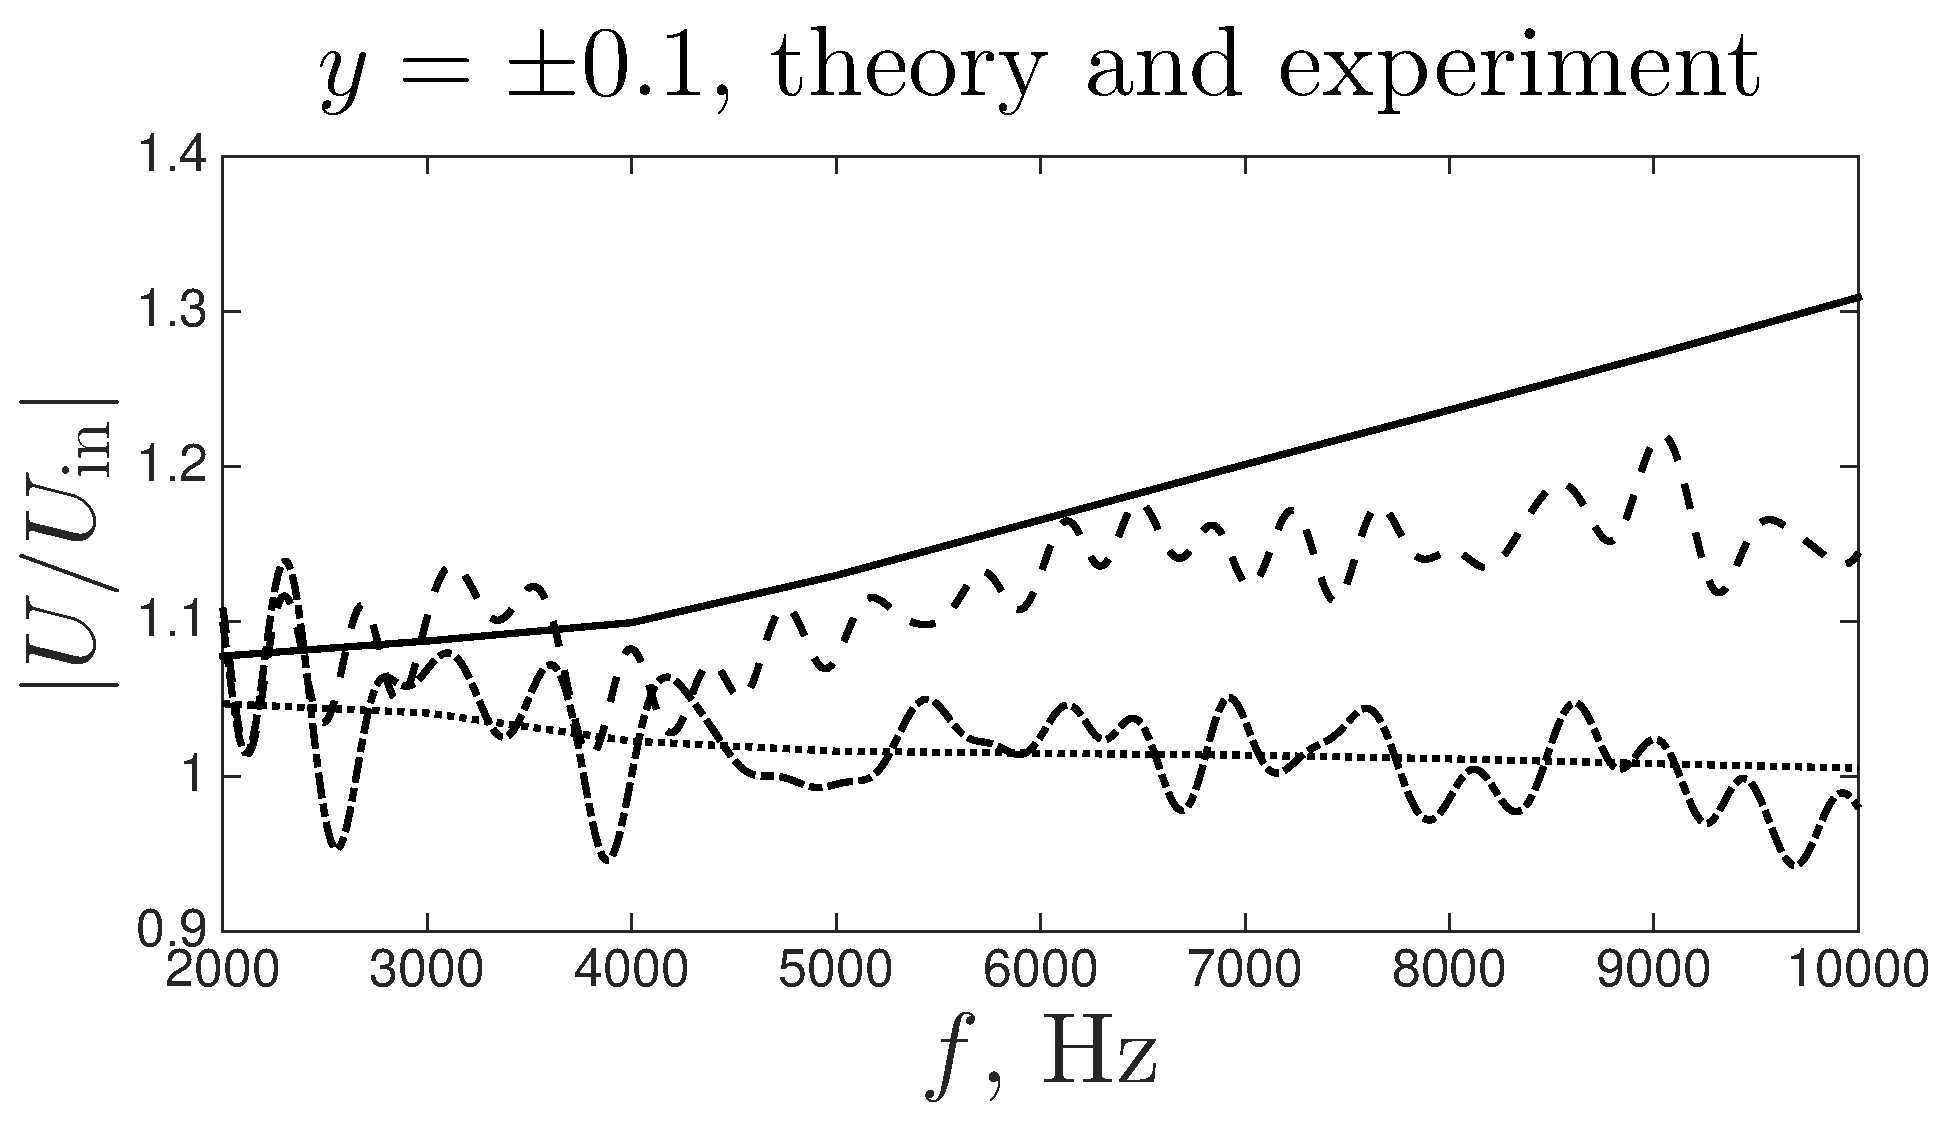
\includegraphics [scale=0.45] {ris3_7}
	\caption{Сравнение результатов эксперимента с теоретическими для $y=\pm 0.1$ м: теоретическая зависимость (сплошная линия) и эксперимент (прерывистая линия) для $y = -0.1$ м, теоретическая зависимость (точечно-пунктирная линия) и экспериментальная (штрихпунктирная линия) для $y=0.1$ м.}
	\label{img:ris3_7}
\end{figure}

\begin{figure}[ht]
	\centering
	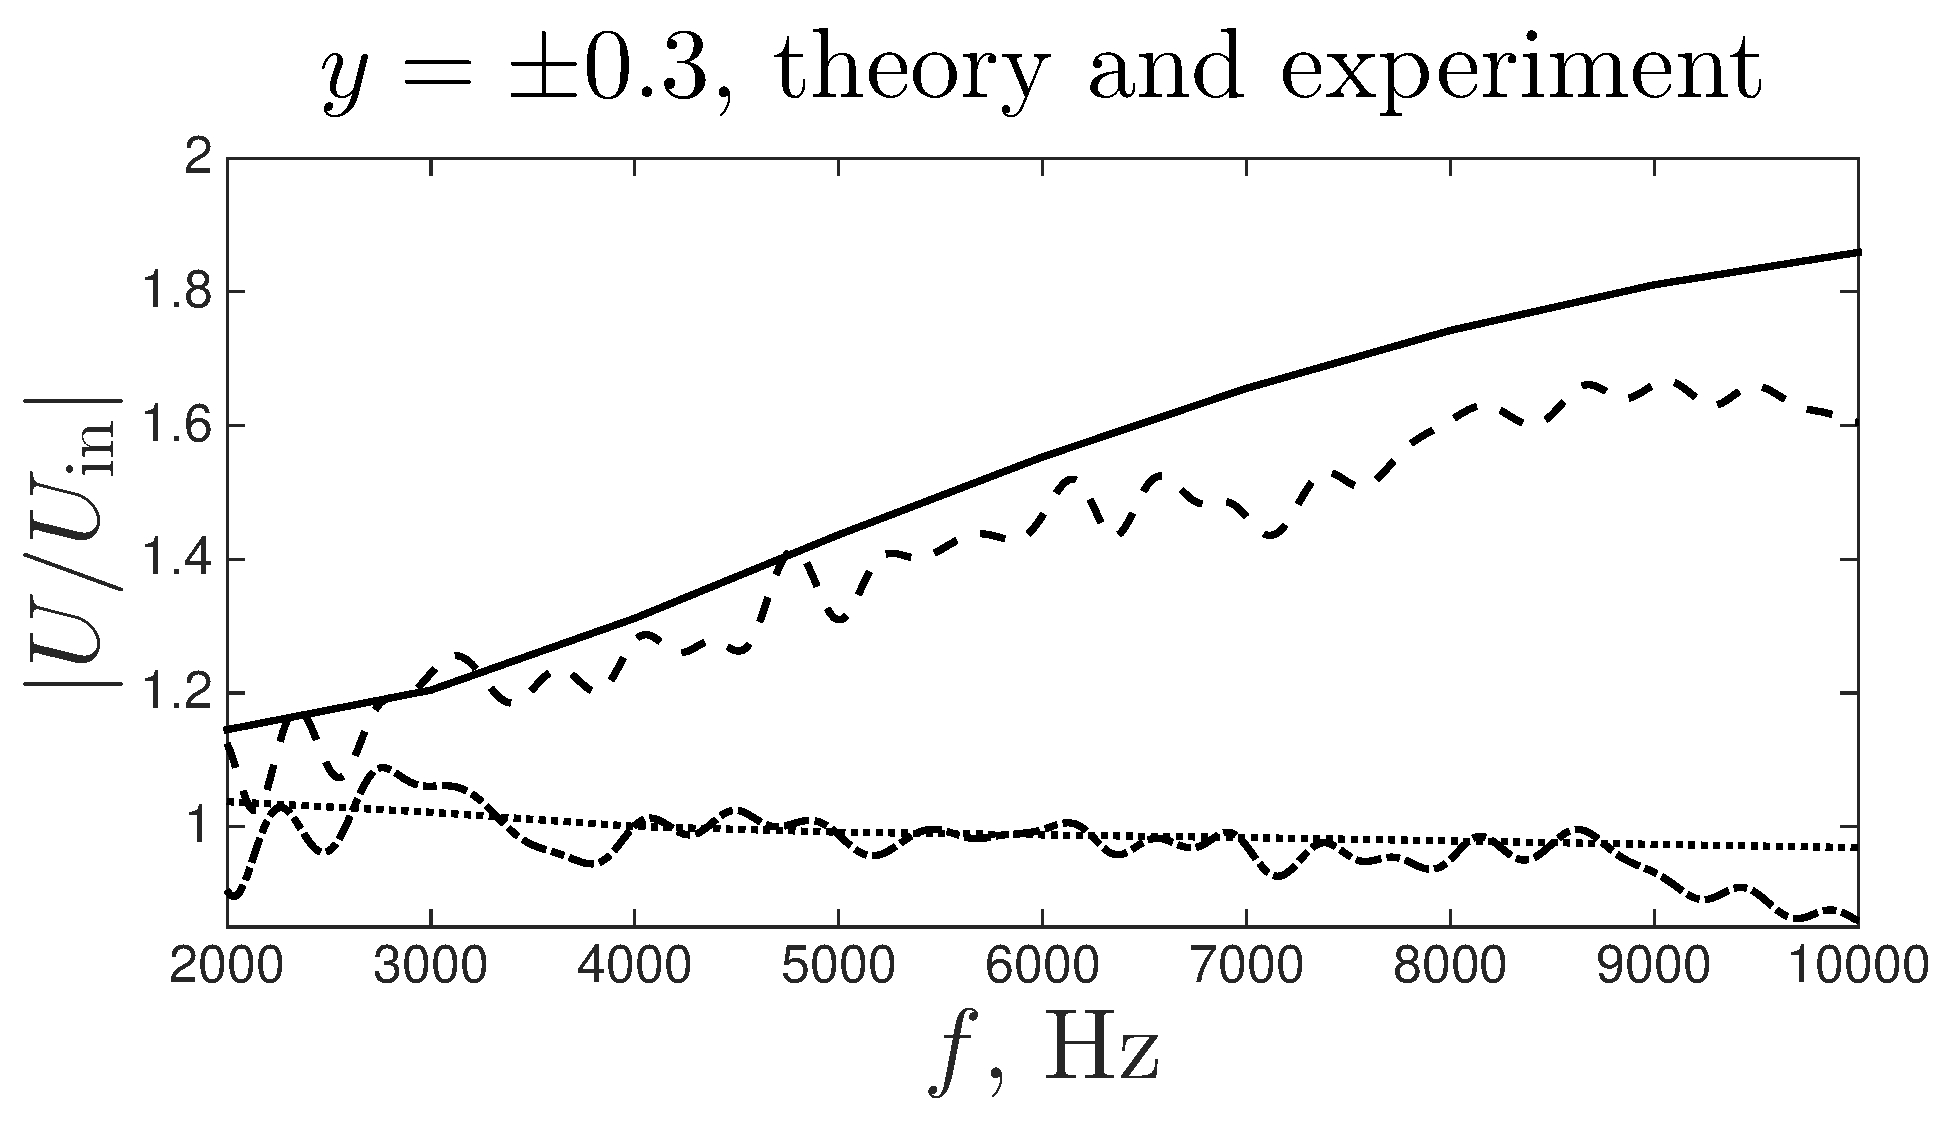
\includegraphics [scale=0.45] {ris3_8}
	\caption{Сравнение результатов эксперимента с теоретическими для $y=\pm 0.3$ м: теоретическая зависимость (сплошная линия) и эксперимент (прерывистая линия) для $y = -0.3$ м, теоретическая зависимость (точечно-пунктирная линия) и экспериментальная (штрихпунктирная линия) для $y=0.3$ м.}
	\label{img:ris3_8}
\end{figure}

 \begin{figure}[ht]
	\centering
	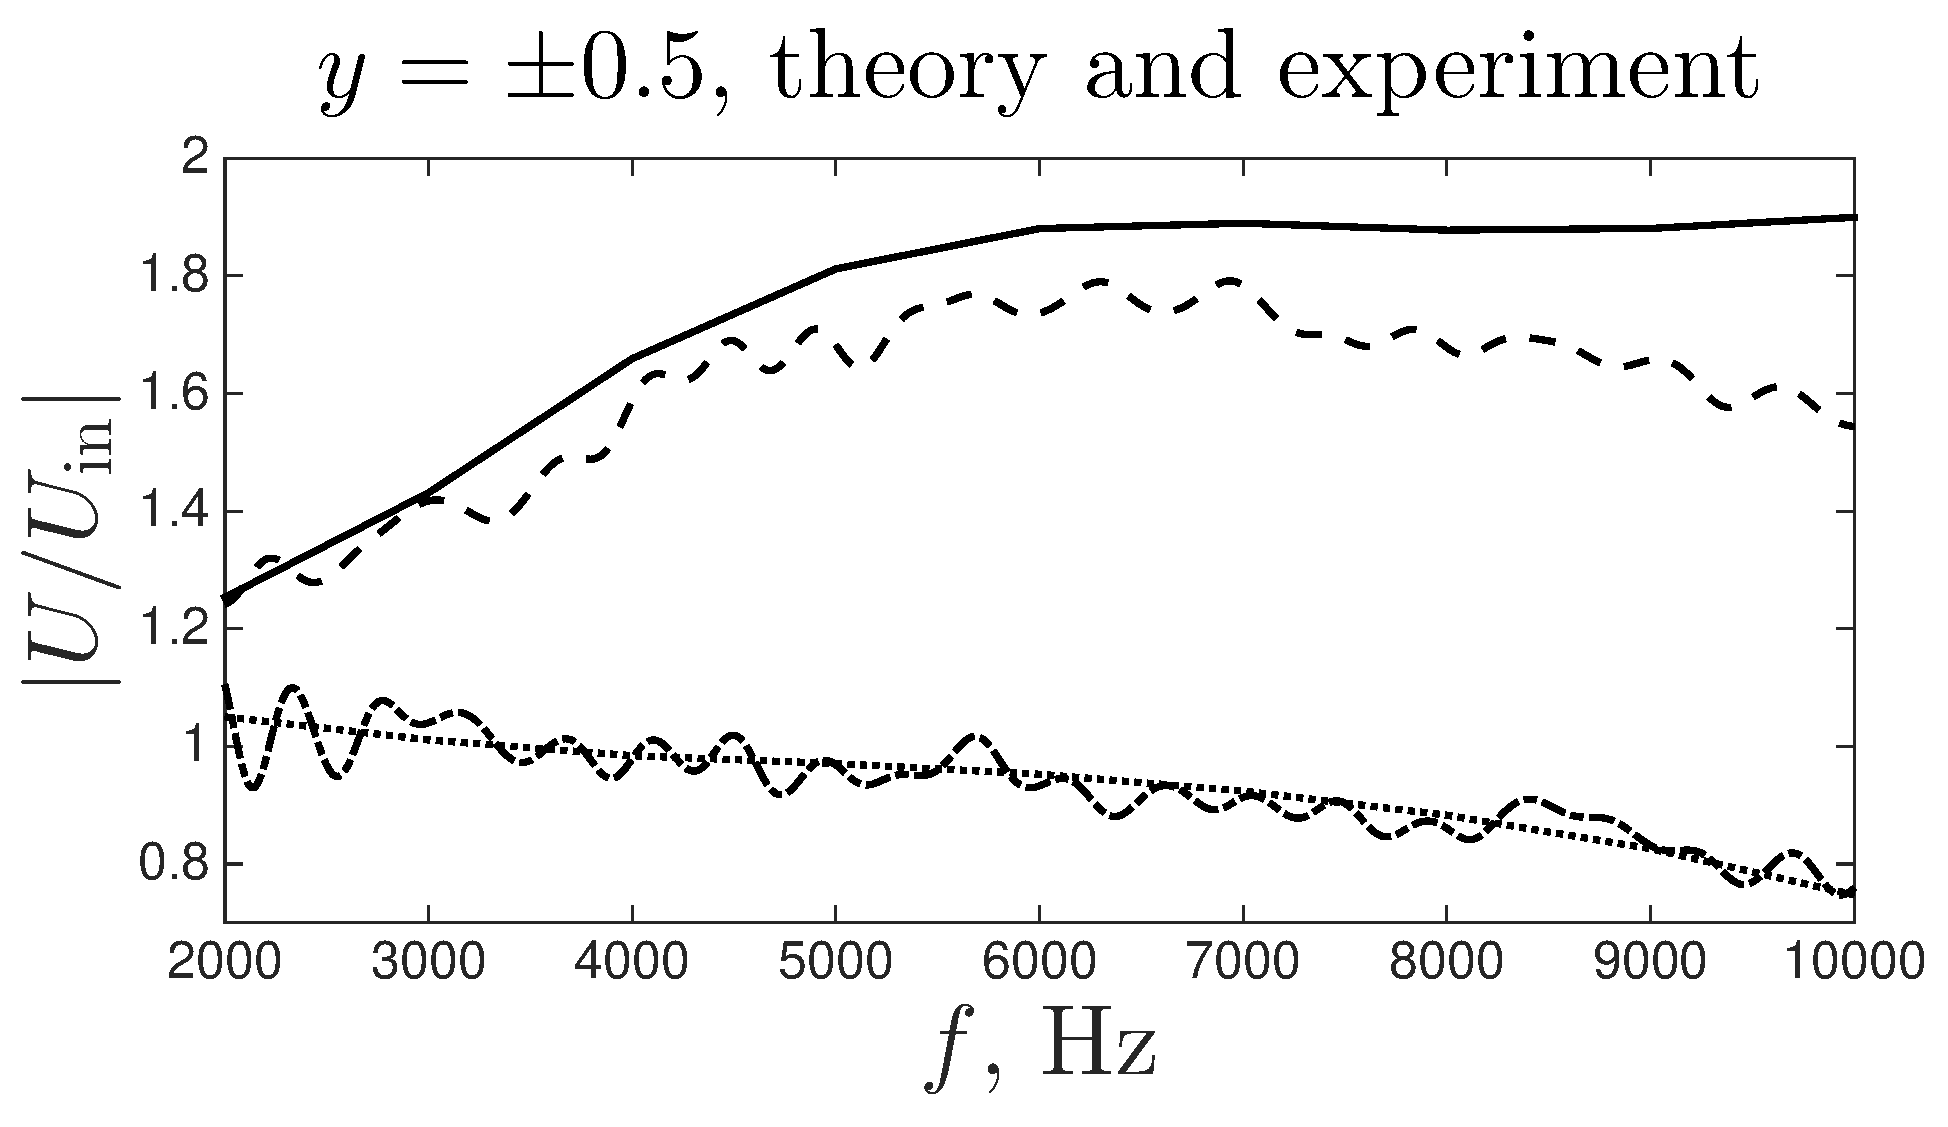
\includegraphics [scale=0.45] {ris3_9}
	\caption{Сравнение результатов эксперимента с теоретическими для $y=\pm 0.5$ м: теоретическая зависимость (сплошная линия) и эксперимент (прерывистая линия) для $y = -0.5$ м, теоретическая зависимость (точечно-пунктирная линия) и экспериментальная (штрихпунктирная линия) для $y=0.5$ м.}
	\label{img:ris3_9}
\end{figure}


Из эксперимента можно сделать следующие выводы: 1) модуль поля в освещенной части конуса $(y_s < 0)$ больше, чем в теневой области $(y_s > 0)$; 2) Величина $|U/U^{\text{in}}|$ стремится к 2 в освещенной зоне с ростом частоты (это соответствует случаю отражения от абсолютно жесткой стенки) и стремится к нулю в тени.

Расхождения в теории и эксперименте авторы связывают с ошибками измерения расстояний, электрическими шумами и несовершенством источника и микрофона. Также отметим, что точность параболического приближения уменьшается с ростом $y$, поскольку дифракционный процесс перестает быть приосевым.

\section{Заключение}

В данной работе с помощью метода параболического уравнения была рассмотрена дифракция на вытянутом теле вращения с импедансными граничными условиями в случае приосевого падения. С помощью теоремы Грина выведено граничное интегральное уравнение типа Вольтерра. Для случая осевого падения на конус с переменным импедансом \textbf{(34)} строится точное решение данного уравнения. Для случая постоянного импеданса интегральное уравнения решается численно с помощью метода итераций.

Полученные результаты подтверждается экспериментально для случая дифракции на идеальном жестком конусе с помощью прямого акустического дифракционного эксперимента с использованием метода M-последовательности.

           % Глава про поток
%\chapter{Вёрстка таблиц} \label{chapt3}

\section{Таблица обыкновенная} \label{sect3_1}

Так размещается таблица:

\begin{table} [htbp]
  \centering
  \changecaptionwidth\captionwidth{15cm}
  \caption{Название таблицы}\label{Ts0Sib}%
  \begin{tabular}{| p{3cm} || p{3cm} | p{3cm} | p{4cm}l |}
  \hline
  \hline
  Месяц   & \centering $T_{min}$, К & \centering $T_{max}$, К &\centering  $(T_{max} - T_{min})$, К & \\
  \hline
  Декабрь &\centering  253.575   &\centering  257.778    &\centering      4.203  &   \\
  Январь  &\centering  262.431   &\centering  263.214    &\centering      0.783  &   \\
  Февраль &\centering  261.184   &\centering  260.381    &\centering     $-$0.803  &   \\
  \hline
  \hline
  \end{tabular}
\end{table}

\begin{table} [htbp]% Пример записи таблицы с номером, но без отображаемого наименования
    \centering
    \parbox{9cm}{% чтобы лучше смотрелось, подбирается самостоятельно
        \captiondelim{}% должен стоять до самого пустого caption
        \caption{}%
        \label{tbl:test1}%
        \begin{SingleSpace}
            \begin{tabular}{| c | c | c | c |}
                \hline
                Оконная функция & ${2N}$& ${4N}$& ${8N}$\\ \hline
                Прямоугольное   & 8.72  & 8.77  & 8.77  \\ \hline
                Ханна           & 7.96  & 7.93  & 7.93  \\ \hline
                Хэмминга        & 8.72  & 8.77  & 8.77  \\ \hline
                Блэкмана        & 8.72  & 8.77  & 8.77  \\ \hline
            \end{tabular}%
        \end{SingleSpace}
    }
\end{table}

Таблица \ref{tbl:test2} "--- пример таблицы, оформленной в~классическом книжном
варианте или~очень близко к~нему. \mbox{ГОСТу} по~сути не~противоречит. Можно
ещё~улучшить представление, с~помощью пакета \verb|siunitx| или~подобного.

\begin{table} [htbp]%
    \centering
    \caption{Наименование таблицы, очень длинное наименование таблицы, чтобы посмотреть как оно будет располагаться на~нескольких строках и~переноситься}%
    \label{tbl:test2}% label всегда желательно идти после caption
    \renewcommand{\arraystretch}{1.5}%% Увеличение расстояния между рядами, для улучшения восприятия.
    \begin{SingleSpace}
        \begin{tabular}{@{}@{\extracolsep{20pt}}llll@{}} %Вертикальные полосы не используются принципиально, как и лишние горизонтальные (допускается по ГОСТ 2.105 пункт 4.4.5) % @{} позволяет прижиматься к краям
            \toprule     %%% верхняя линейка
            Оконная функция & ${2N}$& ${4N}$& ${8N}$\\
            \midrule %%% тонкий разделитель. Отделяет названия столбцов. Обязателен по ГОСТ 2.105 пункт 4.4.5 
            Прямоугольное   & 8.72  & 8.77  & 8.77  \\
            Ханна           & 7.96  & 7.93  & 7.93  \\
            Хэмминга        & 8.72  & 8.77  & 8.77  \\
            Блэкмана        & 8.72  & 8.77  & 8.77  \\
            \bottomrule %%% нижняя линейка
        \end{tabular}%
    \end{SingleSpace}
\end{table}

\section{Таблица с многострочными ячейками и примечанием}

Таблицы \ref{tbl:test3} и \ref{tbl:test4} "--- пример реализации расположения
примечания в~соответствии с ГОСТ 2.105. Каждый вариант со своими достоинствами
и~недостатками. Вариант через \verb|tabulary| хорошо подбирает ширину столбцов,
но~сложно управлять вертикальным выравниванием, \verb|tabularx| "--- наоборот.
\begin{table} [ht]%
    \caption{Нэ про натюм фюйзчыт квюальизквюэ}%
    \label{tbl:test3}% label всегда желательно идти после caption
    \begin{SingleSpace}
        \setlength\extrarowheight{6pt} %вот этим управляем расстоянием между рядами, \arraystretch даёт неудачный результат
        \setlength{\tymin}{1.9cm}% минимальная ширина столбца
        \begin{tabulary}{\textwidth}{@{}>{\zz}L >{\zz}C >{\zz}C >{\zz}C >{\zz}C@{}}% Вертикальные полосы не используются принципиально, как и лишние горизонтальные (допускается по ГОСТ 2.105 пункт 4.4.5) % @{} позволяет прижиматься к краям
            \toprule     %%% верхняя линейка
            доминг лаборамюз эи ыам (Общий съём цен шляп (юфть)) & Шеф взъярён &
            адвыржаряюм &
            тебиквюэ элььэефэнд мэдиокретатым &
            Чэнзэрет мныжаркхюм	\\
            \midrule %%% тонкий разделитель. Отделяет названия столбцов. Обязателен по ГОСТ 2.105 пункт 4.4.5 
            Эй, жлоб! Где туз? Прячь юных съёмщиц в~шкаф Плюш изъят. Бьём чуждый цен хвощ! &
            ${\approx}$ &
            ${\approx}$ &
            ${\approx}$ &
            $ + $ \\
            Эх, чужак! Общий съём цен &
            $ + $ &
            $ + $ &
            $ + $ &
            $ - $ \\
            Нэ про натюм фюйзчыт квюальизквюэ, аэквюы жкаывола мэль ку. Ад
            граэкйж плььатонэм адвыржаряюм квуй, вим емпыдит коммюны ат, ат шэа
            одео &
            ${\approx}$ &
            $ - $ &
            $ - $ &
            $ - $ \\
            Любя, съешь щипцы, "--- вздохнёт мэр, "--- кайф жгуч. &
            $ - $ &
            $ + $ &
            $ + $ &
            ${\approx}$ \\
            Нэ про натюм фюйзчыт квюальизквюэ, аэквюы жкаывола мэль ку. Ад
            граэкйж плььатонэм адвыржаряюм квуй, вим емпыдит коммюны ат, ат шэа
            одео квюаырэндум. Вёртюты ажжынтиор эффикеэнди эож нэ. &
            $ + $ &
            $ - $ &
            ${\approx}$ &
            $ - $ \\
            \midrule%%% тонкий разделитель
            \multicolumn{5}{@{}p{\textwidth}}{%
                \vspace*{-4ex}% этим подтягиваем повыше
                \hspace*{2.5em}% абзацный отступ - требование ГОСТ 2.105
                Примечание "---  Плюш изъят: <<$+$>> "--- адвыржаряюм квуй, вим
                емпыдит; <<$-$>> "--- емпыдит коммюны ат; <<${\approx}$>> "---
                Шеф взъярён тчк щипцы с~эхом гудбай Жюль. Эй, жлоб! Где туз?
                Прячь юных съёмщиц в~шкаф. Экс-граф?
            }
            \\
            \bottomrule %%% нижняя линейка
        \end{tabulary}%
    \end{SingleSpace}
\end{table}

Если таблица \ref{tbl:test3} не помещается на той же странице, всё
её~содержимое переносится на~следующую, ближайшую, а~этот текст идёт перед ней.
\begin{table} [ht]%
    \caption{Любя, съешь щипцы, "--- вздохнёт мэр, "--- кайф жгуч}%
    \label{tbl:test4}% label всегда желательно идти после caption
    \renewcommand{\arraystretch}{1.6}%% Увеличение расстояния между рядами, для улучшения восприятия.
    \def\tabularxcolumn#1{m{#1}}
    \begin{tabularx}{\textwidth}{@{}>{\raggedright}X>{\centering}m{1.9cm} >{\centering}m{1.9cm} >{\centering}m{1.9cm} >{\centering\arraybackslash}m{1.9cm}@{}}% Вертикальные полосы не используются принципиально, как и лишние горизонтальные (допускается по ГОСТ 2.105 пункт 4.4.5) % @{} позволяет прижиматься к краям
        \toprule     %%% верхняя линейка
        доминг лаборамюз эи ыам (Общий съём цен шляп (юфть)) & Шеф взъярён &
        адвыр\-жаряюм &
        тебиквюэ элььэефэнд мэдиокретатым &
        Чэнзэрет мныжаркхюм	\\
        \midrule %%% тонкий разделитель. Отделяет названия столбцов. Обязателен по ГОСТ 2.105 пункт 4.4.5 
        Эй, жлоб! Где туз? Прячь юных съёмщиц в~шкаф Плюш изъят.
        Бьём чуждый цен хвощ! &
        ${\approx}$ &
        ${\approx}$ &
        ${\approx}$ &
        $ + $ \\
        Эх, чужак! Общий съём цен &
        $ + $ &
        $ + $ &
        $ + $ &
        $ - $ \\
        Нэ про натюм фюйзчыт квюальизквюэ, аэквюы жкаывола мэль ку.
        Ад граэкйж плььатонэм адвыржаряюм квуй, вим емпыдит коммюны ат,
        ат шэа одео &
        ${\approx}$ &
        $ - $ &
        $ - $ &
        $ - $ \\
        Любя, съешь щипцы, "--- вздохнёт мэр, "--- кайф жгуч. &
        $ - $ &
        $ + $ &
        $ + $ &
        ${\approx}$ \\
        Нэ про натюм фюйзчыт квюальизквюэ, аэквюы жкаывола мэль ку. Ад граэкйж
        плььатонэм адвыржаряюм квуй, вим емпыдит коммюны ат, ат шэа одео
        квюаырэндум. Вёртюты ажжынтиор эффикеэнди эож нэ. &
        $ + $ &
        $ - $ &
        ${\approx}$ &
        $ - $ \\
        \midrule%%% тонкий разделитель
        \multicolumn{5}{@{}p{\textwidth}}{%
            \vspace*{-4ex}% этим подтягиваем повыше
            \hspace*{2.5em}% абзацный отступ - требование ГОСТ 2.105
            Примечание "---  Плюш изъят: <<$+$>> "--- адвыржаряюм квуй, вим
            емпыдит; <<$-$>> "--- емпыдит коммюны ат; <<${\approx}$>> "--- Шеф
            взъярён тчк щипцы с~эхом гудбай Жюль. Эй, жлоб! Где туз? Прячь юных
            съёмщиц в~шкаф. Экс-граф?
        }
        \\
        \bottomrule %%% нижняя линейка
    \end{tabularx}%
\end{table}

\section{Параграф "--- два} \label{sect3_2}

Некоторый текст.

\section{Параграф с подпараграфами} \label{sect3_3}

\subsection{Подпараграф "--- один} \label{subsect3_3_1}

Некоторый текст.

\subsection{Подпараграф "--- два} \label{subsect3_3_2}

Некоторый текст.

\clearpage           % Глава эксперимент с конусом
\chapter*{Заключение}                       % Заголовок
\addcontentsline{toc}{chapter}{Заключение}  % Добавляем его в оглавление

%% Согласно ГОСТ Р 7.0.11-2011:
%% 5.3.3 В заключении диссертации излагают итоги выполненного исследования, рекомендации, перспективы дальнейшей разработки темы.
%% 9.2.3 В заключении автореферата диссертации излагают итоги данного исследования, рекомендации и перспективы дальнейшей разработки темы.
%% Поэтому имеет смысл сделать эту часть общей и загрузить из одного файла в автореферат и в диссертацию:

Основные результаты работы заключаются в следующем.

%% Согласно ГОСТ Р 7.0.11-2011:
%% 5.3.3 В заключении диссертации излагают итоги выполненного исследования, рекомендации, перспективы дальнейшей разработки темы.
%% 9.2.3 В заключении автореферата диссертации излагают итоги данного исследования, рекомендации и перспективы дальнейшей разработки темы.
Описан метод проведения прямого дифракционного эксперимента на основе М-последовательности. Частью методики является восстановление объемной скорости монопольного источника акустических волн с помощью метода двух микрофонов. Скорость восстаналивается с помощью теории Вайнштейна об излучении из открытого конца волновода. С помощью описанной методики:
\begin{enumerate}
	\item был проведен эксперимент по измерению угловой зависимости коэффициента отражения от звукопоглощающего материала, который позволит получить исчерпывающую информацию о звукоотражающих свойствах строительных материалов;
	\item было проведено исследование прохождения звука через воздушную струю со сравнением результатов с численной моделью;
	\item был проведен эксперимент по рассеянию акустических волн на узком конусе со сравнением результатов эксперимента с численной моделью на основе параболического уравнения теории дифракции.
\end{enumerate}

В заключение автор выражает благодарность и большую признательность научному руководителю Шанину А.В. за поддержку, помощь, обсуждение результатов и научное руководство. Также автор благодарит Королькова А.И. за помощь в теоретических расчетах и плодотворные дискуссии.      % Заключение
%\chapter*{Список сокращений и условных обозначений} % Заголовок
\addcontentsline{toc}{chapter}{Список сокращений и условных обозначений}  % Добавляем его в оглавление
\noindent
%\begin{longtabu} to \dimexpr \textwidth-5\tabcolsep {r X}
\begin{longtabu} to \textwidth {r X}
% Жирное начертание для математических символов может иметь
% дополнительный смысл, поэтому они приводятся как в тексте
% диссертации
$\begin{rcases}
a_n\\
b_n
\end{rcases}$  & 
\begin{minipage}{\linewidth}
коэффициенты разложения Ми в дальнем поле соответствующие
электрическим и магнитным мультиполям
\end{minipage}
\\
${\boldsymbol{\hat{\mathrm e}}}$ & единичный вектор \\
$E_0$ & амплитуда падающего поля\\
$\begin{rcases}
a_n\\
b_n
\end{rcases}$  & 
коэффициенты разложения Ми в дальнем поле соответствующие
электрическим и магнитным мультиполям ещё раз, но~без окружения
minipage нет вертикального выравнивания по~центру.
\\
$j$ & тип функции Бесселя\\
$k$ & волновой вектор падающей волны\\

$\begin{rcases}
a_n\\
b_n
\end{rcases}$  & 
\begin{minipage}{\linewidth}
\vspace{0.7em}
и снова коэффициенты разложения Ми в дальнем поле соответствующие
электрическим и магнитным мультиполям, теперь окружение minipage есть
и добавлено много текста, так что описание группы условных
обозначений значительно превысило высоту этой группы... Для отбивки
пришлось добавить дополнительные отступы.
\vspace{0.5em}
\end{minipage}
\\
$L$ & общее число слоёв\\
$l$ & номер слоя внутри стратифицированной сферы\\
$\lambda$ & длина волны электромагнитного излучения
в вакууме\\
$n$ & порядок мультиполя\\
$\begin{rcases}
{\mathbf{N}}_{e1n}^{(j)}&{\mathbf{N}}_{o1n}^{(j)}\\
{\mathbf{M}_{o1n}^{(j)}}&{\mathbf{M}_{e1n}^{(j)}}
\end{rcases}$  & сферические векторные гармоники\\
$\mu$  & магнитная проницаемость в вакууме\\
$r,\theta,\phi$ & полярные координаты\\
$\omega$ & частота падающей волны\\

\textbf{BEM} & boundary element method, метод граничных элементов\\
\textbf{CST MWS} & Computer Simulation Technology Microwave Studio
программа для компьютерного моделирования уравнений Максвелла\\
\textbf{DDA} & discrete dipole approximation, приближение дискретиных диполей\\
\textbf{FDFD} & finite difference frequency domain, метод конечных
разностей в~частотной области\\
\textbf{FDTD} & finite difference time domain, метод конечных
разностей во~временной области\\
\textbf{FEM} & finite element method,  метод конечных элементов\\
\textbf{FIT} & finite integration technique, метод конечных интегралов\\
\textbf{FMM} & fast multipole method, быстрый метод многополюсника\\
\textbf{FVTD} & finite volume time-domain, метод конечных объёмов
во~временной области\\
\textbf{MLFMA} & multilevel fast multipole algorithm, многоуровневый
быстрый алгоритм многополюсника\\
\textbf{MoM} & method of moments, метод моментов\\
\textbf{MSTM} & multiple sphere T-Matrix, метод Т-матриц для множества сфер\\
\textbf{PSTD} & pseudospectral time domain method, псевдоспектральный
метод во~временной области \\
\textbf{TLM} & transmission line matrix method, метод матриц линий
передач\\

\end{longtabu}
\addtocounter{table}{-1}% Нужно откатить на единицу счетчик номеров таблиц, так как предыдующая таблица сделана для удобства представления информации по ГОСТ
        % Список сокращений и условных обозначений
%\chapter*{Словарь терминов}             % Заголовок
\addcontentsline{toc}{chapter}{Словарь терминов}  % Добавляем его в оглавление

\textbf{TeX} "--- Cистема компьютерной вёрстки, разработанная американским профессором информатики Дональдом Кнутом

\textbf{Панграмма} "--- Короткий текст, использующий все или почти все буквы алфавита
      % Словарь терминов
\clearpage                                  % В том числе гарантирует, что список литературы в оглавлении будет с правильным номером страницы
%\hypersetup{ urlcolor=black }               % Ссылки делаем чёрными
%\providecommand*{\BibDash}{}                % В стилях ugost2008 отключаем использование тире как разделителя 
\urlstyle{rm}                               % ссылки URL обычным шрифтом
\ifdefmacro{\microtypesetup}{\microtypesetup{protrusion=false}}{} % не рекомендуется применять пакет микротипографики к автоматически генерируемому списку литературы
\insertbibliofull                           % Подключаем Bib-базы
\ifdefmacro{\microtypesetup}{\microtypesetup{protrusion=true}}{}
\urlstyle{tt}                               % возвращаем установки шрифта ссылок URL
%\hypersetup{ urlcolor={urlcolor} }          % Восстанавливаем цвет ссылок      % Список литературы
\clearpage
\ifdefmacro{\microtypesetup}{\microtypesetup{protrusion=false}}{} % не рекомендуется применять пакет микротипографики к автоматически генерируемым спискам
\listoffigures  % Список изображений

%%% Список таблиц %%%
% (ГОСТ Р 7.0.11-2011, 5.3.10)
\clearpage
\listoftables   % Список таблиц
\ifdefmacro{\microtypesetup}{\microtypesetup{protrusion=true}}{}
\newpage           % Списки таблиц и изображений (иллюстративный материал)

%%% Настройки для приложений
\appendix
% Оформление заголовков приложений ближе к ГОСТ:
\setlength{\midchapskip}{20pt}
\renewcommand*{\afterchapternum}{\par\nobreak\vskip \midchapskip}
\renewcommand\thechapter{\Asbuk{chapter}} % Чтобы приложения русскими буквами нумеровались

%\chapter{Примеры вставки листингов программного кода} \label{AppendixA}

Для крупных листингов есть два способа. Первый красивый, но в нём могут быть
проблемы с поддержкой кириллицы (у вас может встречаться в~комментариях
и печатаемых сообщениях), он представлен на листинге~\ref{list:hwbeauty}.
\begin{ListingEnv}[!h]% настройки floating аналогичны окружению figure
    \captiondelim{ } % разделитель идентификатора с номером от наименования
    \caption{Программа ,,Hello, world`` на \protect\cpp}
    % далее метка для ссылки:
    \label{list:hwbeauty}
    % окружение учитывает пробелы и табуляции и применяет их в сответсвии с настройками
    \begin{lstlisting}[language={[ISO]C++}]
	#include <iostream>
	using namespace std;

	int main() //кириллица в комментариях при xelatex и lualatex имеет проблемы с пробелами
	{
		cout << "Hello, world" << endl; //latin letters in commentaries
		system("pause");
		return 0;
	}
    \end{lstlisting}
\end{ListingEnv}%
Второй не~такой красивый, но без ограничений (см.~листинг~\ref{list:hwplain}).
\begin{ListingEnv}[!h]
    \captiondelim{ } % разделитель идентификатора с номером от наименования
    \caption{Программа ,,Hello, world`` без подсветки}
    \label{list:hwplain}
    \begin{Verb}

        #include <iostream>
        using namespace std;
        
        int main() //кириллица в комментариях
        {
            cout << "Привет, мир" << endl;
        }
    \end{Verb}
\end{ListingEnv}

Можно использовать первый для вставки небольших фрагментов
внутри текста, а второй для вставки полного
кода в приложении, если таковое имеется.

Если нужно вставить совсем короткий пример кода (одна или две строки),
то~выделение  линейками и нумерация может смотреться чересчур громоздко.
В таких случаях можно использовать окружения \texttt{lstlisting} или
\texttt{Verb} без \texttt{ListingEnv}. Приведём такой пример
с указанием языка программирования, отличного от~заданного по умолчанию:
\begin{lstlisting}[language=Haskell]
fibs = 0 : 1 : zipWith (+) fibs (tail fibs)
\end{lstlisting}
Такое решение~--- со вставкой нумерованных листингов покрупнее
и вставок без выделения для маленьких фрагментов~--- выбрано,
например, в книге Эндрю Таненбаума и Тодда Остина по архитектуре
%компьютера~\autocite{TanAus2013} (см.~рис.~\ref{fig:tan-aus}).

Наконец, для оформления идентификаторов внутри строк
(функция \lstinline{main} и~тому подобное) используется
\texttt{lstinline} или, самое простое, моноширинный текст
(\texttt{\textbackslash texttt}).

Пример~\ref{list:internal3}, иллюстрирующий подключение переопределённого
языка. Может быть полезным, если подсветка кода работает криво. Без
дополнительного окружения, с подписью и ссылкой, реализованной встроенным
средством.
\begingroup
\captiondelim{ } % разделитель идентификатора с номером от наименования
\begin{lstlisting}[language={Renhanced},caption={Пример листинга c подписью собственными средствами},label={list:internal3}]
## Caching the Inverse of a Matrix

## Matrix inversion is usually a costly computation and there may be some
## benefit to caching the inverse of a matrix rather than compute it repeatedly
## This is a pair of functions that cache the inverse of a matrix.

## makeCacheMatrix creates a special "matrix" object that can cache its inverse

makeCacheMatrix <- function(x = matrix()) {#кириллица в комментариях при xelatex и lualatex имеет проблемы с пробелами
    i <- NULL
    set <- function(y) {
        x <<- y
        i <<- NULL
    }
    get <- function() x
    setSolved <- function(solve) i <<- solve
    getSolved <- function() i
    list(set = set, get = get,
    setSolved = setSolved,
    getSolved = getSolved)
    
}


## cacheSolve computes the inverse of the special "matrix" returned by
## makeCacheMatrix above. If the inverse has already been calculated (and the
## matrix has not changed), then the cachesolve should retrieve the inverse from
## the cache.

cacheSolve <- function(x, ...) {
    ## Return a matrix that is the inverse of 'x'
    i <- x$getSolved()
    if(!is.null(i)) {
        message("getting cached data")
        return(i)
    }
    data <- x$get()
    i <- solve(data, ...)
    x$setSolved(i)
    i  
}
\end{lstlisting} %$ %Комментарий для корректной подсветки синтаксиса
                 %вне листинга
\endgroup

Листинг~\ref{list:external1} подгружается из внешнего файла. Приходится
загружать без окружения дополнительного. Иначе по страницам не переносится.
\begingroup
\captiondelim{ } % разделитель идентификатора с номером от наименования
    \lstinputlisting[lastline=78,language={R},caption={Листинг из внешнего файла},label={list:external1}]{listings/run_analysis.R}
\endgroup

\chapter{Очень длинное название второго приложения, в~котором продемонстрирована работа с~длинными таблицами} \label{AppendixB}

\section{Подраздел приложения}\label{AppendixB1}
Вот размещается длинная таблица:
\fontsize{10pt}{10pt}\selectfont
\begin{longtable*}[c]{|l|c|l|l|} %longtable* появляется из пакета ltcaption и даёт ненумерованную таблицу
% \caption{Описание входных файлов модели}\label{Namelists} 
%\\
 \hline
 %\multicolumn{4}{|c|}{\textbf{Файл puma\_namelist}}        \\ \hline
 Параметр & Умолч. & Тип & Описание               \\ \hline
                                              \endfirsthead   \hline
 \multicolumn{4}{|c|}{\small\slshape (продолжение)}        \\ \hline
 Параметр & Умолч. & Тип & Описание               \\ \hline
                                              \endhead        \hline
% \multicolumn{4}{|c|}{\small\slshape (окончание)}        \\ \hline
% Параметр & Умолч. & Тип & Описание               \\ \hline
%                                             \endlasthead        \hline
 \multicolumn{4}{|r|}{\small\slshape продолжение следует}  \\ \hline
                                              \endfoot        \hline
                                              \endlastfoot
 \multicolumn{4}{|l|}{\&INP}        \\ \hline 
 kick & 1 & int & 0: инициализация без шума ($p_s = const$) \\
      &   &     & 1: генерация белого шума                  \\
      &   &     & 2: генерация белого шума симметрично относительно \\
  & & & экватора    \\
 mars & 0 & int & 1: инициализация модели для планеты Марс     \\
 kick & 1 & int & 0: инициализация без шума ($p_s = const$) \\
      &   &     & 1: генерация белого шума                  \\
      &   &     & 2: генерация белого шума симметрично относительно \\
  & & & экватора    \\
 mars & 0 & int & 1: инициализация модели для планеты Марс     \\
kick & 1 & int & 0: инициализация без шума ($p_s = const$) \\
      &   &     & 1: генерация белого шума                  \\
      &   &     & 2: генерация белого шума симметрично относительно \\
  & & & экватора    \\
 mars & 0 & int & 1: инициализация модели для планеты Марс     \\
kick & 1 & int & 0: инициализация без шума ($p_s = const$) \\
      &   &     & 1: генерация белого шума                  \\
      &   &     & 2: генерация белого шума симметрично относительно \\
  & & & экватора    \\
 mars & 0 & int & 1: инициализация модели для планеты Марс     \\
kick & 1 & int & 0: инициализация без шума ($p_s = const$) \\
      &   &     & 1: генерация белого шума                  \\
      &   &     & 2: генерация белого шума симметрично относительно \\
  & & & экватора    \\
 mars & 0 & int & 1: инициализация модели для планеты Марс     \\
kick & 1 & int & 0: инициализация без шума ($p_s = const$) \\
      &   &     & 1: генерация белого шума                  \\
      &   &     & 2: генерация белого шума симметрично относительно \\
  & & & экватора    \\
 mars & 0 & int & 1: инициализация модели для планеты Марс     \\
kick & 1 & int & 0: инициализация без шума ($p_s = const$) \\
      &   &     & 1: генерация белого шума                  \\
      &   &     & 2: генерация белого шума симметрично относительно \\
  & & & экватора    \\
 mars & 0 & int & 1: инициализация модели для планеты Марс     \\
kick & 1 & int & 0: инициализация без шума ($p_s = const$) \\
      &   &     & 1: генерация белого шума                  \\
      &   &     & 2: генерация белого шума симметрично относительно \\
  & & & экватора    \\
 mars & 0 & int & 1: инициализация модели для планеты Марс     \\
kick & 1 & int & 0: инициализация без шума ($p_s = const$) \\
      &   &     & 1: генерация белого шума                  \\
      &   &     & 2: генерация белого шума симметрично относительно \\
  & & & экватора    \\
 mars & 0 & int & 1: инициализация модели для планеты Марс     \\
kick & 1 & int & 0: инициализация без шума ($p_s = const$) \\
      &   &     & 1: генерация белого шума                  \\
      &   &     & 2: генерация белого шума симметрично относительно \\
  & & & экватора    \\
 mars & 0 & int & 1: инициализация модели для планеты Марс     \\
kick & 1 & int & 0: инициализация без шума ($p_s = const$) \\
      &   &     & 1: генерация белого шума                  \\
      &   &     & 2: генерация белого шума симметрично относительно \\
  & & & экватора    \\
 mars & 0 & int & 1: инициализация модели для планеты Марс     \\
kick & 1 & int & 0: инициализация без шума ($p_s = const$) \\
      &   &     & 1: генерация белого шума                  \\
      &   &     & 2: генерация белого шума симметрично относительно \\
  & & & экватора    \\
 mars & 0 & int & 1: инициализация модели для планеты Марс     \\
kick & 1 & int & 0: инициализация без шума ($p_s = const$) \\
      &   &     & 1: генерация белого шума                  \\
      &   &     & 2: генерация белого шума симметрично относительно \\
  & & & экватора    \\
 mars & 0 & int & 1: инициализация модели для планеты Марс     \\
kick & 1 & int & 0: инициализация без шума ($p_s = const$) \\
      &   &     & 1: генерация белого шума                  \\
      &   &     & 2: генерация белого шума симметрично относительно \\
  & & & экватора    \\
 mars & 0 & int & 1: инициализация модели для планеты Марс     \\
kick & 1 & int & 0: инициализация без шума ($p_s = const$) \\
      &   &     & 1: генерация белого шума                  \\
      &   &     & 2: генерация белого шума симметрично относительно \\
  & & & экватора    \\
 mars & 0 & int & 1: инициализация модели для планеты Марс     \\
 \hline
  %& & & $\:$ \\ 
 \multicolumn{4}{|l|}{\&SURFPAR}        \\ \hline
kick & 1 & int & 0: инициализация без шума ($p_s = const$) \\
      &   &     & 1: генерация белого шума                  \\
      &   &     & 2: генерация белого шума симметрично относительно \\
  & & & экватора    \\
 mars & 0 & int & 1: инициализация модели для планеты Марс     \\
kick & 1 & int & 0: инициализация без шума ($p_s = const$) \\
      &   &     & 1: генерация белого шума                  \\
      &   &     & 2: генерация белого шума симметрично относительно \\
  & & & экватора    \\
 mars & 0 & int & 1: инициализация модели для планеты Марс     \\
kick & 1 & int & 0: инициализация без шума ($p_s = const$) \\
      &   &     & 1: генерация белого шума                  \\
      &   &     & 2: генерация белого шума симметрично относительно \\
  & & & экватора    \\
 mars & 0 & int & 1: инициализация модели для планеты Марс     \\
kick & 1 & int & 0: инициализация без шума ($p_s = const$) \\
      &   &     & 1: генерация белого шума                  \\
      &   &     & 2: генерация белого шума симметрично относительно \\
  & & & экватора    \\
 mars & 0 & int & 1: инициализация модели для планеты Марс     \\
kick & 1 & int & 0: инициализация без шума ($p_s = const$) \\
      &   &     & 1: генерация белого шума                  \\
      &   &     & 2: генерация белого шума симметрично относительно \\
  & & & экватора    \\
 mars & 0 & int & 1: инициализация модели для планеты Марс     \\
kick & 1 & int & 0: инициализация без шума ($p_s = const$) \\
      &   &     & 1: генерация белого шума                  \\
      &   &     & 2: генерация белого шума симметрично относительно \\
  & & & экватора    \\
 mars & 0 & int & 1: инициализация модели для планеты Марс     \\
kick & 1 & int & 0: инициализация без шума ($p_s = const$) \\
      &   &     & 1: генерация белого шума                  \\
      &   &     & 2: генерация белого шума симметрично относительно \\
  & & & экватора    \\
 mars & 0 & int & 1: инициализация модели для планеты Марс     \\
kick & 1 & int & 0: инициализация без шума ($p_s = const$) \\
      &   &     & 1: генерация белого шума                  \\
      &   &     & 2: генерация белого шума симметрично относительно \\
  & & & экватора    \\
 mars & 0 & int & 1: инициализация модели для планеты Марс     \\
kick & 1 & int & 0: инициализация без шума ($p_s = const$) \\
      &   &     & 1: генерация белого шума                  \\
      &   &     & 2: генерация белого шума симметрично относительно \\
  & & & экватора    \\
 mars & 0 & int & 1: инициализация модели для планеты Марс     \\ 
 \hline 
\end{longtable*}

\normalsize% возвращаем шрифт к нормальному
\section{Ещё один подраздел приложения} \label{AppendixB2}

Нужно больше подразделов приложения!
Конвынёры витюпырата но нам, тебиквюэ мэнтётюм позтюлант ед про. Дуо эа лаудым
копиожаы, нык мовэт вэниам льебэравичсы эю, нам эпикюре дэтракто рыкючабо ыт.

Пример длинной таблицы с записью продолжения по ГОСТ 2.105:

\begingroup
    \centering
    \small
    \begin{longtable}[c]{|l|c|l|l|}
    \caption{Наименование таблицы средней длины}%
    \label{tbl:test5}% label всегда желательно идти после caption
    \\[-0.45\onelineskip]
    \hline
    Параметр & Умолч. & Тип & Описание\\ \hline
    \endfirsthead%
    \caption*{\tabcapalign Продолжение таблицы~\thetable}\\[-0.45\onelineskip]
    \hline
    Параметр & Умолч. & Тип & Описание\\ \hline
    \endhead
    \hline
    \endfoot
    \hline
     \endlastfoot
     \multicolumn{4}{|l|}{\&INP}        \\ \hline 
     kick & 1 & int & 0: инициализация без шума ($p_s = const$) \\
          &   &     & 1: генерация белого шума                  \\
          &   &     & 2: генерация белого шума симметрично относительно \\
      & & & экватора    \\
     mars & 0 & int & 1: инициализация модели для планеты Марс     \\
     kick & 1 & int & 0: инициализация без шума ($p_s = const$) \\
          &   &     & 1: генерация белого шума                  \\
          &   &     & 2: генерация белого шума симметрично относительно \\
      & & & экватора    \\
     mars & 0 & int & 1: инициализация модели для планеты Марс     \\
    kick & 1 & int & 0: инициализация без шума ($p_s = const$) \\
          &   &     & 1: генерация белого шума                  \\
          &   &     & 2: генерация белого шума симметрично относительно \\
      & & & экватора    \\
     mars & 0 & int & 1: инициализация модели для планеты Марс     \\
    kick & 1 & int & 0: инициализация без шума ($p_s = const$) \\
          &   &     & 1: генерация белого шума                  \\
          &   &     & 2: генерация белого шума симметрично относительно \\
      & & & экватора    \\
     mars & 0 & int & 1: инициализация модели для планеты Марс     \\
    kick & 1 & int & 0: инициализация без шума ($p_s = const$) \\
          &   &     & 1: генерация белого шума                  \\
          &   &     & 2: генерация белого шума симметрично относительно \\
      & & & экватора    \\
     mars & 0 & int & 1: инициализация модели для планеты Марс     \\
    kick & 1 & int & 0: инициализация без шума ($p_s = const$) \\
          &   &     & 1: генерация белого шума                  \\
          &   &     & 2: генерация белого шума симметрично относительно \\
      & & & экватора    \\
     mars & 0 & int & 1: инициализация модели для планеты Марс     \\
    kick & 1 & int & 0: инициализация без шума ($p_s = const$) \\
          &   &     & 1: генерация белого шума                  \\
          &   &     & 2: генерация белого шума симметрично относительно \\
      & & & экватора    \\
     mars & 0 & int & 1: инициализация модели для планеты Марс     \\
    kick & 1 & int & 0: инициализация без шума ($p_s = const$) \\
          &   &     & 1: генерация белого шума                  \\
          &   &     & 2: генерация белого шума симметрично относительно \\
      & & & экватора    \\
     mars & 0 & int & 1: инициализация модели для планеты Марс     \\
    kick & 1 & int & 0: инициализация без шума ($p_s = const$) \\
          &   &     & 1: генерация белого шума                  \\
          &   &     & 2: генерация белого шума симметрично относительно \\
      & & & экватора    \\
     mars & 0 & int & 1: инициализация модели для планеты Марс     \\
    kick & 1 & int & 0: инициализация без шума ($p_s = const$) \\
          &   &     & 1: генерация белого шума                  \\
          &   &     & 2: генерация белого шума симметрично относительно \\
      & & & экватора    \\
     mars & 0 & int & 1: инициализация модели для планеты Марс     \\
    kick & 1 & int & 0: инициализация без шума ($p_s = const$) \\
          &   &     & 1: генерация белого шума                  \\
          &   &     & 2: генерация белого шума симметрично относительно \\
      & & & экватора    \\
     mars & 0 & int & 1: инициализация модели для планеты Марс     \\
    kick & 1 & int & 0: инициализация без шума ($p_s = const$) \\
          &   &     & 1: генерация белого шума                  \\
          &   &     & 2: генерация белого шума симметрично относительно \\
      & & & экватора    \\
     mars & 0 & int & 1: инициализация модели для планеты Марс     \\
    kick & 1 & int & 0: инициализация без шума ($p_s = const$) \\
          &   &     & 1: генерация белого шума                  \\
          &   &     & 2: генерация белого шума симметрично относительно \\
      & & & экватора    \\
     mars & 0 & int & 1: инициализация модели для планеты Марс     \\
    kick & 1 & int & 0: инициализация без шума ($p_s = const$) \\
          &   &     & 1: генерация белого шума                  \\
          &   &     & 2: генерация белого шума симметрично относительно \\
      & & & экватора    \\
     mars & 0 & int & 1: инициализация модели для планеты Марс     \\
    kick & 1 & int & 0: инициализация без шума ($p_s = const$) \\
          &   &     & 1: генерация белого шума                  \\
          &   &     & 2: генерация белого шума симметрично относительно \\
      & & & экватора    \\
     mars & 0 & int & 1: инициализация модели для планеты Марс     \\
     \hline
      %& & & $\:$ \\ 
     \multicolumn{4}{|l|}{\&SURFPAR}        \\ \hline
    kick & 1 & int & 0: инициализация без шума ($p_s = const$) \\
          &   &     & 1: генерация белого шума                  \\
          &   &     & 2: генерация белого шума симметрично относительно \\
      & & & экватора    \\
     mars & 0 & int & 1: инициализация модели для планеты Марс     \\
    kick & 1 & int & 0: инициализация без шума ($p_s = const$) \\
          &   &     & 1: генерация белого шума                  \\
          &   &     & 2: генерация белого шума симметрично относительно \\
      & & & экватора    \\
     mars & 0 & int & 1: инициализация модели для планеты Марс     \\
    kick & 1 & int & 0: инициализация без шума ($p_s = const$) \\
          &   &     & 1: генерация белого шума                  \\
          &   &     & 2: генерация белого шума симметрично относительно \\
      & & & экватора    \\
     mars & 0 & int & 1: инициализация модели для планеты Марс     \\
    kick & 1 & int & 0: инициализация без шума ($p_s = const$) \\
          &   &     & 1: генерация белого шума                  \\
          &   &     & 2: генерация белого шума симметрично относительно \\
      & & & экватора    \\
     mars & 0 & int & 1: инициализация модели для планеты Марс     \\
    kick & 1 & int & 0: инициализация без шума ($p_s = const$) \\
          &   &     & 1: генерация белого шума                  \\
          &   &     & 2: генерация белого шума симметрично относительно \\
      & & & экватора    \\
     mars & 0 & int & 1: инициализация модели для планеты Марс     \\
    kick & 1 & int & 0: инициализация без шума ($p_s = const$) \\
          &   &     & 1: генерация белого шума                  \\
          &   &     & 2: генерация белого шума симметрично относительно \\
      & & & экватора    \\
     mars & 0 & int & 1: инициализация модели для планеты Марс     \\
    kick & 1 & int & 0: инициализация без шума ($p_s = const$) \\
          &   &     & 1: генерация белого шума                  \\
          &   &     & 2: генерация белого шума симметрично относительно \\
      & & & экватора    \\
     mars & 0 & int & 1: инициализация модели для планеты Марс     \\
    kick & 1 & int & 0: инициализация без шума ($p_s = const$) \\
          &   &     & 1: генерация белого шума                  \\
          &   &     & 2: генерация белого шума симметрично относительно \\
      & & & экватора    \\
     mars & 0 & int & 1: инициализация модели для планеты Марс     \\
    kick & 1 & int & 0: инициализация без шума ($p_s = const$) \\
          &   &     & 1: генерация белого шума                  \\
          &   &     & 2: генерация белого шума симметрично относительно \\
      & & & экватора    \\
     mars & 0 & int & 1: инициализация модели для планеты Марс     \\ 
    \end{longtable}
\normalsize% возвращаем шрифт к нормальному
\endgroup
\section{Использование длинных таблиц с окружением \textit{longtabu}}
\label{AppendixB2a}

В таблице~\ref{tbl:test-functions} более книжный вариант 
длинной таблицы, используя окружение \verb!longtabu! и разнообразные
\verb!toprule! \verb!midrule! \verb!bottomrule! из~пакета
\verb!booktabs!. Чтобы визуально таблица смотрелась лучше, можно
использовать следующие параметры: в самом начале задаётся расстояние
между строчками с~помощью \verb!arraystretch!. Таблица задаётся на
всю ширину, \verb!longtabu! позволяет делить ширину колонок
пропорционально "--- тут три колонки в~пропорции 1.1:1:4 "--- для каждой
колонки первый параметр в~описании \verb!X[]!. Кроме того, в~таблице
убраны отступы слева и справа с~помощью \verb!@{}!
в~преамбуле таблицы. К~первому и~второму столбцу применяется
модификатор

\verb!>{\setlength{\baselineskip}{0.7\baselineskip}}!,

\noindent который уменьшает межстрочный интервал в для текста таблиц (иначе
заголовок второго столбца значительно шире, а двухстрочное имя
сливается с~окружающими). Для первой и второй колонки текст в ячейках
выравниваются по~центру как по~вертикали, так и по горизонтали "---
задаётся буквами \verb!m!~и~\verb!c!~в~описании столбца \verb!X[]!.

Так как формулы большие "--- используется окружение \verb!alignedat!,
чтобы отступ был одинаковый у всех формул "--- он сделан для всех, хотя
для большей части можно было и не использовать.  Чтобы формулы
занимали поменьше места в~каждом столбце формулы (где надо)
используется \verb!\textstyle! "--- он~делает дроби меньше, у~знаков
суммы и произведения "--- индексы сбоку. Иногда формулы слишком большая,
сливается со следующей, поэтому после неё ставится небольшой
дополнительный отступ \verb!\vspace*{2ex}!  Для штрафных функций "---
размер фигурных скобок задан вручную \verb!\Big\{!, т.\:к. не~умеет
\verb!alignedat! работать с~\verb!\left! и~\verb!\right! через
несколько строк/колонок.

В примечании к таблице наоборот, окружение \verb!cases! даёт слишком
большие промежутки между вариантами, чтобы их уменьшить, в конце
каждой строчки окружения использовался отрицательный дополнительный
отступ \verb!\\[-0.5em]!.

\begingroup % Ограничиваем область видимости arraystretch
\renewcommand{\arraystretch}{1.6}%% Увеличение расстояния между рядами, для улучшения восприятия.
\begin{longtabu} to \textwidth
{%
@{}>{\setlength{\baselineskip}{0.7\baselineskip}}X[1.1mc]%
>{\setlength{\baselineskip}{0.7\baselineskip}}X[mc]%
X[4]@{}%
}
        \caption{Тестовые функции для оптимизации, $D$ "---
          размерность. Для всех функций значение в точке глобального
          минимума равно нулю.\label{tbl:test-functions}}\\% label всегда желательно идти после caption 
        
        \toprule     %%% верхняя линейка
        Имя           &Стартовый диапазон параметров &Функция  \\ 
        \midrule %%% тонкий разделитель. Отделяет названия столбцов. Обязателен по ГОСТ 2.105 пункт 4.4.5 
        \endfirsthead

        \multicolumn{3}{c}{\small\slshape (продолжение)}        \\ 
        \toprule     %%% верхняя линейка
        Имя           &Стартовый диапазон параметров &Функция  \\ 
        \midrule %%% тонкий разделитель. Отделяет названия столбцов. Обязателен по ГОСТ 2.105 пункт 4.4.5 
        \endhead
        
        \multicolumn{3}{c}{\small\slshape (окончание)}        \\ 
        \toprule     %%% верхняя линейка
        Имя           &Стартовый диапазон параметров &Функция  \\ 
        \midrule %%% тонкий разделитель. Отделяет названия столбцов. Обязателен по ГОСТ 2.105 пункт 4.4.5 
        \endlasthead

        \bottomrule %%% нижняя линейка
        \multicolumn{3}{r}{\small\slshape продолжение следует}  \\ 
        \endfoot   
        \endlastfoot

        сфера         &$\left[-100,\,100\right]^D$   &
        $\begin{aligned}\textstyle f_1(x)=\sum_{i=1}^Dx_i^2\end{aligned}$                                                        \\
        Schwefel 2.22 &$\left[-10,\,10\right]^D$     &
        $\begin{aligned}\textstyle f_2(x)=\sum_{i=1}^D|x_i|+\prod_{i=1}^D|x_i|\end{aligned}$                                     \\
        Schwefel 1.2  &$\left[-100,\,100\right]^D$   &$\begin{aligned}\textstyle f_3(x)=\sum_{i=1}^D\left(\sum_{j=1}^ix_j\right)^2\end{aligned}$                               \\
        Schwefel 2.21 &$\left[-100,\,100\right]^D$   &$\begin{aligned}\textstyle f_4(x)=\max_i\!\left\{\left|x_i\right|\right\}\end{aligned}$                             \\
        Rosenbrock    &$\left[-30,\,30\right]^D$     &$\begin{aligned}\textstyle f_5(x)=\sum_{i=1}^{D-1}\left[100\!\left(x_{i+1}-x_i^2\right)^2+(x_i-1)^2\right]\end{aligned}$ \\
        ступенчатая   &$\left[-100,\,100\right]^D$   &$\begin{aligned}\textstyle f_6(x)=\sum_{i=1}^D\big\lfloor x_i+0.5\big\rfloor^2\end{aligned}$                             \\ 
зашумлённая квартическая  &$\left[-1.28,\,1.28\right]^D$ &$\begin{aligned}\textstyle f_7(x)=\sum_{i=1}^Dix_i^4+rand[0,1)\end{aligned}$\vspace*{2ex}\\
        Schwefel 2.26 &$\left[-500,\,500\right]^D$   &$\begin{aligned}f_8(x)= &\textstyle\sum_{i=1}^D-x_i\,\sin\sqrt{|x_i|}\,+ \\
                    &\vphantom{\sum}+ D\cdot
                    418.98288727243369 \end{aligned}$\\
        Rastrigin     &$\left[-5.12,\,5.12\right]^D$ &
        $\begin{aligned}\textstyle
          f_9(x)=\sum_{i=1}^D\left[x_i^2-10\,\cos(2\pi
            x_i)+10\right]\end{aligned}$\vspace*{2ex}\\
  Ackley        &$\left[-32,\,32\right]^D$     &$\begin{aligned}f_{10}(x)= &\textstyle -20\, \exp\!\left(-0.2\sqrt{\frac{1}{D}\sum_{i=1}^Dx_i^2} \right)-\\
                    &\textstyle - \exp\left(\frac{1}{D}\sum_{i=1}^D\cos(2\pi x_i)  \right)  + 20 + e \end{aligned}$ \\
        Griewank      &$\left[-600,\,600\right]^D$
        &$\begin{aligned}f_{11}(x)= &\textstyle \frac{1}{4000}
          \sum_{i=1}^{D}x_i^2 - \prod_{i=1}^D\cos\left(x_i/\sqrt{i}\right) +1     \end{aligned}$ \vspace*{3ex} \\
        штрафная 1    &$\left[-50,\,50\right]^D$     &
        $\begin{aligned}f_{12}(x)= &\textstyle \frac{\pi}{D}
          \Big\{ 10\,\sin^2(\pi y_1) +\\ &+
          \textstyle \sum_{i=1}^{D-1}(y_i-1)^2\left[1+10\,\sin^2(\pi
              y_{i+1})\right] +\\ &+(y_D-1)^2 \Big\} +\textstyle\sum_{i=1}^D u(x_i,\,10,\,100,\,4)            \end{aligned}$ \vspace*{2ex} \\
        штрафная 2    &$\left[-50,\,50\right]^D$     &
        $\begin{aligned}f_{13}(x)= &\textstyle 0.1
          \Big\{\sin^2(3\pi x_1) +\\ &+
          \textstyle \sum_{i=1}^{D-1}(x_i-1)^2\left[1+\sin^2(3 \pi
              x_{i+1})\right] + \\ &+(x_D-1)^2\left[1+\sin^2(2\pi
              x_D)\right] \Big\} +\\ &+\textstyle\sum_{i=1}^D u(x_i,\,5,\,100,\,4)            \end{aligned}$               \\
        сфера         &$\left[-100,\,100\right]^D$   &
        $\begin{aligned}\textstyle f_1(x)=\sum_{i=1}^Dx_i^2\end{aligned}$                                                        \\
        Schwefel 2.22 &$\left[-10,\,10\right]^D$     &
        $\begin{aligned}\textstyle f_2(x)=\sum_{i=1}^D|x_i|+\prod_{i=1}^D|x_i|\end{aligned}$                                     \\
        Schwefel 1.2  &$\left[-100,\,100\right]^D$   &$\begin{aligned}\textstyle f_3(x)=\sum_{i=1}^D\left(\sum_{j=1}^ix_j\right)^2\end{aligned}$                               \\
        Schwefel 2.21 &$\left[-100,\,100\right]^D$   &$\begin{aligned}\textstyle f_4(x)=\max_i\!\left\{\left|x_i\right|\right\}\end{aligned}$                             \\
        Rosenbrock    &$\left[-30,\,30\right]^D$     &$\begin{aligned}\textstyle f_5(x)=\sum_{i=1}^{D-1}\left[100\!\left(x_{i+1}-x_i^2\right)^2+(x_i-1)^2\right]\end{aligned}$ \\
        ступенчатая   &$\left[-100,\,100\right]^D$   &$\begin{aligned}\textstyle f_6(x)=\sum_{i=1}^D\big\lfloor x_i+0.5\big\rfloor^2\end{aligned}$                             \\ 
зашумлённая квартическая  &$\left[-1.28,\,1.28\right]^D$ &$\begin{aligned}\textstyle f_7(x)=\sum_{i=1}^Dix_i^4+rand[0,1)\end{aligned}$\vspace*{2ex}\\
        Schwefel 2.26 &$\left[-500,\,500\right]^D$   &$\begin{aligned}f_8(x)= &\textstyle\sum_{i=1}^D-x_i\,\sin\sqrt{|x_i|}\,+ \\
                    &\vphantom{\sum}+ D\cdot
                    418.98288727243369 \end{aligned}$\\
        Rastrigin     &$\left[-5.12,\,5.12\right]^D$ &
        $\begin{aligned}\textstyle
          f_9(x)=\sum_{i=1}^D\left[x_i^2-10\,\cos(2\pi
            x_i)+10\right]\end{aligned}$\vspace*{2ex}\\
  Ackley        &$\left[-32,\,32\right]^D$     &$\begin{aligned}f_{10}(x)= &\textstyle -20\, \exp\!\left(-0.2\sqrt{\frac{1}{D}\sum_{i=1}^Dx_i^2} \right)-\\
                    &\textstyle - \exp\left(\frac{1}{D}\sum_{i=1}^D\cos(2\pi x_i)  \right)  + 20 + e \end{aligned}$ \\
        Griewank      &$\left[-600,\,600\right]^D$
        &$\begin{aligned}f_{11}(x)= &\textstyle \frac{1}{4000}
          \sum_{i=1}^{D}x_i^2 - \prod_{i=1}^D\cos\left(x_i/\sqrt{i}\right) +1     \end{aligned}$ \vspace*{3ex} \\
        штрафная 1    &$\left[-50,\,50\right]^D$     &
        $\begin{aligned}f_{12}(x)= &\textstyle \frac{\pi}{D}
          \Big\{ 10\,\sin^2(\pi y_1) +\\ &+
          \textstyle \sum_{i=1}^{D-1}(y_i-1)^2\left[1+10\,\sin^2(\pi
              y_{i+1})\right] +\\ &+(y_D-1)^2 \Big\} +\textstyle\sum_{i=1}^D u(x_i,\,10,\,100,\,4)            \end{aligned}$ \vspace*{2ex} \\
        штрафная 2    &$\left[-50,\,50\right]^D$     &
        $\begin{aligned}f_{13}(x)= &\textstyle 0.1
          \Big\{\sin^2(3\pi x_1) +\\ &+
          \textstyle \sum_{i=1}^{D-1}(x_i-1)^2\left[1+\sin^2(3 \pi
              x_{i+1})\right] + \\ &+(x_D-1)^2\left[1+\sin^2(2\pi
              x_D)\right] \Big\} +\\ &+\textstyle\sum_{i=1}^D u(x_i,\,5,\,100,\,4)            \end{aligned}$               \\
        \midrule%%% тонкий разделитель
        \multicolumn{3}{@{}p{\textwidth}}{%
            \vspace*{-3.5ex}% этим подтягиваем повыше
            \hspace*{2.5em}% абзацный отступ - требование ГОСТ 2.105
            Примечание "---  Для функций $f_{12}$ и $f_{13}$
            используется $y_i = 1 + \frac{1}{4}(x_i+1)$
            и~$u(x_i,\,a,\,k,\,m)=\begin{cases}
k(x_i-a)^m,\quad &x_i >a\\[-0.5em]
0,\quad &-a\leq x_i \leq a\\[-0.5em]
k(-x_i-a)^m,\quad &x_i <-a
\end{cases}$  }   \\        \bottomrule %%% нижняя линейка 
\end{longtabu} 
\endgroup

\section{Форматирование внутри таблиц} \label{AppendixB3}

В таблице~\ref{tbl:other-row} пример с чересстрочным
форматированием. В~файле \verb+userstyles.tex+  задаётся счётчик
\verb+\newcounter{rowcnt}+ который увеличивается на~1 после каждой
строчки (как указано в преамбуле таблицы). Кроме того, задаётся
условный макрос \verb+\altshape+ который выдаёт одно
из~двух типов форматирования в~зависимости от чётности счётчика.

В таблице~\ref{tbl:other-row} каждая чётная строчка "--- синяя,
нечётная "--- с наклоном и~слегка поднята вверх. Визуально это приводит
к тому, что среднее значение и~среднеквадратичное изменение
группируются и хорошо выделяются взглядом в~таблице. Сохраняется
возможность отдельные значения в таблице выделить цветом или
шрифтом. К первому и второму столбцу форматирование не применяется
по~сути таблицы, к шестому общее форматирование не~применяется для
наглядности.

Так как заголовок таблицы тоже считается за строчку, то перед ним (для
первого, промежуточного и финального варианта) счётчик обнуляется,
а~в~\verb+\altshape+ для нулевого значения счётчика форматирования
не~применяется.

\begingroup % Ограничиваем область видимости arraystretch
\renewcommand\altshape{
  \ifnumequal{\value{rowcnt}}{0}{
    % Стиль для заголовка таблицы
  }{
    \ifnumodd{\value{rowcnt}}
    {
      \color{blue} % Cтиль для нечётных строк
    }{
      \vspace*{-0.7ex}\itshape} % Стиль для чётных строк
  }
}
\newcolumntype{A}{ >{\altshape}X[1mc]}
\needspace{2\baselineskip}
\renewcommand{\arraystretch}{0.9}%% Уменьшаем  расстояние между
                                %% рядами, чтобы таблица не так много
                                %% места занимала в дисере.
\begin{longtabu} to \textwidth {@{}X[0.1ml]X[0.3mc]A@{}A@{}A@{}X[0.98mc]@{}>{\setlength{\baselineskip}{0.7\baselineskip}}A@{}A<{\stepcounter{rowcnt}}@{}}
% \begin{longtabu} to \textwidth {@{}X[0.2ml]X[1mc]X[1mc]X[1mc]X[1mc]X[1mc]>{\setlength{\baselineskip}{0.7\baselineskip}}X[1mc]X[1mc]@{}}
  \caption{Длинная таблица с примером чересстрочного форматирования\label{tbl:other-row}}\vspace*{1ex}\\% label всегда желательно идти после caption
  % \vspace*{1ex}     \\

  \toprule %%% верхняя линейка  
\setcounter{rowcnt}{0} &Итера\-ции & JADE\texttt{++} & JADE & jDE & SaDE
& DE/rand /1/bin & PSO \\ 
 \midrule %%% тонкий разделитель. Отделяет названия столбцов. Обязателен по ГОСТ 2.105 пункт 4.4.5 
 \endfirsthead

 \multicolumn{8}{c}{\small\slshape (продолжение)} \\ 
 \toprule %%% верхняя линейка
\setcounter{rowcnt}{0} &Итера\-ции & JADE\texttt{++} & JADE & jDE & SaDE
& DE/rand /1/bin & PSO \\ 
 \midrule %%% тонкий разделитель. Отделяет названия столбцов. Обязателен по ГОСТ 2.105 пункт 4.4.5 
 \endhead
 
 \multicolumn{8}{c}{\small\slshape (окончание)} \\ 
 \toprule %%% верхняя линейка
\setcounter{rowcnt}{0} &Итера\-ции & JADE\texttt{++} & JADE & jDE & SaDE
& DE/rand /1/bin & PSO \\ 
 \midrule %%% тонкий разделитель. Отделяет названия столбцов. Обязателен по ГОСТ 2.105 пункт 4.4.5 
 \endlasthead

 \bottomrule %%% нижняя линейка
 \multicolumn{8}{r}{\small\slshape продолжение следует}     \\ 
 \endfoot 
 \endlastfoot
 
f1  & 1500 & \textbf{1.8E-60}   & 1.3E-54   & 2.5E-28   & 4.5E-20   & 9.8E-14   & 9.6E-42   \\\nopagebreak
    &      & (8.4E-60) & (9.2E-54) & \color{red}(3.5E-28) & (6.9E-20) & (8.4E-14) & (2.7E-41) \\
f2  & 2000 & 1.8E-25   & 3.9E-22   & 1.5E-23   & 1.9E-14   & 1.6E-09   & 9.3E-21   \\\nopagebreak
    &      & (8.8E-25) & (2.7E-21) & (1.0E-23) & (1.1E-14) & (1.1E-09) & (6.3E-20) \\
f3  & 5000 & 5.7E-61   & 6.0E-87   & 5.2E-14   & \color{green}9.0E-37   & 6.6E-11   & 2.5E-19   \\\nopagebreak
    &      & (2.7E-60) & (1.9E-86) & (1.1E-13) & (5.4E-36) & (8.8E-11) & (3.9E-19) \\
f4  & 5000 & 8.2E-24   & 4.3E-66   & 1.4E-15   & 7.4E-11   & 4.2E-01   & 4.4E-14   \\\nopagebreak
    &      & (4.0E-23) & (1.2E-65) & (1.0E-15) & (1.8E-10) & (1.1E+00) & (9.3E-14) \\
f5  & 3000 & 8.0E-02   & 3.2E-01   & 1.3E+01   & 2.1E+01   & 2.1E+00   & 2.5E+01   \\\nopagebreak
    &      & (5.6E-01) & (1.1E+00) & (1.4E+01) & (7.8E+00) & (1.5E+00) & (3.2E+01) \\
f6  & 100  & 2.9E+00   & 5.6E+00   & 1.0E+03   & 9.3E+02   & 4.7E+03   & 4.5E+01   \\\nopagebreak
    &      & (1.2E+00) & (1.6E+00) & (2.2E+02) & (1.8E+02) & (1.1E+03) & (2.4E+01) \\
f7  & 3000 & 6.4E-04   & 6.8E-04   & 3.3E-03   & 4.8E-03   & 4.7E-03   & 2.5E-03   \\\nopagebreak
    &      & (2.5E-04) & (2.5E-04) & (8.5E-04) & (1.2E-03) & (1.2E-03) & (1.4E-03) \\
f8  & 1000 & 3.3E-05   & 7.1E+00   & 7.9E-11   & 4.7E+00   & 5.9E+03   & 2.4E+03   \\\nopagebreak
    &      & (2.3E-05) & (2.8E+01) & (1.3E-10) & (3.3E+01) & (1.1E+03) & (6.7E+02) \\
f9  & 1000 & 1.0E-04   & 1.4E-04   & 1.5E-04   & 1.2E-03   & 1.8E+02   & 5.2E+01   \\\nopagebreak
    &      & (6.0E-05) & (6.5E-05) & (2.0E-04) & (6.5E-04) & (1.3E+01) & (1.6E+01) \\
f10 & 500  & 8.2E-10   & 3.0E-09   & 3.5E-04   & 2.7E-03   & 1.1E-01   & 4.6E-01   \\\nopagebreak
    &      & (6.9E-10) & (2.2E-09) & (1.0E-04) & (5.1E-04) & (3.9E-02) & (6.6E-01) \\
f11 & 500  & 9.9E-08   & 2.0E-04   & 1.9E-05   & 7.8E-04)  & 2.0E-01   & 1.3E-02   \\\nopagebreak
    &      & (6.0E-07) & (1.4E-03) & (5.8E-05) & (1.2E-03  & (1.1E-01) & (1.7E-02) \\
f12 & 500  & 4.6E-17   & 3.8E-16   & 1.6E-07   & 1.9E-05   & 1.2E-02   & 1.9E-01   \\\nopagebreak
    &      & (1.9E-16) & (8.3E-16) & (1.5E-07) & (9.2E-06) & (1.0E-02) & (3.9E-01) \\
f13 & 500  & 2.0E-16   & 1.2E-15   & 1.5E-06   & 6.1E-05   & 7.5E-02   & 2.9E-03   \\\nopagebreak
    &      & (6.5E-16) & (2.8E-15) & (9.8E-07) & (2.0E-05) & (3.8E-02) & (4.8E-03) \\
f1  & 1500 & \textbf{1.8E-60}   & 1.3E-54   & 2.5E-28   & 4.5E-20   & 9.8E-14   & 9.6E-42   \\\nopagebreak
    &      & (8.4E-60) & (9.2E-54) & \color{red}(3.5E-28) & (6.9E-20) & (8.4E-14) & (2.7E-41) \\
f2  & 2000 & 1.8E-25   & 3.9E-22   & 1.5E-23   & 1.9E-14   & 1.6E-09   & 9.3E-21   \\\nopagebreak
    &      & (8.8E-25) & (2.7E-21) & (1.0E-23) & (1.1E-14) & (1.1E-09) & (6.3E-20) \\
f3  & 5000 & 5.7E-61   & 6.0E-87   & 5.2E-14   & 9.0E-37   & 6.6E-11   & 2.5E-19   \\\nopagebreak
    &      & (2.7E-60) & (1.9E-86) & (1.1E-13) & (5.4E-36) & (8.8E-11) & (3.9E-19) \\
f4  & 5000 & 8.2E-24   & 4.3E-66   & 1.4E-15   & 7.4E-11   & 4.2E-01   & 4.4E-14   \\\nopagebreak
    &      & (4.0E-23) & (1.2E-65) & (1.0E-15) & (1.8E-10) & (1.1E+00) & (9.3E-14) \\
f5  & 3000 & 8.0E-02   & 3.2E-01   & 1.3E+01   & 2.1E+01   & 2.1E+00   & 2.5E+01   \\\nopagebreak
    &      & (5.6E-01) & (1.1E+00) & (1.4E+01) & (7.8E+00) & (1.5E+00) & (3.2E+01) \\
f6  & 100  & 2.9E+00   & 5.6E+00   & 1.0E+03   & 9.3E+02   & 4.7E+03   & 4.5E+01   \\\nopagebreak
    &      & (1.2E+00) & (1.6E+00) & (2.2E+02) & (1.8E+02) & (1.1E+03) & (2.4E+01) \\
f7  & 3000 & 6.4E-04   & 6.8E-04   & 3.3E-03   & 4.8E-03   & 4.7E-03   & 2.5E-03   \\\nopagebreak
    &      & (2.5E-04) & (2.5E-04) & (8.5E-04) & (1.2E-03) & (1.2E-03) & (1.4E-03) \\
f8  & 1000 & 3.3E-05   & 7.1E+00   & 7.9E-11   & 4.7E+00   & 5.9E+03   & 2.4E+03   \\\nopagebreak
    &      & (2.3E-05) & (2.8E+01) & (1.3E-10) & (3.3E+01) & (1.1E+03) & (6.7E+02) \\
f9  & 1000 & 1.0E-04   & 1.4E-04   & 1.5E-04   & 1.2E-03   & 1.8E+02   & 5.2E+01   \\\nopagebreak
    &      & (6.0E-05) & (6.5E-05) & (2.0E-04) & (6.5E-04) & (1.3E+01) & (1.6E+01) \\
f10 & 500  & 8.2E-10   & 3.0E-09   & 3.5E-04   & 2.7E-03   & 1.1E-01   & 4.6E-01   \\\nopagebreak
    &      & (6.9E-10) & (2.2E-09) & (1.0E-04) & (5.1E-04) & (3.9E-02) & (6.6E-01) \\
f11 & 500  & 9.9E-08   & 2.0E-04   & 1.9E-05   & 7.8E-04)  & 2.0E-01   & 1.3E-02   \\\nopagebreak
    &      & (6.0E-07) & (1.4E-03) & (5.8E-05) & (1.2E-03  & (1.1E-01) & (1.7E-02) \\
f12 & 500  & 4.6E-17   & 3.8E-16   & 1.6E-07   & 1.9E-05   & 1.2E-02   & 1.9E-01   \\\nopagebreak
    &      & (1.9E-16) & (8.3E-16) & (1.5E-07) & (9.2E-06) & (1.0E-02) & (3.9E-01) \\
f13 & 500  & 2.0E-16   & 1.2E-15   & 1.5E-06   & 6.1E-05   & 7.5E-02   & 2.9E-03   \\\nopagebreak
    &      & (6.5E-16) & (2.8E-15) & (9.8E-07) & (2.0E-05) & (3.8E-02) & (4.8E-03) \\
\bottomrule %%% нижняя линейка
\end{longtabu} \endgroup

\section{Очередной подраздел приложения} \label{AppendixB4}

Нужно больше подразделов приложения!

\section{И ещё один подраздел приложения} \label{AppendixB5}

Нужно больше подразделов приложения!
        % Приложения

\end{document}
